\documentclass[colophon-location=nowhere, output=screen, secnumdepth=subsubsection, version=final, nomakeabstract]{yathesis}
\usepackage[T1]{fontenc}
\usepackage[utf8]{inputenc}
\usepackage{kpfonts}
\usepackage{booktabs}
\usepackage{siunitx}
\usepackage{pgfplots}
\pgfplotsset{compat=1.18}
\DeclareUnicodeCharacter{2009}{\,}
\usepackage{caption}
\usepackage{microtype}
\usepackage{color, colortbl}
\definecolor{Gray}{gray}{0.9}
\usepackage{varioref}
\usepackage{tabularx}
%\usepackage[xindy,quiet]{imakeidx}
\usepackage[autostyle]{csquotes}
\usepackage[style=apa,backend=biber,safeinputenc]{biblatex}
\usepackage{hyperref}
\usepackage[xindy,acronyms,symbols]{glossaries}
\usepackage{graphicx}
\usepackage{pdfpages}
\usepackage{epigraph}
\usepackage{float}
\setlength{\epigraphwidth}{.6\textwidth}
\addbibresource{auxiliaires/references.bib}
\makeglossaries
\setglossarystyle{indexhypergroup}
\setacronymstyle{long-sc-short}
\input{configuration/macros}
\begin{document}
\maketitle
%% Résumés (de 1700 caractères maximum, espaces compris) dans la
% langue principale (1re occurrence de l'environnement « abstract »)
% et, facultativement, dans la langue secondaire (2e occurrence de
% l'environnement « abstract »)
\begin{abstract}
Résume court en français
\end{abstract}
\begin{abstract}
Short summary in English
\end{abstract}
\makeabstract


\chapter{Remerciements}
Tout d'abord, je souhaite remercier les membres de mon jury de thèse qui me font l'honneur d'avoir accepté d'évaluer mes travaux de thèse. Merci au Dr Malika Smail-Tabbone, au Dr Antonio Rausell, au Dr Gisèle Bonne et au Pr Cédric Wemmert. \\

J'aimerais remercier l'ensemble des personnes qui ont rendus cette thèse possible, à commencer par l'équipe du CSTB, une équipe que je pourrais qualifier d'atypique, par sa diversité tant sur le plan scientifique que humain. Une équipe qui m'a permis de découvrir le monde de la recherche et de découvrir ce que je souhaitais vraiment faire. Alors merci aux permanents de l'équipe dans leur ensemble. Je souhaiterais remercier en particulier un premier bureau, celui de Laetitia, Arnaud et Nicolas. Pour toi Arnaud la lutte continue, merci pour ces discussions techniques, mais aussi politiques, culturelles et ces \textit{memes} très obscurs. Nicolas je te souhaite soit d'être parmi les prochains, soit de réussir à ouvrir une salle d'escalade dans un autre pays. \\

J'aimerais avoir un mot particulier pour le duo Julie et Odile. Merci, Julie, de m'avoir donné l'opportunité de commencer en stage avec toi, puis de continuer en thèse dans cette équipe et enfin de m'avoir aidé dans cette dernière ligne droite. J'ai toujours admiré ta modestie et ta capacité à aller droit au but. Merci à toi Odile de m'avoir donné l'opportunité d'enseigner à l'ESBS c'était une expérience formidable qui m'a beaucoup aidé et je me suis même découvert une petite passion pour l'enseignement. En dehors du travail, vous êtes deux personnes que j'admire beaucoup sur le plan humain, avec vous, la bio-informatique à Strasbourg est sereine. \\

Je tiens à remercier aussi ceux que je nommerais les précaires, ces stagiaires et doctorants que j'ai pu rencontrer dans l' équipe et avec qui j'ai pu tisser du lien. Merci à Quentin, Tam'si, Nicolas S., Thomas, Romain et Arthur. Merci à Christelle, Hiba et Amani du "bureau d'à côté", vous êtes toutes les trois les prochaines à soutenir et je suis persuadé que cela va bien se passer. Enfin, merci aux personnes qui ont animé et habité le même bureau que moi, par le passé ou par le présent, merci à Célia, Lucille, Dorine et Alix, c'était un plaisir de partager ces moments avec vous qui ont donné lieu à des tranches de vie pleines de rebondissements, mais qui n'en resteront pas moins de bons souvenirs. \\

Merci à Jocelyn Laporte et son équipe ainsi qu'à l'équipe de Norma Romero pour ces collaborations qui ont porté leurs fruits à travers ces travaux de thèse. Vos connaissances extensives des myopathies ont été très stimulantes et nos échanges m'ont toujours permis de repartir l'esprit plein de nouvelles idées à mettre en place. \\

Enfin, je souhaite dédier un remerciement particulier pour mes directeurs de thèses et mes encadrants. Merci à Anne et Pierre pour leurs conseils et expertises en IA (ainsi qu'en philosophie !). Merci à ce duo de choc (c'est le cas de le dire), Olivier et Kirsley, dont l'énergie et l'animation contrebalancent et n'ont d'égales que le calme et l'organisation d'Odile et Julie. Merci à Kirsley, toujours au four et au moulin entre les rédactions de \textit{grant}, le développement et l'encadrement de stagiaires et doctorants, pour ses connaissances techniques et sa capacité à toujours aller plus loin dans les questionnements scientifiques. Merci à Olivier d'avoir été infatigablement derrière cette thèse du début à la fin, même dans les moments de flottement. Ainsi que pour cette capacité de raconter des histoires en continu dès que l'occasion se présente. \\

De manière générale, à tous ceux qui ont commencé comme collègues de travail, mais qui sont devenus bien plus que ça: merci, on sera amené à se revoir. \\

Avant d'être une aventure professionnelle, la thèse est avant tout une aventure personnelle. J'aimerais dédier cette partie à l'ensemble de mes proches qui n'ont pas été impliqués directement dans cette thèse, mais sans qui elle n'aurait jamais vu le jour. \\

À mes frères du groupe \textit{Persepolis} et ADN: Adil, Arthur, Ernest, Keziah, Lucie, Malo et les autres. Merci. Du fond du cœur. Vous me rendez heureux et vous côtoyer tous les jours est un réel plaisir. J'espère que ça va perdurer le plus longtemps possible, on se sait. Le projet Japon est toujours dans un coin de ma tête. \\

À ceux qu'on côtoie moins à cause des trajets de vie, mais avec qui chaque retrouvaille est comme un retour à hier: merci, Bilal, Vincent, Baptiste et Victor. Vous avez vu, j'ai fini, je vais peut-être pouvoir sortir de la salle du temps. \\

Au Discord des doctorants français "\textit{PhD Students}" et à sa communauté. C'est étrange de remercier une entité, mais j'aurais clairement arrêté la thèse sans ce refuge et sans avoir échangé (et râlé en cœur) avec tant de gens géniaux. Merci notamment à Anaïs et Floriane. Et merci à la délégation strasbourgeoise avec qui on a pu échanger tant de bons moments (et qui j'espère vont continuer). Merci au duo Alix et Alix, Emilien, Erin, Maï et Nato. Pour certains d'entre vous aussi, c'est bientôt votre tour. Un mot en particulier pour Alix n°2, camarade de conférences, de \textit{gossip} et de discussions désastreuses, courage pour la suite, tu es bien entourée. \\

À tous ceux qui m'ont permis de sortir la tête de la thèse, souvent par l'escalade, mais pas que, merci. Merci à Louise, Magalie, Morgane, Pierre, Eloïse. \fontencoding{T2A}\selectfont Спасибо, Настя, надеюсь, что в Бретани нам удастся поесть морепродуктов !\fontencoding{T1}\selectfont \\

Enfin, il me reste à remercier trois personnes spéciales, qui constituent ma famille. Je ne suis pas très doué pour le montrer, mais vous savez que je vous aime. Merci, Maman, merci, Olivier, merci, Coraline. Sans votre soutien inconditionnel toutes ces années durant, je ne serais évidemment pas ici aujourd'hui. Je sais que pour vous, le travail de thèse est assez obscur, j'avais peur de ne pas réussir à aller au bout, mais ne vous inquiétez pas après ça, c'est fini. \\

À tous mes proches que je remercie sincèrement à travers ces mots et qui savent que je ne suis pas forcément le plus habile pour ce genre d'exercice, si je devais résumer le fond de ma pensée en trois mots: \\
\begin{center}
\Large \textbf{Vous êtes lumineux.}
\end{center}

\tableofcontents[depth=subsubsection,name=Sommaire]
\chapter*{Resumé de Thèse}
% ...
\subsubsection{Intelligence artificielle et classification par machine-learning}
L’intelligence artificielle (IA) représente un ensemble de techniques permettant de créer des programmes simulant l’intelligence humaine.  Une sous-branche de l’IA nommée Machine-Learning (ML) regroupe l’ensemble des algorithmes permettant à un programme informatique d’accomplir une tâche en apprenant d’un jeu de données. Il peut s’agir par exemple de tâche de régression (prédiction d’une valeur comme une durée ou une espérance de vie) ou bien d’une tâche de classification (prédiction d’une catégorie comme un diagnostic). Le but étant d’être capable de réaliser des prédictions sur de nouvelles données jamais rencontrées lors de l’apprentissage. 

Cet apprentissage est le plus souvent dit « supervisé ». C’est-à-dire que pour chaque point de donnée, le label (valeur ou classe à prédire) est connu et l’algorithme apprend simplement à le reproduire. Il est aussi possible de réaliser un apprentissage non supervisé, souvent nommé clustering, lors duquel les labels des données ne sont pas connus, l’algorithme de ML cherche alors à constituer des clusters, c’est-à-dire des groupes de point de données similaires. La prédiction effectuée sera alors l’appartenance à un cluster spécifique.

L’IA  possède un intérêt particulier dans le domaine médical, car elle pourrait  permettre sur le plan du diagnostic un gain de temps et de précision aux professionnels de santé pour poser un diagnostic ou trouver la cause génétique d’une maladie. Sur le plan de la recherche, l’IA peut aussi permettre de découvrir de nouveaux critères de diagnostic pour les maladies difficiles à diagnostiquer. En effet, les techniques d’IA peuvent identifier et utiliser des critères de classification différents de l’Homme, mettant alors en lumière de potentiels nouveaux facteurs discriminants pour le diagnostic de la maladie.

Cependant le développement de modèle de ML est couteux en temps de travail. Le jeu de données d’entrainement est le point central de cette approche, il doit être de suffisamment grande taille et de suffisamment bonne qualité. Les techniques de ML ne peuvent qu’apprendre que de données sous forme de tableaux où chaque ligne représente un point de donnée et chaque colonne un descripteur de ce point de donnée. La constitution d’un tel jeu de données demande un travail d’annotation et de curation conséquent tout en connaissant à l’avance les descripteurs pertinents qui pourront permettre la création d’un modèle performant. De plus cela ferme la porte à l’exploitation de données plus complexes, comme les images ou les textes libres qui peuvent difficilement être représentés sous la forme d’un tableau de données sans perdre d’information ou sans travail manuel et intensif d’annotation.

\subsubsection{Réseaux de neurones profonds et exploitation de données complexes}

Cette dernière décennie, l’augmentation de la puissance des cartes graphiques (GPU) et l’optimisation des opérations des calculs ont permis la popularisation des réseaux de neurones profonds (deep neural networks, DNN). Les DNN sont une famille d’algorithme de ML reposant sur le concept bio-inspiré des neurones. Ces neurones sont la brique de base des DNN et sont organisés selon une architecture spécifique permettant de mettre en relation plusieurs millions voire milliards de neurones. Les DNN grâce à leur architecture de très grande taille permettent l’exploitation de données complexes sans avoir besoin de connaissance a priori sur les données, c’est-à-dire sans devoir définir des descripteurs pertinents manuellement.
Par exemple, grâce aux architectures de réseau neuronal convolutif (CNN), il est possible d’entrainer un modèle capable de faire la différence entre chien et chat à partir d’images brutes sans avoir à passer par des représentations intermédiaires. 

Grâce aux architectures à base de modules d’attention (Transformers), des réseaux de neurones ont été entrainés pour comprendre du langage naturel (texte libre) pour en extraire de l’information. Ces réseaux sont aussi capables de générer du texte similaire à ce qu’un humain pourrait produire.
Ces méthodes permettent d’explorer de façon rétrospective et multimodale (textes et images) l’ensemble des données acquises sur des patients qui n’étaient pas exploitables jusque là/jusqu’à maintenant’à lors et ceci sans avoir besoin de réaliser un travail manuel d’annotation trop important.

\subsubsection{L’exemple des myopathies congénitales et la difficulté du diagnostic}

Les myopathies congénitales (MC) sont une famille de maladies rares et génétiques. Cette maladie peut être causée par une mutation sur un panel de 35 gènes différents et présente une prévalence d’environ 1,5 pour 100 000, soit environ 1000 patients en France. Actuellement, les myopathies congénitales sont différenciées en cinq sous-types : les myopathies à némaline (NM), avec cores (COM), centronucléaire (CNM), avec disproportion congénitale des fibres (CFTD) et sans précision.

L’examen principal permettant la différenciation de ces sous-types est la biopsie musculaire et l’observation de lames au microscope optique et électronique. Cet examen permet de poser un diagnostic et d’orienter le test génétique vers un groupe de gène candidat. 
Cependant encore aujourd’hui, ce diagnostic est compliqué en raison de l’hétérogénéité des manifestations au niveau du muscle entre patients atteints d’un même sous-type de myopathies congénitales. Mais aussi en raison d’un chevauchement important des manifestations phénotypiques entre des sous-types de myopathies congénitales différents. De fait, 50 % des patients atteints de myopathies congénitales n’ont pas de diagnostic génétique à ce jour.  

\subsubsection{IMPatienT : un outil d’annotation et d’exploration de données multimodales de patients.}
Dans ce contexte, en collaboration avec l’institut de myologie de Paris et l’équipe du Dr Teresinha Evangelista, nous avons développé une plateforme en ligne nommée IMPatienT permettant de numériser et d’explorer les données de patients atteints de myopathies congénitales. Plusieurs centaines de rapports de biopsie musculaires ont été générées ces dernières décennies à l’institut de Myologie de Paris. Cette masse de documents contient un nombre important d’informations sur les critères de différenciation des sous-types de MC. Cependant, ces documents sont sous la forme de texte libre semi-structuré. Nous avons donc utilisé un système d’ontologies pour détecter et extraire les concepts clés dans ces rapports d’histologie et être capables d’en faire l’analyse statistique.

La plateforme IMPatienT a été conçue en quatre modules qui dépendant dépendent les uns des autres.
Le premier est le créateur de vocabulaire standard. Il permet aux utilisateurs de créer leur propre arborescence de termes ou de concepts qui peuvent être annotés ensuite comme présent ou absent dans chaque rapport de patients . Chaque terme possède une définition riche : un identifiant unique, des synonymes optionnels et une traduction en anglais. De plus, au fur et à mesure que la base de données intègre des patients, la définition des termes est enrichie avec les gènes et les diagnostics associés et les autres termes qui co-occurrent chez les patients.

Le deuxième module permet de numériser des rapports d’histologie textuels. Il est possible de déposer un rapport d’histologie au format PDF dont le contenu va être analysé par traitement de langage naturel (NLP)  et comparé au vocabulaire standard établi pour annoter automatiquement les concepts présents dans le rapport. Ce système d’analyse supporte aussi la détection de la négation des phrases pour annoter l’absence de concepts. Ces annotations peuvent être affinées à la main en sélectionnant manuellement l’absence et la présence des termes du vocabulaire standard au sein du rapport. De plus le formulaire est connecté aux ontologies déjà existantes pour pouvoir ajouter des métadonnées liées aux rapports comme des symptômes cliniques (ontologie HPO), un gène muté (ontologie HUGO), une mutation (nomenclature HGVS) et un diagnostic final (ontologie OrphaNet). Enfin, un système d’aide au diagnostic est disponible lors de l’ajout d’un patient dans la base de données qui permet de suggérer un diagnostic sur la base de la similarité du profil du patient avec les patients déjà enregistrés dans la base de données par méthodes bayésiennes.

En plus de la numérisation des rapports histologiques, le troisième module permet l’annotation et la segmentation automatique d’images histologiques. Il est possible d’associer des régions de l’image à des termes issus du vocabulaire standard défini. Ce qui donne ensuite lieu à une segmentation automatique de l’ensemble de l’image sur la base de l’intensité, du contraste et de la texture des régions annotées. Cette segmentation permet de préparer un jeu de données annoté pour le développement d’outils de segmentation automatique par IA ou de réaliser de la quantification des régions segmentées.

Enfin, le dernier module correspond au tableau de bord de visualisation automatique. Il génère automatiquement des graphiques et tableaux permettant l’exploration statistique en temps réel des données enregistrées dans la base de données. À ce jour, 90 rapports de patients atteints de myopathies congénitales sont enregistrés dans la base de données d’IMPatienT ce qui a permis la génération d’histogrammes de la répartition de ces patients par âge, gène muté et diagnostic. Une matrice de cooccurrence des termes du vocabulaire standard est aussi générée ainsi que des tableaux de fréquence d’apparition des termes pour chaque gène muté et chaque diagnostic. Enfin, des matrices de confusion permettent d’évaluer en temps réel les performances du système de suggestion de diagnostic.

L’ensemble de ces modules permettent à IMPatienT d’être une plateforme permettant l’annotation et l’exploration de données multimodales de patients atteints de myopathies congénitales. L’approche utilisée par IMPatienT est semi-automatique. Pour les rapports d’histologie, des méthodes de détection des termes dans le texte accélèrent le travail d’annotation, mais un important travail manuel reste nécessaire pour corriger les erreurs réalisées par ces méthodes de détection. Ce qui ne permet pas de traiter un grand volume de données dans un temps raisonnable. Il est alors nécessaire de développer de nouvelles méthodes de détection et d’annotation, basées sur IA pour faciliter l’exploration de ces données.

\subsubsection{Classification des rapports histologiques par IA Explicable (xAI)}

Le concept d’IA explicable (ou xAI pour eXplainable Artificial Intelligence) se réfère à la capacité de comprendre et d’expliquer le fonctionnement des systèmes d’IA (intelligence artificielle) de manière claire et compréhensible pour les êtres humains. C’est une caractéristique importante des modèles IA notamment dans le domaine du diagnostic, car il est nécessaire pour l’H omme d’être en mesure de comprendre sur quels critères une prédiction est réalisée. Les 90 rapports annotés via IMPatienT ont été utilisés pour entrainer un total de 11 algorithmes de ML afin de comparer leurs performances sur des données de la vie réelles. Pour cela, nous avons modifié et utilisé le pipeline Streamline qui entraine, optimise et compare un vaste panel d’algorithme dont les systèmes de classeurs (learning classifier systems, LCS),  considérés comme un système de référence en termes d’explicabilité. Nous avons aussi exploré de nouvelles façons de visualiser les connaissances contenues dans ces LCS pour faciliter l’extraction de connaissances de ces modèles.

\subsubsection{NLMyo : Traitement de rapport textuel par modèles linguistiques de grande taille}

Les avancées importantes de ces dernières années en termes d’IA pour le traitement de texte permettent de faciliter le travail d’analyse d’un grand volume de textes. Grâce aux développements et à la mise à disposition de modèles linguistiques de grandes tailles (LLMs ) comme GPT-3, ChatGPT ou LLAMA, nous avons pu développer NLMyo, un ensemble de quatre outils supplémentaires pour permettre d’exploiter de manière totalement automatique et rapide un grand nombre de rapports textuels.

Le premier outil est un outil d’anonymisation des données. Comme nous travaillons sur des données de santé, il est important de s’assurer que nous ne traitons que des données anonymisées. Ce travail d’anonymisation manuel est long et fastidieux. Ainsi, grâces aux LLMs, nous pouvons détecter automatiquement les nom, prénom ainsi que dates de naissance dans les documents et nous pouvons les censurer avant le traitement de ces données.
Le second outil est un outil d’extraction des métadonnées du rapport. Pour faciliter la numérisation des rapports, il est utile d’extraire de manière automatique des informations commune à chaque rapport. De fait, à partir du texte du rapport, nous sommes capables d’utiliser les LLMs pour extraire automatiquement le numéro de biopsie, l’âge du patient, le muscle prélevé et le diagnostic final. Grâce à une instruction spécifique donnée au LLM, nous extrayons ces informations dans un format informatique standard (JSON) qui permet son traitement de manière automatique pour préremplir les champs des formulaires informatiques utilisés pour numériser les données de patients, par exemple dans IMPatienT.

En troisième outil, nous avons exploré la possibilité de prédire un diagnostic de manière totalement automatique sans aucune annotation humaine à partir du texte brut du rapport et avons obtenu une justesse de classification de 65 % (vs versus 35 % pour le hasard). Cette classification est réalisée grâce à des techniques dites embedding. L’embedding correspond à la transformation par IA d’un texte en un unique vecteur numérique de grande taille (plusieurs centaines voire milliers de dimensions) capable de capturer le sens sémantique du texte. En appliquant cette méthode sur 149 rapports avec des diagnostics différents, nous avons pu entrainer un modèle d’IA capable de prédire le diagnostic associé à un rapport uniquement à partir de son embedding.

Enfin, en quatrième outil, nous avons finalement aussi  utilisé ces techniques d’embedding pour développer un véritable moteur de recherche intelligent de patient. Dans cet outil, l’utilisateur peut formuler une requête en texte libre pour rechercher par exemple des patients ayant un symptôme spécifique. L’embedding de cette requête sera comparé à l’embedding de l’ensemble des phrases contenues dans les rapports d’histologiques, et par calcul de similarité, les rapports avec les meilleurs scores seront présentés en premier comme correspondant à la requête. Cet outil permet de référencer et de rapidement trouver des patients ayant un profil symptomatique spécifique.
L’intégration future de ces méthodes dans IMPatienT pourrait permettre de faciliter la numérisation des patients et gagner un temps important lors de l’annotation de ces patients dans la base de données.

\subsubsection{Vers une génération de rapports automatique à partir d’imagerie avec MyoQuant.}

Grâce aux outils présentés précédemment, nous sommes en mesure d’exploiter les informations contenues dans les rapports histologiques de patients. Cependant, ces rapports sont rédigés à la main après observation de coupe de biopsie musculaire au microscope par un médecin. L’évaluation manuelle des images de biopsie musculaire est couteuse en temps et elle n’est que qualitative : par exemple pour la centralisation nucléaire, un marqueur pathologique typique des MC, il sera noté qu’il y en a peu ou beaucoup, mais sans valeur numérique, car le comptage des fibres individuelles serait trop couteux en temps. Il est donc intéressant d’avoir des outils capables de réaliser ce travail de comptage de façon automatique pour améliorer la précision de l’évaluation des biopsies musculaires et réduire le travail manuel nécessaire.

Nous avons développé MyoQuant, en collaboration avec l’équipe du Dr. Jocelyn Laporte de l’IGBMC à Strasbourg. Cet outil permet de réaliser la quantification automatique de marqueurs pathologiques détectés en routine dans les biopsies musculaires lors du diagnostic des myopathies congénitales. Actuellement MyoQuant est capable de quantifier automatiquement des marqueurs pathologiques dans trois des cinq techniques de coloration réalisée de en routine lors de la biopsie musculaire grâce à des systèmes d’intelligence artificielled’IA.

Pour la coloration hématoxyline-éosine (HE) qui met en évidence les noyaux cellulaires, nous avons développé un algorithme capable d’évaluer le niveau de centralisation de chaque noyau dans les fibres musculaires. Dans une fibre musculaire saine, les noyaux sont localisés en périphéries des fibres. Grâce aux outils existants CellPose et Stardist, qui permettent respectivement de segmenter les fibres et les noyaux cellulaires d’une coupe histologique, nous pouvons calculer pour chaque noyau un score d’excentricité, représentatif de son niveau de centralisation. En appliquant cette procédure à l’ensemble de la coupe, nous pouvons compter automatiquement le nombre de noyaux internalisés ou centralisés. Dans le même temps, l’outil est aussi en mesure d’évaluer la taille des fibres musculaires et de compter le nombre de fibres atrophiques.

Pour la coloration ATPase, qui colore de façon différentielle les fibres de type 1 et les fibres de type 2, nous avons développé une méthode de ML capable de définir automatiquement un ou plusieurs seuils d’intensité qui permet de différencier et compter les fibres de chaque catégorie.
Enfin, pour la coloration au succinate déshydrogénase (SDH) qui mets en évidence l’activité oxydative des fibres, nous avons développé un réseau de neurones de type Resnet50 capable de détecter les fibres ayant une répartition mitochondriale anormale. Entrainé sur un total de 17 000 fibres musculaires issues de 17 souris modèles de myopathies congénitales, notre réseau de neurones obtient une justesse de classification de 93 %.
L’ensemble de ces techniques permettent de quantifier rapidement et automatiquement plusieurs marqueurs pathologiques des myopathies congénitales. Nous souhaitons à présent étendre le champ de détection de MyoQuant en développant des méthodes pour détecter les agrégats protéiques des colorations au trichrome de Gomori (TG) ainsi que les cores  dans la coloration NADH. Ces méthodes pourraient permettre à terme d’être capable de générer automatiquement un rapport de biopsie musculaire plus précis. 

\subsubsection{Conclusions et Perspectives}
Dans le cadre de cette thèse, j’ai eu l’occasion de développer plusieurs outils permettant d’exploiter des données patientes multimodales de patients par approches IA. Avec IMPatienT, j’ai créé une plateforme d’annotation et d’exploration de rapports histologiques de patients qui a permis de numériser une centaine de rapports de patients. Ensuite, avec NLMyo, j’ai exploré comment les récentes avancées en traitement de langage naturel grâce aux LLMs pouvaient faciliter et accélérer l’annotation et la classification de ces rapports textuels. Enfin, avec MyoQuant, j’ai développé un outil qui permet d’accélérer le processus d’évaluation des images de biopsies musculaires avec comme but à terme, d’être capable de générer un rapport histologique de façon automatique.

Les avancées en IA pavent le chemin pour une amélioration du diagnostic des maladies rares. Les outils que j’ai développés dans le cadre de cette thèse sont un exemple de science translationnelle. Sur le plan diagnostic, ces outils peuvent permettre un grain de temps pour les praticiens via l’automatisation de l’extraction d’information lors de l’évaluation des résultats d’analyse. Sur le plan de la recherche, ils peuvent permettre la découverte de nouveaux critères de diagnostic potentiellement important. Il serait maintenant intéressant de compiler l’ensemble de ces outils dans une plateforme unique, cohérente et clé en main utilisable par la communauté pour démocratiser l’usage de ces outils.

\listoffigures
\listoftables
\newglossaryentry{mc}{
    name={MC},
    description={Myopathies congénitales},
    first={myopathies congénitales (MC)}
}
\newglossaryentry{dnn}{
    name={DNN},
    description={Réseaux de neurones profonds},
    first={réseaux de neurones profonds (\textit{Deep Neural Networks}, DNN)}
}
\newglossaryentry{nlp}{
    name={NLP},
    description={Traitement de langage naturel},
    first={traitement de langage naturel (\textit{Natural Language Processing}, NLP)}
}
\newglossaryentry{ml}{
    name={ML},
    description={Machine-Learning},
    first={machine-learning (ML)}
}
\newglossaryentry{ia}{
    name={IA},
    description={Intelligence artificielle},
    first={intelligence artificielle (IA)}
}
\newglossaryentry{ssl}{
    name={SSL},
    description={apprentissage auto-supervisé (\textit{self-supervised learning, SSL})},
    first={apprentissage auto-supervisé (\textit{self-supervised learning, SSL})}
}
\newglossaryentry{rlhf}{
    name={RLHF},
    description={apprentissage par renforcement avec retour humain (\textit{Reinforcement Learning from Human Feedback, RLHF})},
    first={apprentissage par renforcement avec retour humain (\textit{Reinforcement Learning from Human Feedback, RLHF})}
}
\newglossaryentry{fda}{
    name={FDA},
    description={Food and Drug Administration},
    first={\textit{Food and Drug Administration (FDA)}}
}
\newglossaryentry{xai}{
    name={xIA},
    description={Intelligence Artificielle Explicable},
    first={\textit{eXplainable Artificial Intelligence} (xAI)}
}
\newglossaryentry{dse}{
    name={DSE},
    description={Dossiers de Santé Électroniques},
    first={dossiers de santé électroniques (DSE)}
}
\newglossaryentry{cnn}{
    name={CNN},
    description={Réseau neuronal convolutif},
    first={réseau neuronal convolutif (\textit{Convolutional Neural Networks}, CNN)}
}
\newglossaryentry{ocr}{
    name={OCR},
    description={Optical Character Recognition},
    first={reconnaissance optique de caractères (\textit{Optical Character Recognition}, OCR)}
}
\newglossaryentry{igbmc}{
    name={IGBMC},
    description={Institut de génétique et de biologie moléculaire et cellulaire},
    first={Institut de génétique et de biologie moléculaire et cellulaire (IGBMC)}
}
\newglossaryentry{kde}{
    name={KDE},
    description={\textit{Kernel density estimation}},
    first={\textit{kernel density estimation (KDE)}}
}

\newglossaryentry{wsi}{
    name={WSI},
    description={\textit{Whole Slide Images}},
    first={image de coupe complète (\textit{Whole Slide Image, WSI})}
}
\newglossaryentry{boqa}{
    name={BOQA},
    description={Bayesian Ontology Query Algorithm: algorithme de prédiction basé sur des informations de fréquence de termes issue d'ontologies},
    first={\textit{Bayesian Ontology Query Algorithm} (BOQA)}
}
\newglossaryentry{llms}{
    name={LLMs},
    description={Modèles linguistiques de grande taille},
    first={modèles linguistiques de grande taille (\textit{Large Language Models}, LLMs)}
}
\newglossaryentry{nm}{
    name={NM},
    description={Myopathies à némaline},
    first={myopathies à Némaline (NM)}
}
\newglossaryentry{com}{
    name={COM},
    description={Myopathies à \textit{cores}},
    first={myopathies à \textit{cores} (COM)}
}
\newglossaryentry{cnm}{
    name={CNM},
    description={Myopathies centro-nucléaires},
    first={myopathies centro-nucléaires (CNM)}
}
\newglossaryentry{cftd}{
    name={CFTD},
    description={Myopathies à disproportion congénitale des fibres},
    first={myopathies à disproportion congénitale des fibres (CFTD)}
}
\newglossaryentry{gpu}{
    name={GPU},
    description={\textit{Graphical Processing Unit} (carte graphique)},
    first={carte graphique (\textit{Graphical Processing Unit}, GPU)}
}
\newglossaryentry{hpo}{
    name={HPO},
    description={\textit{Human Phenotype Ontology}},
    first={\textit{Human Phenotype Ontology}, HPO}
}
\newglossaryentry{hgnc}{
    name={HGNC},
    description={\textit{HUGO Gene Nomenclature Committee}},
    first={\textit{HUGO Gene Nomenclature Committee, HGNC}}
}
\newglossaryentry{nmd}{
    name={NMD},
    description={atteintes neuromusculaires (\textit{neuromuscular diseases}, NMD)},
    first={atteintes neuromusculaires (\textit{neuromuscular diseases}, NMD)}
}

\newglossaryentry{atp}{
    name={ATP},
    description={Adénosine triphosphate},
    first={adénosine triphosphate (ATP)}
}
\newglossaryentry{hgvs}{
    name={hgvs},
    description={\textit{Human Genome Variation Society}},
    first={\textit{Human Genome Variation Society}, HGVS}
}
\newglossaryentry{regex}{
    name={RegEx},
    description={Expression régulières},
    first={Expressions régulières (RegEx)}
}
\newglossaryentry{api}{
    name={API},
    description={\textit{Application Programming Interface}},
    first={(\textit{Application Programming Interface}, API)}
}
\newglossaryentry{nhs}{
    name={NHS},
    description={Service de santé national du Royaume-Uni (\textit{National Health Service, NHS}},
    first={service de santé national (\textit{National Health Service, NHS})}
}
\newglossaryentry{ngs}{
    name={NGS},
    description={Séquençage de nouvelle généraiton (\textit{Next Generation Sequencing} (NGS))},
    first={séquençage de nouvelle généraiton (\textit{Next Generation Sequencing} (NGS))}
}
\newglossaryentry{svm}{
    name={SVM},
    description={\textit{Support Vector Machine}},
    first={\textit{Support Vector Machine} (SVM)}
}
\newglossaryentry{mcc}{
    name={MCC},
    description={coefficient de corrélation de Matthew \textit{(Matthew Correlation Coefficient, MCC)}},
    first={coefficient de corrélation de Matthew \textit{(Matthew Correlation Coefficient, MCC)}}
}
\newglossaryentry{rgpd}{
    name={RGPD},
    description={Règlement général sur la protection des données},
    first={Règlement général sur la protection des données (RGPD)}
}
\newglossaryentry{cern}{
    name={CERN},
    description={Conseil européen pour la recherche nucléaire},
    first={Conseil européen pour la recherche nucléaire (CERN)}
}
\newglossaryentry{doi}{
    name={DOI},
    description={\textit{Digital Object Identifier}, DOI},
    first={\textit{Digital Object Identifier}, DOI}
}
\newglossaryentry{ordo}{
    name={ORDO},
    description={\textit{Orphanet Rare Disease Ontology}},
    first={\textit{Orphanet Rare Disease Ontology}, ORDO}
}
\newglossaryentry{lcs}{
    name={LCS},
    description={Systèmes de classeurs},
    first={systèmes de classeurs (\textit{Learning Classifier Systems}, LCS)}
}
\newglossaryentry{impatient}{
    name={\textbf{IMPatienT}},
    description={\textit{Integrated digital Multimodal PATIENt daTa}},
    first={\textbf{IMPatienT} (\textit{Integrated digital Multimodal PATIENt daTa})}
}
\newglossaryentry{myoquant}{
    name={\textbf{MyoQuant}},
    description={outil de quantificaiton automatique de caractéristiques pathologiques dans les images histologiques des fibres musculaires},
    first={\textbf{MyoQuant}}
}
\newglossaryentry{nlmyo}{
    name={\textbf{NLMyo}},
    description={\textit{Natural Language Myopathies}},
    first={\textbf{NLMyo} (\textit{Natural Language Myopathies})}
}
\newglossaryentry{he}{
    name={HE},
    description={Hématoxyline-Eosine},
    first={Hématoxyline-Eosine (HE)}
}
\newglossaryentry{sdh}{
    name={SDH},
    description={Succinate déshydrogénase },
    first={Succinate Déshydrogénase (SDH)}
}
\newglossaryentry{tg}{
    name={TG},
    description={Trichrome de Gomori},
    first={Trichrome de Gomori (TG)}
}
\printglossary
\chapter{Avant-Propos}
Placeholder pour l'avant-propos
\mainmatter
\part{INTRODUCTION}
\chapter{\textit{Big Data}, données biomédicales et apprentissage automatique}

\epigraph{\LARGE{``\textit{Hiding within those mounds of data is knowledge that could change the life of a patient, or change the world.}''}}{\LARGE{-- Atul Butte, 2012}}

La numérisation du monde a permis la production et l'accumulation de données de façon exponentielle. Dans le domaine de la santé, les avancées technologiques comme les technologies de séquençage, d'imagerie ou les dossiers médicaux électroniques ont permis au cours du temps la capture de données précieuses pouvant améliorer la compréhension des maladies et la prise en charge des patients.

Dans le même temps, les technologies d'analyse de données massives (\textit{Big Data}) se sont développées notamment grâce à l'apprentissage automatique (\gls{ml}), une branche de l'\gls{ia} permettant à des algorithmes informatiques d'apprendre à partir des données. Cette massification des données biomédicales et le développement des technologies d'analyse de données permettent d'entrevoir un monde où les soins de santé pourraient être personnalisés, préventifs, prédictifs et participatifs, c'est la médecine 4P.

Dans ce premier chapitre d'introduction, nous présenterons d'abord les \textit{Big Data}, la variété des données biomédicales et comment ces données sont utiles aux des patients et à l'ensemble des acteurs de la médecine. Puis, dans une seconde partie, nous présenterons les concepts principaux du \gls{ml} pour le traitement de ces données.

\section{Les données biomédicales: des \textit{Big Data} au service des patients}
Dans cette section, nous présentons trois exemples de données biomédicales qui rendent compte de la diversité de données biomédicales de patients et donc du défi de leur exploitation. Nous apportons une attention particulière aux données d'imagerie, aux comptes rendus médicaux et aux données génétiques, car ces données sont essentielles au diagnostic des myopathies congénitales. Cependant, cette présentation ne se veut pas exhaustive, les données biomédicales sont un domaine très vaste qui regroupe de nombreux autres types de données.

\subsection{Définition du \textit{Big Data}}

Le terme \textit{Big Data} est utilisé pour faire référence à l'immense quantité de données complexes et hétérogènes produites par cette révolution numérique et le développement des technologies haut débit (\cite{de_mauro_formal_2016}). La définition des \textit{Big Data} a été enrichie au fur et à mesure des années, d'abord par 3 concepts puis 5 et même jusqu'à 7 (\cite{garcia_what_2022}). La définition la plus commune aujourd'hui des \textit{Big Data} se compose des 5 "V": le volume, la variété, la vélocité, la véracité et la valeur (\cite{ishwarappa_brief_2015}). Ainsi pour être considérée comme \textit{Big Data}, les données doivent: (i) être volumineuses, du gigaoctet à l'exaoctet (ii) être variées, c'est-à-dire multimodales (iii) avoir une vélocité de création et de traitement importante (iv) être véraces, c'est-à-dire valide et (v) avoir une forte valeur ajoutée, c'est-à-dire qu'elles doivent être utiles. (\cite{garcia_what_2022}).

Les données biomédicales sont en adéquation avec cette définition (\cite{zheng_application_2021}). Grâce aux améliorations en techniques d'acquisitions (séquençage de nouvelle génération, imagerie haute-résolution) elles sont volumineuses et possèdent une forte vélocité. Ces données sont variées, contenant des informations sur les plans génétique, phénotypique et histologique par exemple. De plus, elles ont une certaine véracité couplée à une forte valeur ajoutée. En effet, ce sont de manière générale des données générées par des experts (médecin ou biologiste) et liées à des patients (et donc fortement valorisées). Il est alors juste de qualifier les données biomédicales de \textit{Big Data} (\cite{sonawane_network_2019}. Dans la prochaine section, nous allons voir en détail les différentes modalités de données biomédicales de patients, leurs acquisitions et les challenges que présente leur analyse.

\subsection{Variété des données biomédicales}
Les données biomédicales sont par nature multimodales (\cite{acosta_multimodal_2022}), le diagnostic d'un patient se réalise par l'intégration de différents niveaux d'informations. Tout d'abord, il y a les données phénotypiques, listant les symptômes et autres caractéristiques du patient après certains examens médicaux. Ces données peuvent être sous la forme de texte libre, rédigé par le praticien de santé. Dans une gamme de nouvelles technologies et de nouvelles possibilités, il y a les données d'imagerie, issues d'examens complémentaires pour mieux caractériser l'atteinte du patient (échographie, IRM, histopathologie). Enfin, les données génétiques et omiques sont nécessaires, notamment dans le cadre de maladies génétiques, mais aussi en cancérologie, pour cibler les dysfonctionnements d'origine génétique (données de types séquences). Ces données sous forme de texte libre, d'imagerie et de séquences impliquent des techniques d'acquisition, de traitement et des difficultés propres.

\subsubsection{Données textuelles et comptes rendus médicaux}
Si les examens médicaux classiques donnent en général lieu à des données numérisées et structurées (tels que les bilans sanguins et les électrocardiogrammes), le recours à des examens spécialisés pour compléter les informations sur le patient peut donner lieu à la rédaction de comptes rendus médicaux en texte libre contenant des informations expertisées, denses et hautement valorisées. Les données en texte libre sont très communes dans le cadre des données de santé. L'accumulation au cours du temps d'archives de comptes rendus médicaux riches d'informations à forte valeur ajoutée est une source d'informations importante qui reste à explorer.

Dans le cadre de cette volonté d'explorer ces données les \gls{dse} (\textit{electronic health records, EHR}) sont des outils pour numériser ces comptes rendus textuels afin de les centraliser et les exploiter (\cite{graber_impact_2017}). Cependant, le développement d'outils pour numériser et exploiter les comptes rendus en texte libre reste difficile. La compréhension du texte libre par un programme informatique est une tâche ardue. C'est pourquoi la majorité des solutions de \gls{dse} demandent une phase d'annotation manuelle (remplissage de formulaires et de champs) par l'utilisateur pour numériser les données, ce qui en pratique est rarement réalisé en raison de la difficulté technique (temps d'annotation, utilisation de jargon et acronymes spécifiques).

\subsubsection{Données d'imagerie}
Le développement de l'imagerie a permis une diversification des techniques (IRM, radiologie, échographie, microscopie optique et électronique, imagerie 2D et 3D...) tout en améliorant leur résolution et précision de capture et en réduisant les couts associés (\cite{abdallah_history_2017, prakash_super-resolution_2022, sheppard_structured_2021}). Ainsi l'imagerie médicale est devenue un examen de routine pour le diagnostic de diverses pathologies. Cette production de données d'imagerie en routine et de grande résolution a donné lieu à une massification des données d'imagerie. Néanmoins, en histologie et microscopie à haute résolution, il est difficile pour un clinicien d'évaluer manuellement ces données de manière exhaustive, d'explorer l'ensemble des informations disponibles. Le développement d'outils capable d'analyser et de quantifier les éléments d'intérêt sur les données d'imagerie est donc un enjeu majeur (\cite{tchito_tchapga_biomedical_2021}) pour à la fois accélérer l'évaluation des données, mais aussi pour améliorer la précision des cliniciens. Par exemple, dans le cadre de la microscopie photonique, il est maintenant courant d'utiliser des scanneurs de lames complètes, générant ainsi des images à l'échelle du gigaoctet par lame. L'analyse de ces images est extrêmement couteuse en temps si l’on veut réaliser une évaluation manuelle exhaustive et un comptage des caractéristiques pathologiques en vue d'un diagnostic.

\subsubsection{Données génétiques et omiques}
Enfin, les progrès en terme de technologies de séquençage, grâce notamment aux technologies de seconde génération à lectures courtes (technologie Illumina) et aux technologies de troisième génération à lectures longues (technologie PacBio et Nanopore), ont permis l'accès à l'ensemble des informations génétiques de l'Homme. De plus, la baisse des couts de séquençage rend possible l'utilisation de séquençage de génome complet pour le diagnostic de maladies génétiques chez les patients (\cite{rabbani_next-generation_2012}). 

Plus récemment, les techniques dites "omiques" (figure \ref{fig:intro-omics}, \cite{momeni_survey_2020}) sont utilisées pour mieux comprendre les pathologiques telles que les technologies de transcriptomiques (expression ARN des gènes), épigénétiques, protéomiques (expression protéique des gènes) et métabolomiques (étude des métabolites). Ces technologies permettent d'obtenir une vue globale des mécanismes biologiques qui opèrent au sein d'un tissu. Elles permettent d'accéder à tous les niveaux d'information chez un individu malade et sont devenues omniprésentes notamment en cancérologie, car elles ouvrent la voie à la médecine de précision (\cite{chen_promise_2013, dai_advances_2022, raufaste-cazavieille_multi-omics_2022}).
\begin{figure}[!ht]
 \centering
 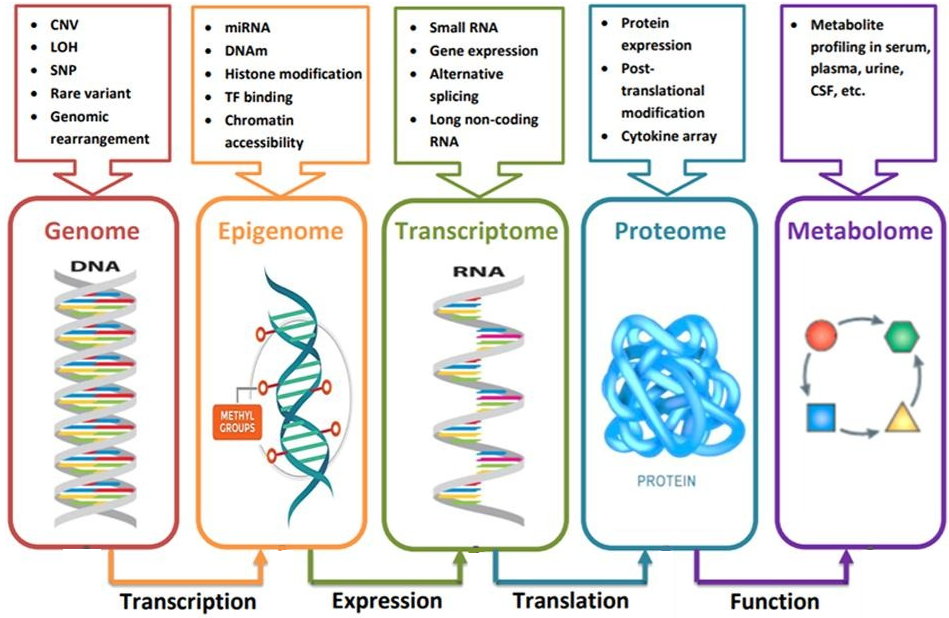
\includegraphics[width=1\textwidth]{figures/intro_omics.png}
 \caption[Méthodes de séquençages "omiques"]{\textbf{Schéma des différentes méthodes de séquençages "omiques"}. Les méthodes omiques donnent accès à une vue globale des mécanismes biologiques dans les tissus biologiques. (Modifié de \cite{momeni_survey_2020})}
 \label{fig:intro-omics}
\end{figure}
Les données de séquençage sont massives, le génome humain mesurant environ 3,1~milliards de paires de bases (bp), et le séquençage d'un génome unique avec une profondeur de 50X (nécessaire pour la détection de mutation génétique) représente un minimum de ~150 milliards de paires de bases lues et stockées, pour un individu. Ces données de séquence massives requièrent des outils spécifiques et un matériel informatique adapté à leur traitement. Outre l'aspect massif de ces données, la détection de mutations pathogènes est complexe. L'identification du gène responsable d'une maladie génétique reste un challenge lors du diagnostic, même avec les données de séquençage complètes.

\subsection{Ressources et initiatives en données biomédicales et maladies rares}\label{onto_ref}
Plusieurs ressources et initiatives ont été créées dans un effort de structuration des données biomédicales à travers la communauté scientifique. Une méthode de structuration de données très utilisée repose sur le concept d'ontologie. Les ontologies sont une représentation structurée et formelle d'entités et de leurs relations. Ces ontologies sont en quelque sorte un vocabulaire standard et universel développé de manière collaborative pour former un consensus sur les termes et leurs définitions.  Parmi les ontologies les plus utilisées dans le domaine biomédical on retrouve \textit{Human Phenotype Ontology}, (HPO, \cite{robinson_human_2008}, \cite{kohler_human_2021}), qui défini la liste des termes utilisés pour décrire les symptômes cliniques ou encore la \textit{Gene Ontology }(GO, \cite{the_gene_ontology_consortium_gene_2023}) qui défini la fonction des gènes, les processus biologies et les localisations cellulaires. À ce jour, le \textit{NCBI BioPortal} (\url{https://bioportal.bioontology.org/}) référence 1062 ontologies biomédicales développées et utilisées. Les ontologies utilisées dans le cadre de cette thèse sont présentées plus en détail dans le chapitre" Matériels et Méthodes" (\ref{mat_met_onto}). Ces ontologies sont très utiles pour structurer les données biomédicales grâce à des méthodes d'annotation qui vont reconnaitre les termes issus de ces ontologies dans les données non structurées telles que les textes libres. \\

En plus des ontologies, plusieurs bases de connaissances ont été développées, notamment dans la recherche sur les maladies rares. Parmi elles, on retrouve la base de données \textit{Online Mendelian Inheritance in Man (OMIM} \cite{amberger_omimorg_2015}) qui répertorie toutes les maladies héréditaires humaines connues, le gène associé et les phénotypes observés. Il y a également \textit{RD-Connect} (\cite{laurie_rd-connect_2022}), un projet européen permettant de connecter les bases de données existantes, les registres de patients et les biobanques en une plateforme centrale et disponible. Enfin, Orphanet (\cite{maiella_orphanet_2013}) est une initiative française qui développe à la fois une ontologie des maladies rares (\textit{ORDO}) mais qui est aussi un immense portail d'information destiné aux maladies rares qui répertorie des données sur les professionnels de santé, les centres experts, les études cliniques, de médicaments orphelins et de projets de recherches. L'ensemble de ces ressources représentent une base de connaissance importante qui peut être utile à la structuration et à l'exploitation automatique des données biomédicales. 

\subsection{Collecte et utilisation des données biomédicales au service du patient}
Le Royaume-Uni est un pays pionnier dans la collecte et la mise à disposition de façon massive de données biomédicales à travers le \gls{nhs}. Cela s'illustre par exemple par le projet "100 000 génomes" lancé en 2012 qui a pour but de séquencer 100 000 génomes de patients Anglais pour améliorer la recherche et le diagnostic de maladies rares, certains cancers et maladies infectieuses (\cite{nunn_public_2019}). En avril 2022 a été publié le rapport de 112 pages intitulé: "\textit{Better, broader, safer: using health data for research and analysis}" (\cite{ben_goldacre_better_2022}), écrit par le professeur Ben Goldacre missionné par le \gls{nhs}. Ce rapport met en évidence les challenges et la stratégie à adopter pour une collecte et un usage à grande échelle de données biomédicales de patients. Le projet OpenSAFELY (\href{https://www.opensafely.org/}{https://www.opensafely.org/}), fondé par Ben Goldacre, est un exemple concret d'utilisation de données biomédicales au service de la recherche et de la prise en charge de patients. Ce projet, créé en juin 2020 pour lutter contre la pandémie de COVID-19, met à disposition des chercheurs des outils et des données biomédicales massives de patients. À ce jour, ce projet a permis la publication de plus de 80 publications scientifiques de recherches réalisées à partir de ces données. Des initiatives similaires mettent en évidence l'utilité des \textit{Big Data} biomédicales comme catalyseur de découvertes scientifiques, tel que le projet "Big Data to Knowledge" fondé par le \textit{National Institutes of Health (NIH)} (\cite{toga_big_2015}). Cette collecte et utilisation des données biomédicales se généralise et d'autres initiatives sont à l'œuvre notamment aux Etats-Unis avec le projet TopMed (\url{https://topmed.nhlbi.nih.gov/}) par exemple.

Outre la phase de collecte, la difficulté dans l'exploitation des données biomédicales réside dans la disponibilité de techniques d'analyse adaptées (\cite{wang_big_2019, ismail_requirements_2020}). Les données biomédicales étant volumineuses, complexes et multimodales, leurs explorations manuelles ou \textit{via} des ontologies et techniques de statistiques classiques ne sont pas suffisantes. Une solution réside dans l'utilisation de l'intelligence artificielle, et plus spécifiquement de la branche nommée l'apprentissage automatique (\textit{machine-learning}, ML) pour construire des systèmes capables d'exploiter ces données. De nombreuses techniques d'analyse des \gls{dse} reposent aujourd'hui sur l'utilisation de modèles \gls{ia} (\cite{yang_large_2022, de_mello_semantic_2022, li_electronic_2022}).

\section{Apprentissage automatique pour le traitement des données biomédicales}
Le \gls{ml} est une branche de l'\gls{ia} qui regroupe un ensemble d'algorithmes capables d'accomplir une tâche en apprenant d'un jeu de données. Dans cette section, nous allons définir les concepts de base du \gls{ml} tels que le format des données, les tâches qui peuvent être accomplies, les méthodes d'apprentissage et les principaux algorithmes utilisés.

\subsection{Les formats et partitionnements des données}
Les données sont le point critique des techniques de \gls{ml}. Elles représentent l'ensemble des informations utilisées par un algorithme de \gls{ml} pour réaliser son apprentissage et réaliser des prédictions. Pour être utilisables par les algorithmes de \gls{ml}, les données doivent être structurées. Le tableau \ref{table:dataset_intro} présente un exemple de structure d'un jeu de données exploitable par un algorithme de \gls{ml}. Les données sont sous la forme de tableau où chaque ligne représente une observation (par exemple un patient) et chaque colonne représente un descripteur (nommé \textit{feature} en anglais, par exemple le rythme cardiaque, la présence d'une toux chez le patient, la présence d'antécédents de diabète dans la famille...). Enfin, la dernière colonne représente le label, que l'on souhaite prédire dans le cadre de l'entrainement de notre modèle.
\begin{table}[!ht]
\centering
\begin{tabular}{|c|c|c|c|c|} 
 \hline
 ID Patient & Rythme Cardiaque (bpm) & Toux & Diabète & Diagnostic \\
 \hline
 1 & 86 & non & non & Sain \\ 
 2 & 65 & ? & non & Sain \\ 
 3 & 59 & non & ? & Sain \\ 
 4 & 95 & oui & non & Malade \\ 
 5 & 101 & oui & oui & Malade\\ 
 \hline
\end{tabular}
\caption[Exemple de tableau de données fictives de patients]{\textbf{Exemple de tableau de données fictives de patients}}
\label{table:dataset_intro}
\end{table}
Cette contrainte sur la structure nécessaire du jeu de données pour les algorithmes de \gls{ml} met en évidence les limites de leurs utilisations pour l'analyse de données non structurées telles que le texte libre, les données d'imagerie. Il est nécessaire en amont de structurer ces données à travers des descripteurs pertinents pour les exploiter.

De plus, il est nécessaire de partitionner ce jeu de données sous forme de deux tableaux: les données d'apprentissage et les données de test. Les données d'apprentissage sont les données qui vont être utilisées par l'algorithme de \gls{ml} pour réaliser son entrainement, c'est-à-dire pour apprendre à réaliser la tâche définie (prédiction du label par exemple). Le jeu de test quant à lui contient des données qui n'ont jamais été présentées au modèle au cours de l'apprentissage. Le modèle entrainé va alors prédire le label du jeu de test et les prédictions réalisées sont comparées aux labels réels. Cela permet d'évaluer les performances d'un entrainement. Pour donner un ordre de grandeur, il est commun d'utiliser 80\% des données comme jeu d'entrainement et 20\% des données restantes comme jeu de test.

Pour finir, il existe un troisième partitionnement des données optionnel nommé jeu de validation. Le jeu de validation est réalisé en général en prenant 10\% des données d'entrainement. Ce jeu de validation permet d'évaluer le modèle au cours de l'entrainement et ajuster ses paramètres. Ceci permet de s'assurer que l'entrainement progresse correctement avant de tester les performances à la fin de l'entrainement sur le jeu de test.

\subsection{Les différentes tâches que le \textit{machine-learning} peut accomplir}
Les algorithmes de \gls{ml} peuvent accomplir de multiples tâches, dont quatre principales : (i) les algorithmes de classification (ii) de régression (iii) de \textit{clustering} et (iv) de réduction de dimensionnalité.

Les tâches de classification sont les plus communes. Il s'agit ici d'apprendre à prédire une classe ou un label pour un point de donnée. Par exemple, dans le cadre de données biomédicales, il peut s'agir de la prédiction d'un diagnostic parmi une liste de maladies. Cette classification peut-être binaire (2 classes uniquement, par exemple sain vs malade) ou multi-classe (plus de 2 classes, par exemple faire la différence entre 10 maladies potentielles). Enfin, cette classification peut aussi être multilabel, c'est-à-dire que l'on peut prédire plusieurs classes pour un point de donnée. Par exemple, si l’on construit un algorithme capable de prédire la fonction d'un gène, il est utile d'avoir un système de classification multilabel pour prédire les différentes fonctions dans lesquels un seul et même gène est impliqué. Parmi les algorithmes de \gls{ml} capables de faire de la classification, on retrouve de nombreux outils (décrit dans la section \ref{xai-sec}) tels que les méthodes bayésiennes, les méthodes à base d'arbres (arbre de décision, forêt aléatoire) ou encore les systèmes de classeurs.

Les tâches de régression ne cherchent pas à prédire une catégorie, mais une valeur numérique. Par exemple, on peut construire un modèle \gls{ml} capable de prédire le prix d'une maison ou encore la pression sanguine d'un patient, dans ces cas-là on cherche à prédire une valeur numérique continue. Les algorithmes à base d'arbres (arbre de décision, forêt aléatoire) sont aussi capables de réaliser des tâches de régression et on retrouve aussi d'autres algorithmes tels que la régression Lasso, Ridge et régression linéaire, qui est l'algorithme de base pour les tâches de régression.

Les tâches de \textit{clustering} cherchent à regrouper les points de données similaires en sous-groupes (c'est-à-dire en \textit{clusters}). Les techniques de \textit{clustering} sont utilisées dans le domaine biomédical pour analyser les données d'expression génétique par exemple. À partir de l'expression des gènes d'une cohorte de patients, il est possible d'utiliser des algorithmes de \textit{clustering} pour stratifier des sous-groupes de patients ayant un profil d'expression similaire (en cancérologie par exemple). Les algorithmes classiques de \textit{clustering} sont l'algorithme K-means (\cite{macqueen_methods_1967}), DBSCAN (\cite{ester_density-based_1996}) et le \textit{clustering} hiérarchique (\cite{cohen-addad_hierarchical_2017}).

Pour finir, les tâches de réduction de dimensionnalité consistent à réduire le nombre de variables aléatoires d'un jeu de données en obtenant un ensemble de variables principales. Typiquement, les données à haute dimensionnalité comme les données transcriptomiques (expression de plusieurs dizaines de milliers d'ARN) sont complexes à analyser et présentent des problèmes spécifiques à cette haute dimensionnalité, connus sous le nom de la malédiction de la dimension (\textit{curse of dimensionality}). Les techniques de réduction de dimensionnalité tendent à atténuer ce problème. Les algorithmes de réduction de dimensionnalité sont typiquement utilisés après une étape de \textit{clustering} pour observer graphiquement les \textit{clusters} obtenus en un graphique 2D. Pour reprendre l'exemple précédent, après une analyse transcriptomique, une étape de réduction de dimensionnalité permet de visualiser le principal axe de différenciation des échantillons. La réduction de dimensionnalité peut aussi être utilisée pour sélectionner les descripteurs les plus pertinents pour une tâche de classification. Les algorithmes de réduction de dimensionnalité communément utilisés sont la PCA (\cite{mackiewicz_principal_1993}), le t-SNE (\cite{maaten_visualizing_2008}) et UMAP (\cite{mcinnes_umap_2020}).

\subsection{Apprentissage supervisé, non supervisé et par renforcement}
Les différentes tâches présentées peuvent se regrouper sous trois méthodes d'apprentissages différentes: l'apprentissage supervisé, non supervisé et par renforcement.

Les tâches de classification et de régression sont possibles grâce à l'apprentissage supervisé. En apprentissage supervisé, le modèle est entrainé sur des données labellisées, c'est-à-dire des données pour lesquels on connait déjà le résultat attendu (diagnostic par exemple). Ainsi le modèle est entrainé à reproduire ces labels automatiquement.
Les tâches de \textit{clustering} et de réduction de dimensionnalité sont possibles grâce à l'apprentissage non supervisé. En apprentissage non supervisé, les labels des données ne sont pas connus par l'algorithme. L'objectif est donc de découvrir la structure cachée des données à partir des descripteurs. Ainsi le modèle essaie de déterminer des sous-groupes ou des regroupements de dimensions qu'il détermine comme pertinents, mais sans connaitre le résultat réel attendu.

Enfin, l'apprentissage par renforcement est moins connu et représente une méthode d'apprentissage où un agent (modèle) apprend à se comporter dans un environnement donné, recevant des pénalités et des récompenses en fonction de ses actions. Typiquement, un modèle apprenant à jouer à un jeu d'échecs représente une tâche d'apprentissage par renforcement. Dans un cadre biomédical, un système d'apprentissage par renforcement peut être utile par exemple pour un système d'examen médical intelligent qui va proposer des symptômes à vérifier chez le patient en fonction des observations déjà enregistrées. Ainsi, on a un environnement (les observations réalisées chez le patient) et des actions à réaliser par le modèle de \gls{ml} (proposer des symptômes ou examens à vérifier). Les algorithmes utilisés pour ce type d'apprentissage peuvent être des réseaux de neurones, les méthodes de \textit{Q-learning} ou encore les systèmes de classeurs.

La figure \ref{fig:ml-landscape} représente schématiquement la classification des tâches, des modes d'apprentissages et des différents cas d'applications et algorithmes associés.
\begin{figure}[!ht]
 \centering
 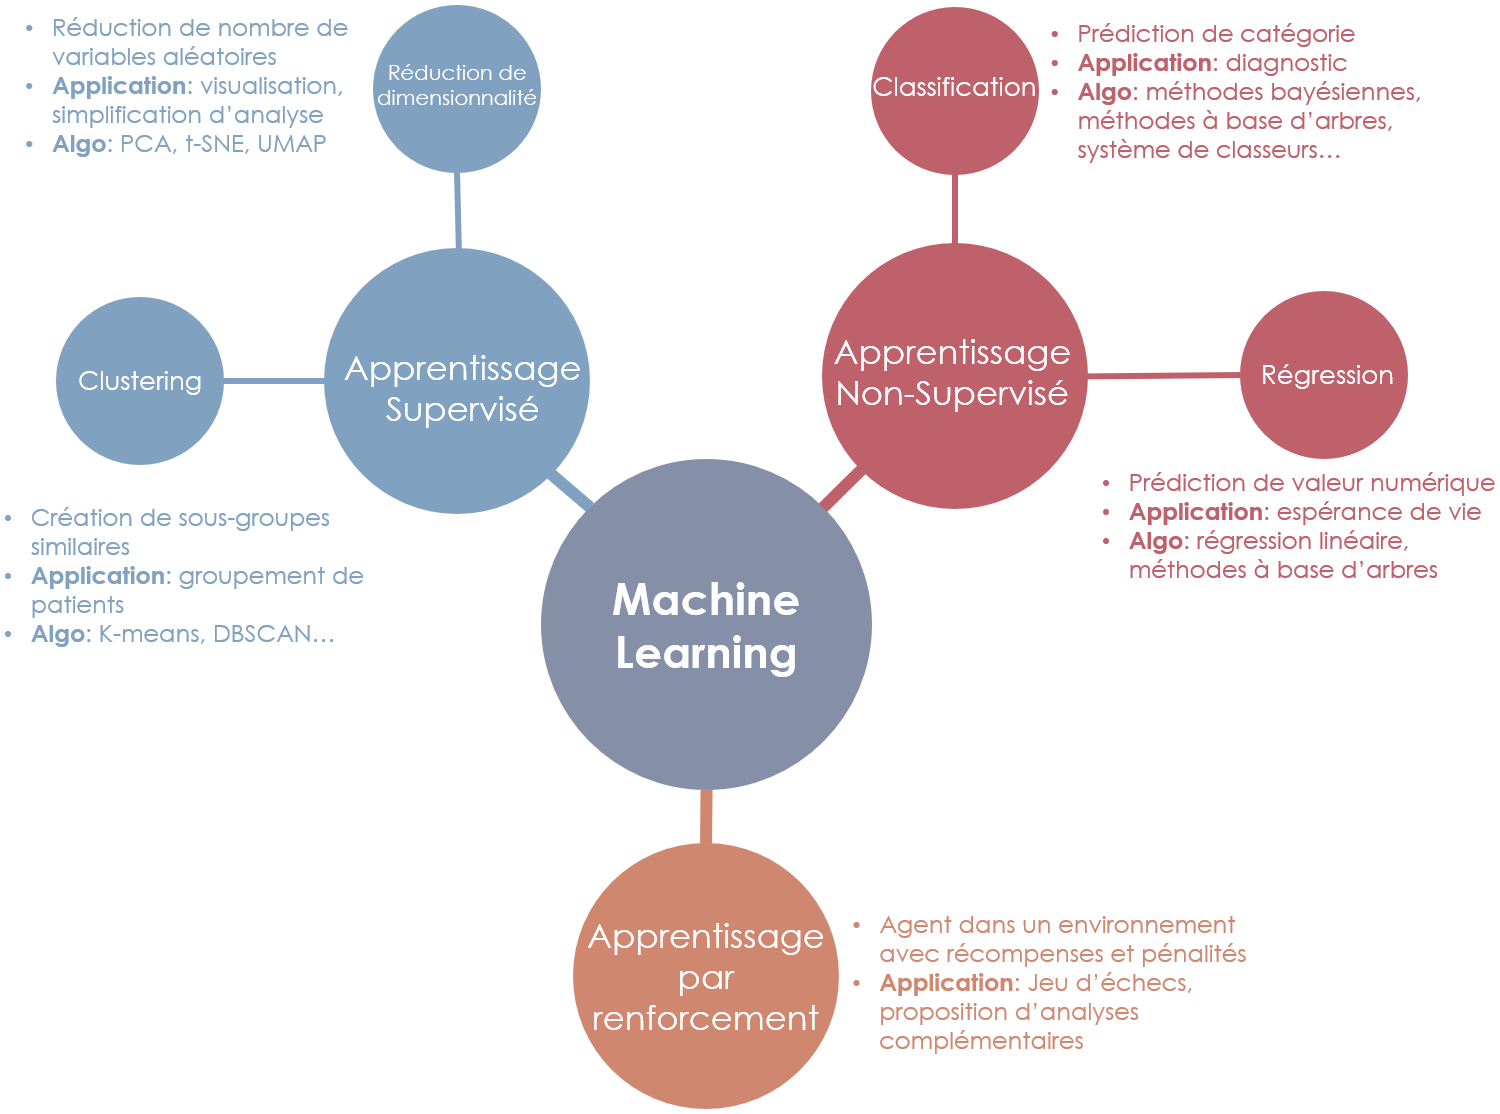
\includegraphics[width=1\textwidth]{figures/ml_landscape.png}
 \caption[Schéma des méthodes de machine-learning]{\textbf{Schéma de la classification des tâches, des modes d'apprentissage et des différents cas d'applications et algorithmes associés en \textit{machine-learning}}}
 \label{fig:ml-landscape}
\end{figure}

\subsection{Algorithmes de \textit{machine-learning} et explicabilité}\label{xai-sec}
Enfin, dans cette section de présentation des outils de \gls{ml}, nous allons présenter la notion d'explicabilité des algorithmes de \gls{ml} et son importance dans le domaine biomédicale. L'utilisation d'algorithmes explicables est cruciale dans le domaine de la santé, afin de pouvoir les utiliser en conditions réelles. Pour cela, les modèles de \gls{ml} entrainés et utilisés doivent être transparents, c'est-à-dire qu'on doit être capable de pouvoir comprendre et évaluer leurs prédictions. Cette transparence permet une confiance accrue dans le modèle à la fois par le patient et par le personnel médical, mais aussi d'éviter de potentielles erreurs. En effet lors d'un désaccord entre le personnel médical et une prédiction, il est alors possible dans le cadre d'un modèle transparent d'évaluer les raisons du désaccord pour prendre la meilleure décision possible pour le patient. Ainsi nous allons voir quelques exemples d'algorithmes de \gls{ml} couramment utilisés pour voir leur fonctionnement et leur niveau d'explicabilité.

\subsubsection{Le concept d'explicabilité}
D'après l'essai philosophique "\textit{Studies in the logic of explanation}" de Carl G. Hempel et Paul Oppenheim en 1948 (\cite{hempel_studies_1948}), le concept d'explication scientifique peut se résumer en une équation:
\[\sum C + \sum L = E\]
Dans cette équation, C représente l'ensemble des conditions antérieures et L représente l'ensemble des lois générales. La somme des conditions et des lois permet de produire E, l'évènement ou le phénomène observé. Les termes de gauche représentent ce qu’on nomme l’\textit{explanans} (l’expliquant) et le terme de droite est référé comme l’\textit{explanandum} (l’explicable). L’équation mathématique implique que l’on peut la lire dans les deux sens. C’est-à-dire qu’en connaissant E (le phénomène), nous pouvons déduire C et L (les conditions et lois) et nous réalisons donc une explication scientifique. À l’inverse, en connaissant C et L (les conditions et lois), nous pouvons déduire E (le phénomène) et nous faisons alors une prédiction. Optimalement, une explication est adéquate si l’\textit{explanans} permet de prédire totalement le phénomène observé.

Appliqué au \textit{machine-learning}, C représente alors les points de données et leurs descripteurs (conditions initiales), L représente notre modèle de \gls{ml} et ses règles internes, tandis que E représente la prédiction du modèle.

Les récentes recherches en \gls{ia} ont amené à l'émergence du domaine d'\gls{xai}. L'\gls{xai} cherche à concevoir des méthodes pour rendre les modèles d'\gls{ia} et de \gls{ml} plus transparents et explicables, ce qui est critique dans le cadre de l'application de ces modèles dans des domaines à haut risque, comme le domaine médical (\cite{arrieta_explainable_2019}). L'objectif est donc de concevoir des méthodes de \gls{ml} dont on est capable de comprendre et d'évaluer les prédictions de manière intelligible.

La figure (\ref{fig:xai-research}) présente le concept de compromis entre les performances des algorithmes et leur niveau d'explicabilité. De manière générale, plus un algorithme est performant d'un point de vue prédictif, moins il est explicable. Dès lors, le domaine de l'\gls{xai} va chercher : (i) à améliorer l'explicabilité des algorithmes performants et peu explicables ou (ii) à améliorer les performances des modèles les plus explicables.
\begin{figure}[!ht]
 \centering
 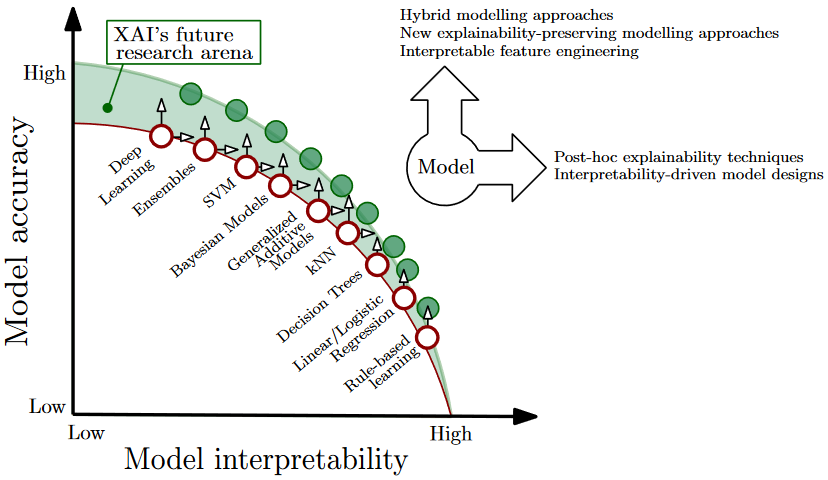
\includegraphics[width=1\textwidth]{figures/xai-research.png}
 \caption[Compromis entre interprétabilité et performances des algo de ML]{Compromis entre interprétabilité du modèle et performance d'algorithmes de ML. Représentation de la zone d'amélioration où réside le potentiel des techniques et outils de l'IA explicable (xAI) (Source: \cite{arrieta_explainable_2019})}
 \label{fig:xai-research}
\end{figure}

Au regard de l'explicabilité d'un modèle en \gls{ml}, il y a deux catégories d'algorithmes: (i) les algorithmes transparents par design, c'est-à-dire directement explicables et (ii) les algorithmes sous forme de boites noires, dont l'explicabilité n'est accessible que grâce à des méthodes \textit{post-hoc}. Dans les prochaines sous-sections, nous allons présenter le fonctionnement des algorithmes les plus utilisés de façon non exhaustif pour chaque catégorie. Nous allons ainsi voir les méthodes bayésiennes, les arbres de décisions et les systèmes de classeurs comme méthodes transparentes. Puis les méthodes de forêts aléatoires et de \textit{boosting} seront présentées comme méthodes à explicabilité \textit{post-hoc}.

\subsubsection{Méthodes bayésiennes}
Les méthodes bayésiennes naïves reposent sur le théorème de Bayes sur les probabilités conditionnelles avec une hypothèse d'indépendance forte (c'est-à-dire naïve) entre les descripteurs. Pour chaque descripteur, la probabilité d'une classe est calculée en fonction de la valeur du descripteur. Grâce à cette caractéristique probabiliste, le modèle est capable de fournir une prédiction et une mesure de l'incertitude associée. Les méthodes bayésiennes sont transparentes et donc explicables, car il est possible de décomposer la contribution de chaque descripteur lors d'une prédiction.

\subsubsection{Méthodes à base d'arbres}
Les arbres de décision sont des modèles classiques en \gls{ml}. Cette méthode cherche à produire un arbre (un graphe dirigé acyclique) où chaque nœud s'apparente à une série de questions posées sur les descripteurs des données. En fonction de la valeur de ces descripteurs, l'arbre progresse vers un sous-nœud jusqu'à la prédiction, le nœud feuille final. Cette méthode est intrinsèquement explicable, car il est facile de dessiner l'arbre et de retracer le processus de prédiction pour un point de données en suivant les nœuds comme une série de règles logiques. Par exemple, la figure \ref{fig:decision-tree} présente un exemple d'arbre de décision très simple avec trois nœuds (3 questions pour 3 descripteurs) et deux classes possibles comme prédiction (nœud feuille final rond).
\begin{figure}[!ht]
 \centering
 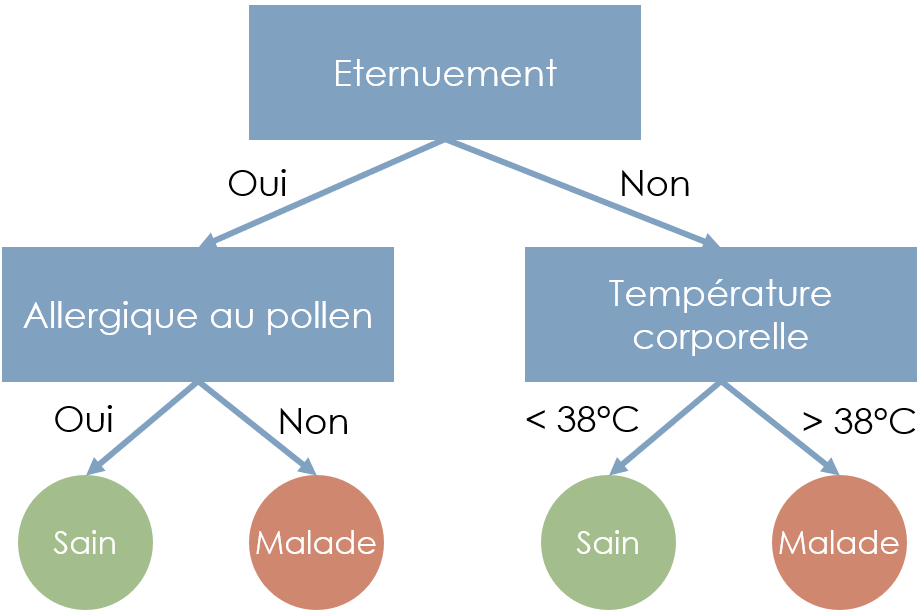
\includegraphics[width=0.6\textwidth]{figures/decision_tree.png}
 \caption[Exemple d'arbre de décision]{Exemple d'arbre de décision à 3 questions (3 nœuds pour 3 descripteurs) et 2 classes.}
 \label{fig:decision-tree}
\end{figure}

Une évolution des arbres de décision pour les rendre plus complexes et performants est nommée la méthode de la forêt aléatoire qui est une méthode ensembliste des arbres de décision. La figure \ref{fig:random-forest} présente le fonctionnement de la forêt aléatoire. Cela consiste à construire plusieurs arbres de décision sur des sous-ensembles des données, puis de combiner les prédictions de ces arbres. Chaque arbre de décision ainsi généré va établir une prédiction et la prédiction finale correspondra à la majorité des votes de chaque arbre. Les méthodes de \textit{boosting} (XGBoost (\cite{chen_xgboost_2016}), LGBoost (\cite{ke_lightgbm_2017}), CatBoost (\cite{prokhorenkova_catboost_2019})) sont similaires aux forêts aléatoires à la différence que chaque arbre n'est pas construit indépendamment, mais il cherche à corriger les erreurs du précédent, de manière séquentielle.
\begin{figure}[!ht]
 \centering
 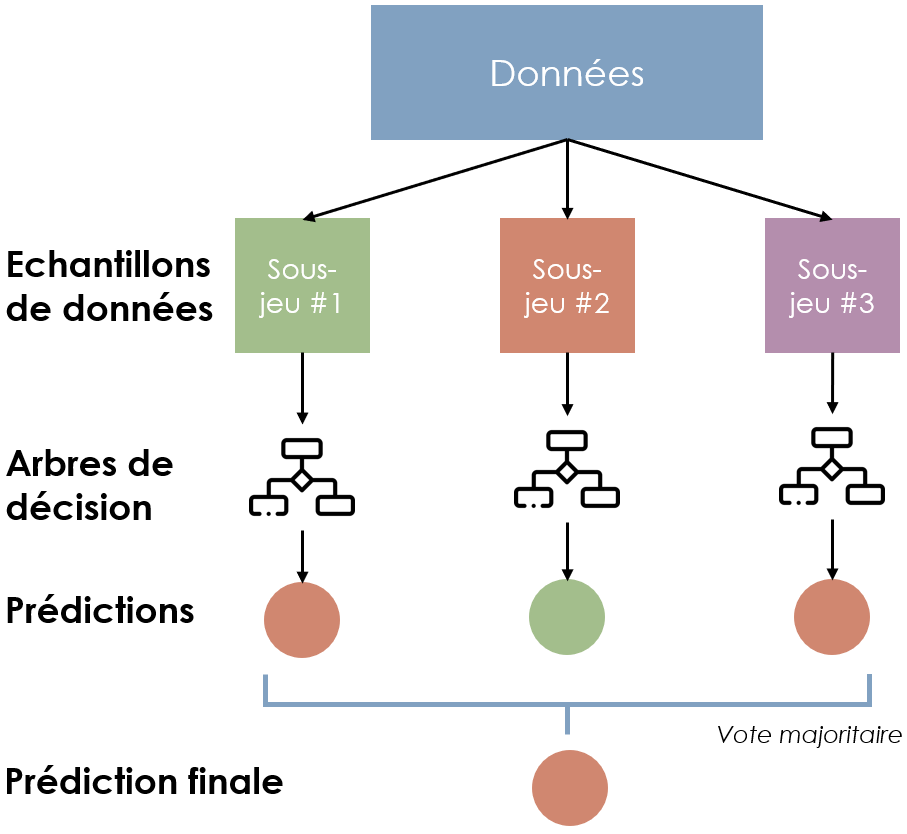
\includegraphics[width=0.7\textwidth]{figures/random_forest.png}
 \caption[Fonctionnement de l'algorithme de forêt aléatoire]{Fonctionnement de l'algorithme de forêt aléatoire}
 \label{fig:random-forest}
\end{figure}
Les forêts aléatoires sont très utilisées en \gls{ml} et spécifiquement en biologie. En exemple d'application dans le domaine biomédicale, l'outil MISTIC (\textit{MISsense deleTeriousness predICtor}, \cite{chennen_mistic_2020}) développé dans notre équipe utilise des méthodes de forêts aléatoires pour calculer la pathogénicité des variants génétiques. Cependant, la forêt aléatoire et les méthodes de \textit{boosting} perdent en explicabilité. En effet, en raison du grand nombre d'arbres de décision générés, il n'est plus possible de suivre aisément le processus de prédiction suivant une suite de règles logiques pour un point de donnée. Il faut alors utiliser des méthodes d'explicabilité \textit{post-hoc} qui consistent à calculer l'importance numérique de chaque descripteur pour une prédiction donnée.

\subsubsection{Systèmes de classeurs (LCS)}
Les \gls{lcs} sont des algorithmes de \gls{ml} parmi les plus transparents et explicables (\textit{"rules-based learning"} figure \ref{fig:xai-research}, \cite{arrieta_explainable_2019}). Ces systèmes fonctionnent sur le principe d'un ensemble de règles (nommées "classeurs"), qui associent des conditions à une action (prédiction). Le tableau \ref{table:lcs-rules} présente un exemple de trois règles fictives issues de l'entrainement d'un \gls{lcs}. Une règle (ou un classeur) se présente sous la forme "SI [condition] ALORS [prédiction]". Chaque règle est associée à un poids, ce qui permet de définir une importance plus ou moins forte. Leur fonctionnement est donc similaire aux arbres de décision, mais donc les règles sont évaluées sans ordre imposé.
\begin{table}[!ht]
\centering
\begin{tabular}{|l|l|c|} 
 \hline
 Conditions & Prédiction & Poids \\
 \hline
 SI éternuement ET allergique au pollen & ALORS sain & 7 \\ 
 SI temp. corporelle > 38°C & ALORS malade & 12 \\ 
 SI éternuement ET temp. corporelle = 37°C & ALORS sain & 3 \\ 

 \hline
\end{tabular}
\caption{Exemple de règles fictives issues de l'entrainement d'un algorithme de LCS}
\label{table:lcs-rules}
\end{table}

L'apprentissage des systèmes de classeurs se réalise par des mécanismes d'évolution. Chaque règle va être initialement générée de façon aléatoire (ou guidée, \cite{urbanowicz_relief-based_2018}) puis modifiée (mutée) aléatoirement au fur et à mesure des cycles d'entrainement (générations). À chaque cycle, les règles les moins performantes lors de l'évaluation sur le jeu d'entrainement sont éliminées du jeu de règles. Ainsi au bout d'un certain nombre de cycles (générations), les règles générées qui ont survécu au processus de sélection sont performantes dans leurs taches de classification.

Les \gls{lcs} sont extrêmement explicables, car leur apprentissage génère une liste de règles parfaitement intelligible pour l'Homme, ainsi il est facile de reproduire le processus de prédiction des points de données manuellement (\cite{arrieta_explainable_2019}). Aussi, pour chaque prédiction, il est possible de savoir exactement quelles règles ont été déclenchées et ont mené à cette prédiction. Cependant, ces systèmes restent sous-performants et leurs méthodes d'apprentissage par évolution posent des difficultés de mise à l'échelle et nécessitent un grand nombre de données pour être efficaces (\cite{urbanowicz_exstracs_2015}).

\subsection{Limites du \textit{machine-learning} appliqué aux données biomédicales}
Bien que les techniques de \gls{ml} se révèlent utiles pour traiter, analyser et prédire de grands ensembles de données, ces techniques font face à de grandes difficultés dans le cadre des données biomédicales (\cite{martinez-garcia_data_2022}). Les données biomédicales étant massives, mais surtout non structurées et multimodales, il est difficile de réaliser le travail d'annotation nécessaire à leurs structurations pour l'utilisation d'algorithme de \gls{ml}. Car l'annotation manuelle des données est un travail couteux en temps et en argent, d'autant plus dans le domaine médical ou l'annotateur doit être un expert du domaine. Ainsi il est nécessaire de développer des méthodes d'\gls{ia} capables d'apprendre et d'exploiter les données brutes non structurées sous toutes les formes (textes, images, séquences).

Dans ce contexte, les réseaux de neurones profonds présentent une opportunité pour le traitement des données biomédicales non structurées. En effet, les réseaux de neurones sont parmi les modèles les plus performants et sont capables de traiter aisément des données non structurées en extrayant eux-mêmes les descripteurs pertinents à partir de la structure des données. Cependant, ce sont aussi de complètes boites noires et non explicables. Une stratégie intéressante pour l'utilisation des réseaux de neurones profonds tout en gardant une explicabilité satisfaisante est de les coupler aux méthodes de \gls{ml} classiques. Il est possible d'utiliser ces réseaux de neurones sous forme de boites noires pour extraire des descripteurs pertinents à partir de données non structurées (par exemple, quantifier un marqueur pathologique sur une image). Puis dans un second temps, d'utiliser des méthodes de \gls{ml} classiques et explicables pour, à partir de ces descripteurs extraits, réaliser la tâche de classification et de diagnostic.

Dans le prochain chapitre, nous verrons comment les réseaux de neurones profonds fonctionnent et peuvent être utilisés pour traiter et extraire de l'information des données biomédicales non structurées là où les techniques de \gls{ml} classique échouent.
\chapter*{Chapitre 2: Réseaux de neurones profonds et exploitation de données complexes}
% ...
Placeholder
\chapter{L’exemple des myopathies congénitales et la difficulté du diagnostic}
\section{Le muscle, un organe avec une structure cellulaire particulière}
\subsection{Strucutre}
\subsection{Type de Muscle}
\section{Les myopathies congénitales}
\subsection{Description générale}
\subsection{Prévalence}
\subsection{Classification}
\subsection{Diagnostic}
\section{Données générées pour le diagnostic des myopathies congénitales}
\part{MATÉRIELS ET MÉTHODES}
\chapter{Outils informatiques et données utilisées}

Dans cette thèse nous avons développé des méthodes basées sur les \gls{ia}s pour exploiter les données multimodales de patients. Pour cela, nous avons utilisé un vaste panel de ressources biologiques, d'outils informatiques et de méthodes \gls{ia}. Dans ce chapitre, nous allons décrire l'ensemble des outils et ressources utilisés pour construire nos méthodes d'analyse.

\section{Données biomédicales de myopathies congénitales}
Nous avons développé des méthodes \gls{ia} pour analyser des jeux de données multimodales de myopathies congénitales. Pour développer ces méthodes, nous nous sommes basés sur des données d'imagerie et des comptes rendus de biopsie. La source de ces données est présentée ci-dessous.

\subsection{Comptes rendus de biopsie de l'institut de myologie de Paris}
La première source de données provient de l'institut de myologie de Paris. Grâce à une collaboration avec l'équipe du laboratoire d’histopathologie d'abord dirigé par Norma B. Romero puis Teresinha Evangelista, nous avons pu récupérer et utiliser 192 comptes rendus de biopsie musculaire de patients atteints de myopathies (congénitales, dystrophies ou autre), dont 138 spécifiquement atteint par des myopathies congénitales identifiées. Ces rapports sous format papier ont été scannés puis anonymisés d'abord avec un outil d'anonymisation que nous avons développé (présenté dans le chapitre 7), puis vérifiés à la main. La figure \ref{fig:compte-rendu-exemple} présente la structure d'un compte rendu anonymisé de biopsie typique présent dans le jeu de données. Il y a deux types de comptes rendus, ceux qui concernent les observations en microscopie photonique et ceux qui concernent les observations en microscopie électronique. Cependant, cette structure peut varier en fonction de l'année de production du compte rendu, certains sont totalement déstructurés.

\begin{figure}[!ht]
 \centering
 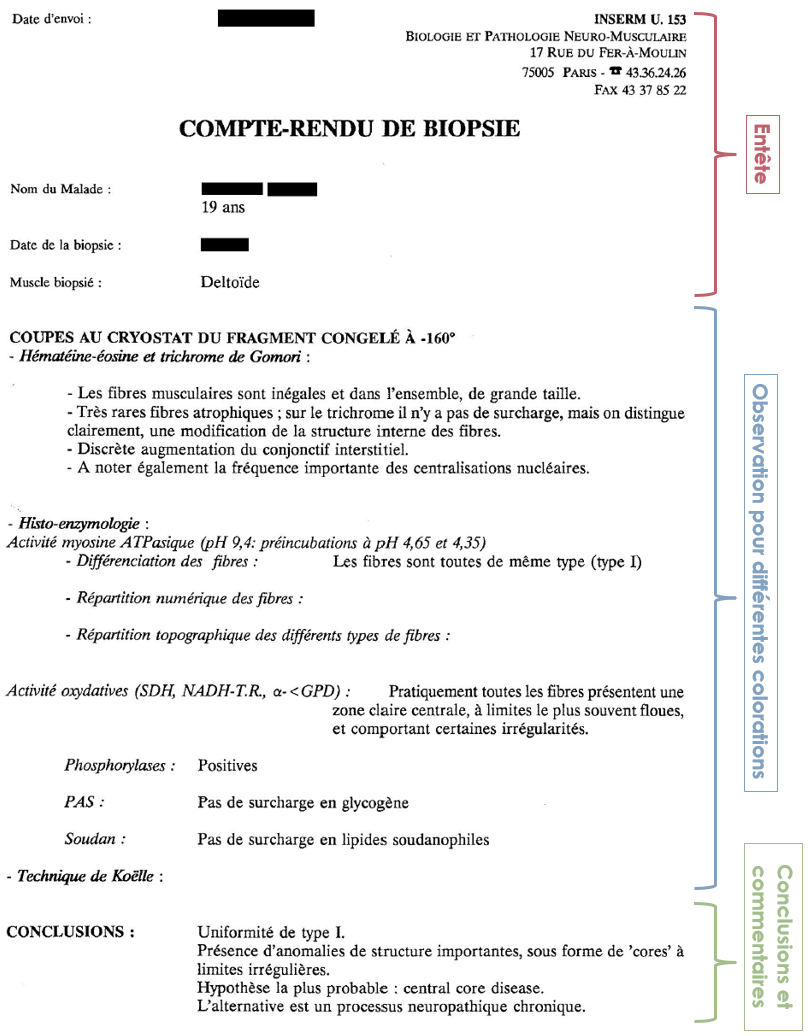
\includegraphics[width=0.9\textwidth]{figures/compte_rendu_exemple.png}
 \caption[Exemple de compte rendu de biopsie]{Exemple de compte rendu de biopsie en microscopie photonique anonymisé de l'institut de myologie de Paris}
 \label{fig:compte-rendu-exemple}
\end{figure}

\subsection{Images de biopsie musculaire de souris}
Une seconde source de données provient d'une collaboration avec l'\gls{igbmc}, plus spécifiquement avec l'équipe Physiopathologie des maladies neuromusculaires dirigée par Jocelyn Laporte. Cette équipe travaille sur les myopathies congénitales et utilise plusieurs souris modèles de myopathies congénitales. Ainsi en travaillant avec les membres de l'équipe réalisant des biopsies musculaires sur ces modèles, nous avons développé des méthodes d'analyse pour des biopsies musculaires de souris aux colorations \gls{he}, \gls{sdh}, ATPase et à fluorescence.

\section{Ontologies biologiques}
En biologie, les ontologies sont des vocabulaires standards pour faciliter l'intégration des données et leur analyse. Dans cette thèse, pour standardiser les données issues des comptes rendus, notamment dans le cadre du développement de l'outil \gls{impatient} et l'analyse de sa base de données, nous avons utilisé diverses ontologies préexistantes que nous allons décrire ici.

\subsection{Ontologie des phénotypes : HPO}
L'ontologie \gls{hpo}, développée en 2008 par Peter N Robinson et Sebastian Köhler au \textit{Charité University Hospital} à Berlin (\cite{robinson_human_2008}, \cite{kohler_human_2021}), rassemble l'ensemble des phénotypes médicaux observables chez l'Homme. Organisée sous forme d'arbre, elle contient plus de 13 000 termes organisés selon un niveau croissant de précision (par exemple le terme "anomalie de l'œil" est un parent du terme "anomalie de la pupille"). Chaque terme est associé à un identifiant unique sous la forme HPO:XXXXX et possède un certain nombre d’annotations comme des maladies associées, des gènes associés, des synonymes, des publications associées. L'ensemble de ces informations est disponible en ligne sur le portail  \href{https://hpo.jax.org/}{https://hpo.jax.org/} qui permet aussi de télécharger l'ontologie dans les formats standards (JSON, OBO, OWL). Cette ontologie est utilisée dans \gls{impatient} pour normaliser les observations cliniques des patients.

\subsection{Ontologie de maladies : ORDO par Orphanet}
L'\gls{ordo} est née d'une collaboration entre Orphanet (\href{https://www.orpha.net/}{https://www.orpha.net/}, \cite{maiella_orphanet_2013}), et l'Institut Européen de Bioinformatique (EBI). Orphanet est une ressource informatique ayant pour but de répertorier l'ensemble des informations concernant les maladies rares et les médicaments orphelins. L'ontologie ORDO répertorie plus de 7 000 maladies rares connues. Chaque maladie rare est répertoriée sous un identifiant unique de la forme ORPHA:XXXXXX, par exemple la maladie "Myopathie congénitale sévère à némaline" correspond à l'identifiant ORPHA:171430. De plus, chaque maladie est associée à des annotations telles que leur prévalence, des synonymes, un mode d'hérédité, un âge d'apparition, un pronostic, les gènes causant la maladie et autre. Pour finir, chaque maladie est aussi liée à des symptômes cliniques grâce à un lien direct vers des identifiants de l'ontologie \gls{hpo}. Dans le cadre de notre outil \gls{impatient} nous avons utilisé cette ontologie pour normaliser le diagnostic final des patients.

\subsection{Nomenclature génétique : HGNC et HGVS}
L'ontologie HUGO (\href{https://www.genenames.org/}{https://www.genenames.org/}, acronyme de Human Genome Organisation, est gérée par le Comité de Nomenclature des Gènes de HUGO (HGNC) à l'Institut Européen de Bioinformatique. Ce comité est responsable de l'attribution de noms uniques pour les gènes humains, que ce soit des gènes codants pour des protéines, gènes non codants ou pseudogènes. Au total, plus de 43 000 noms de gènes uniques sont référencés et annotés avec des références vers des bases de données externes (banque de séquences, orthologies, mutations, structures, Orphanet…). Concernant les variations génétiques (mutations), la nomenclature établie par la \gls{hgvs} (\href{https://www.hgvs.org/}{https://www.hgvs.org/}) fait autorité. Cette nomenclature spécifie la façon de représenter textuellement un variant génétique. Par exemple selon cette nomenclature la notation "LRG\_199p1:p.Trp24Cys" indique une mutation faux-sens dans la protéine LRG\_199 où l'acide aminé n° 24 est substitué d'un tryptophane à une cystéine. L'ontologie HUGO et la nomenclature HGVS sont toutes deux intégrées dans \gls{impatient} pour normaliser le diagnostic génétique des patients (gène muté et localisation de la mutation responsable de la maladie).

\section{Développement de modèles de ML traditionnels et xAI}
Dans le cadre de l'analyse de la base de données de \gls{impatient} et des résultats d'\textit{embedding} de \gls{nlmyo} nous avons utilisé des algorithmes de \gls{ml} traditionnels pour créer des modèles prédictifs. Dans cette section, nous présentons les principaux outils utilisés en ce qui concerne les algorithmes utilisés et l'analyse de leurs performances.

\subsection{\textit{Scikit-Learn} : une boite à outils pour l'apprentissage automatique}
\textit{Scikit-Learn} (\cite{pedregosa_scikit-learn_2011}, \href{https://scikit-learn.org/}{https://scikit-learn.org/}) est une bibliothèque de code python mettant à disposition un grand nombre d'outils et permettant de préparer les données, d'entrainer des modèles de \textit{\gls{ml}} et d'évaluer ses performances. \textit{Scikit-learn} inclut des algorithmes de classification, de régression, de clustering, de réduction de dimensionnalité, d'optimisation et de sélection de modèles. Scikit-learn a été utilisé dans cette thèse pour : (i) partitionner et normaliser les données, (ii) entrainer des modèles de classification de différentes familles d'algorithmes, (iii) optimiser et évaluer les performances des modèles.

\subsection{Validation croisée et évaluation des performances}
La validation croisée (\textit{cross-validation }en anglais) est une technique d'évaluation de modèles prédictifs permettant d'avoir une estimation plus robuste et précise des métriques de performance. Cette méthode est particulièrement utile pour les jeux de données de petite taille. La figure \ref{fig:cross-val} présente schématiquement son fonctionnement. Le jeu de données initial est séparé en N sous-ensembles (nommés \textit{folds}, ici au nombre de 5). Ensuite le modèle est entrainé sur l'ensemble des sous-ensembles à l'exception d’un, qui est utilisé comme jeu de test des performances. Ce processus est répété autant de fois qu'il y a de \textit{folds} afin que chaque \textit{fold} ait été utilisé exactement une fois comme jeu de test. Ainsi pour 5 \textit{folds}, cinq modèles sont entrainés et évalués. On peut alors calculer une performance moyenne du modèle entrainé sur l'ensemble des données, en calculant les performances moyennes des cinq modèles. Plus le nombre de \textit{folds} est important, plus cette moyenne est précise, mais c'est plus coûteux en temps et ressources de calcul, car il faut entrainer plus de modèles.
\begin{figure}[!ht]
 \centering
 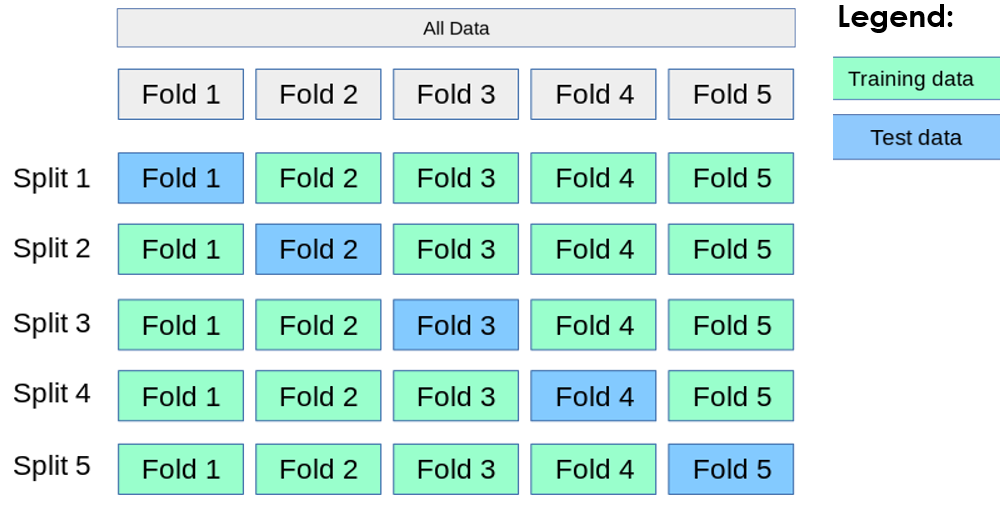
\includegraphics[width=0.9\textwidth]{figures/cross-val.png}
 \caption[Schéma validation-croisée]{Schéma du principe de la validation croisée (modifié de la documentation de \textit{Scikit-Learn})}
 \label{fig:cross-val}
\end{figure}
\subsection{Recherche d'hyperparamètres}
La recherche d'hyperparamètres est une étape importante dans le développement de modèles prédictifs pour améliorer les performances des modèles. Les hyperparamètres sont des paramètres propres à chaque algorithme, qui sont spécifiés en amont de l'entrainement et qui ne varient pas lors de l'entrainement, mais qui influent directement sur les performances du modèle. Par exemple, dans le cadre de l'entrainement d'un arbre de décision, un exemple d'hyperparamètre peut être la profondeur maximale de l'arbre ou encore la méthode de calcul de qualité d'un nœud (par exemple méthode de gini ou entropie).
\begin{figure}[!ht]
 \centering
 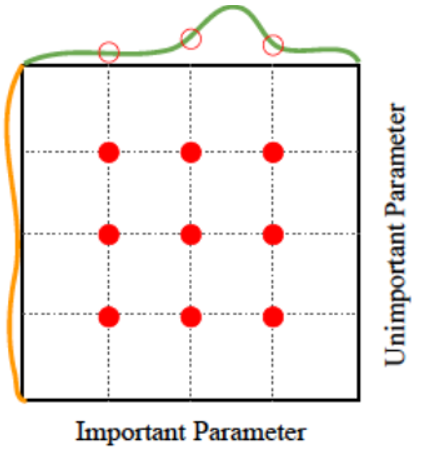
\includegraphics[width=0.3\textwidth]{figures/parameters_grid.png}
 \caption[Schéma rechercher hyper-paramètres]{Schéma du principe de recherche d'hyperparamètres par grille pour 2 paramètres. Un point rouge représente un modèle entrainé. }
 \label{fig:params_grid}
\end{figure}
La recherche d'hyperparamètres revient à trouver une combinaison de paramètres optimale qui maximise les performances du modèle après entrainement. La méthode la plus classique pour cela est l'optimisation par grille. À partir d'un ensemble de valeurs possibles pour chaque paramètre, on va entrainer et tester les performances du modèle pour chaque combinaison de valeurs et sélectionner la combinaison de valeurs la plus performante. La figure \ref{fig:params_grid}  présente un exemple théorique d'optimisation par grille pour deux paramètres. Pour chacun des paramètres, 3 valeurs sont possibles, c'est donc un total de 9 modèles qui sont entrainés et testés. On peut alors mesurer l'impact de chaque paramètre sur les performances finales du modèle pour trouver le paramètre le plus important et sa valeur optimale.
D'autres méthodes moins naïves et moins coûteuses que la grille existent pour la recherche d'hyperparamètres telle que l'approche bayésienne utilisée par la bibliothèque de code \textit{Optuna} (\cite{akiba_optuna_2019},\href{https://optuna.org/}{https://optuna.org/}) qui permet de trouver une combinaison optimale plus rapidement.

\subsection{Algorithme de système de classeurs : ExSTraCS 2.0}
Les systèmes de classeurs sont une famille d'algorithmes de \gls{ml} considérés comme explicables. Dans cette thèse, nous avons utilisé le \gls{lcs} nommé \textit{ExSTraCS 2.0} (\cite{urbanowicz_exstracs_2015}), spécifiquement développé pour les tâches de classification à partir de données complexes, hétérogènes et de haute dimensionnalité. Cet algorithme a été utilisé pour tenter de prédire le diagnostic de sous-type de myopathies congénitales des patients à partir des annotations réalisées dans \gls{impatient}. L'implémentation en Python de cet algorithme de \gls{lcs} nommée \textit{scikit-ExSTraCS} (\href{https://github.com/UrbsLab/scikit-ExSTraCS}{https://github.com/UrbsLab/scikit-ExSTraCS}) nous a permis d'entrainer un modèle basé sur cette méthode et de comparer ses performances aux autres algorithmes implémentés dans \textit{scikit}, via le pipeline d'entrainement et de comparaison de modèles nommé \textit{Streamline}.

\subsection{Streamline: un pipeline d'entrainement et de comparaison de modèles ML}
Dans le cadre de l'analyse de la base de données d'\gls{impatient}, nous avons voulu entrainer le modèle de classification (prédiction de diagnostic) le plus performant possible et de manière reproductible. Pour cela nous avons utilisé le pipeline d'entrainement et de comparaison de modèles de \gls{ml} nommé \textit{Streamline} (\cite{urbanowicz_streamline_2023}). La figure \ref{fig:streamline} présente son fonctionnement. Il y a 4 étapes principales. L'étape 1 (modules 1 et 2) consiste en la lecture, exploration statistique et préparation des données. L'étape 2 (modules 3 et 4) consiste au calcul de l'importance de chaque annotation (comprendre ici : \textit{feature}) et en la sélection des annotations les plus pertinentes pour la classification. L'étape 3 (module 5) consiste à l'optimisation et l'entrainement de 16 algorithmes de \gls{ml} variés et l'évaluation des performances des modèles issus de cet entrainement. Finalement, l'étape 4 (modules 6, 7, 8  et 9) correspond à la phase de posttraitement, où seront générés les figures de comparaison des performances des modèles et le nettoyage des fichiers. STREAMLINE n'est pour l'instant disponible que pour faire de la classification binaire. Nous nous intéressons à un problème de classification multi-classe (prédiction de diagnostic), donc nous avons modifié le pipeline pour le rendre compatible avec nos données. Le code du pipeline modifié est accessible à l'adresse \href{https://github.com/lambda-science/STREAMLINE}{https://github.com/lambda-science/STREAMLINE}.
\begin{figure}[!ht]
 \centering
 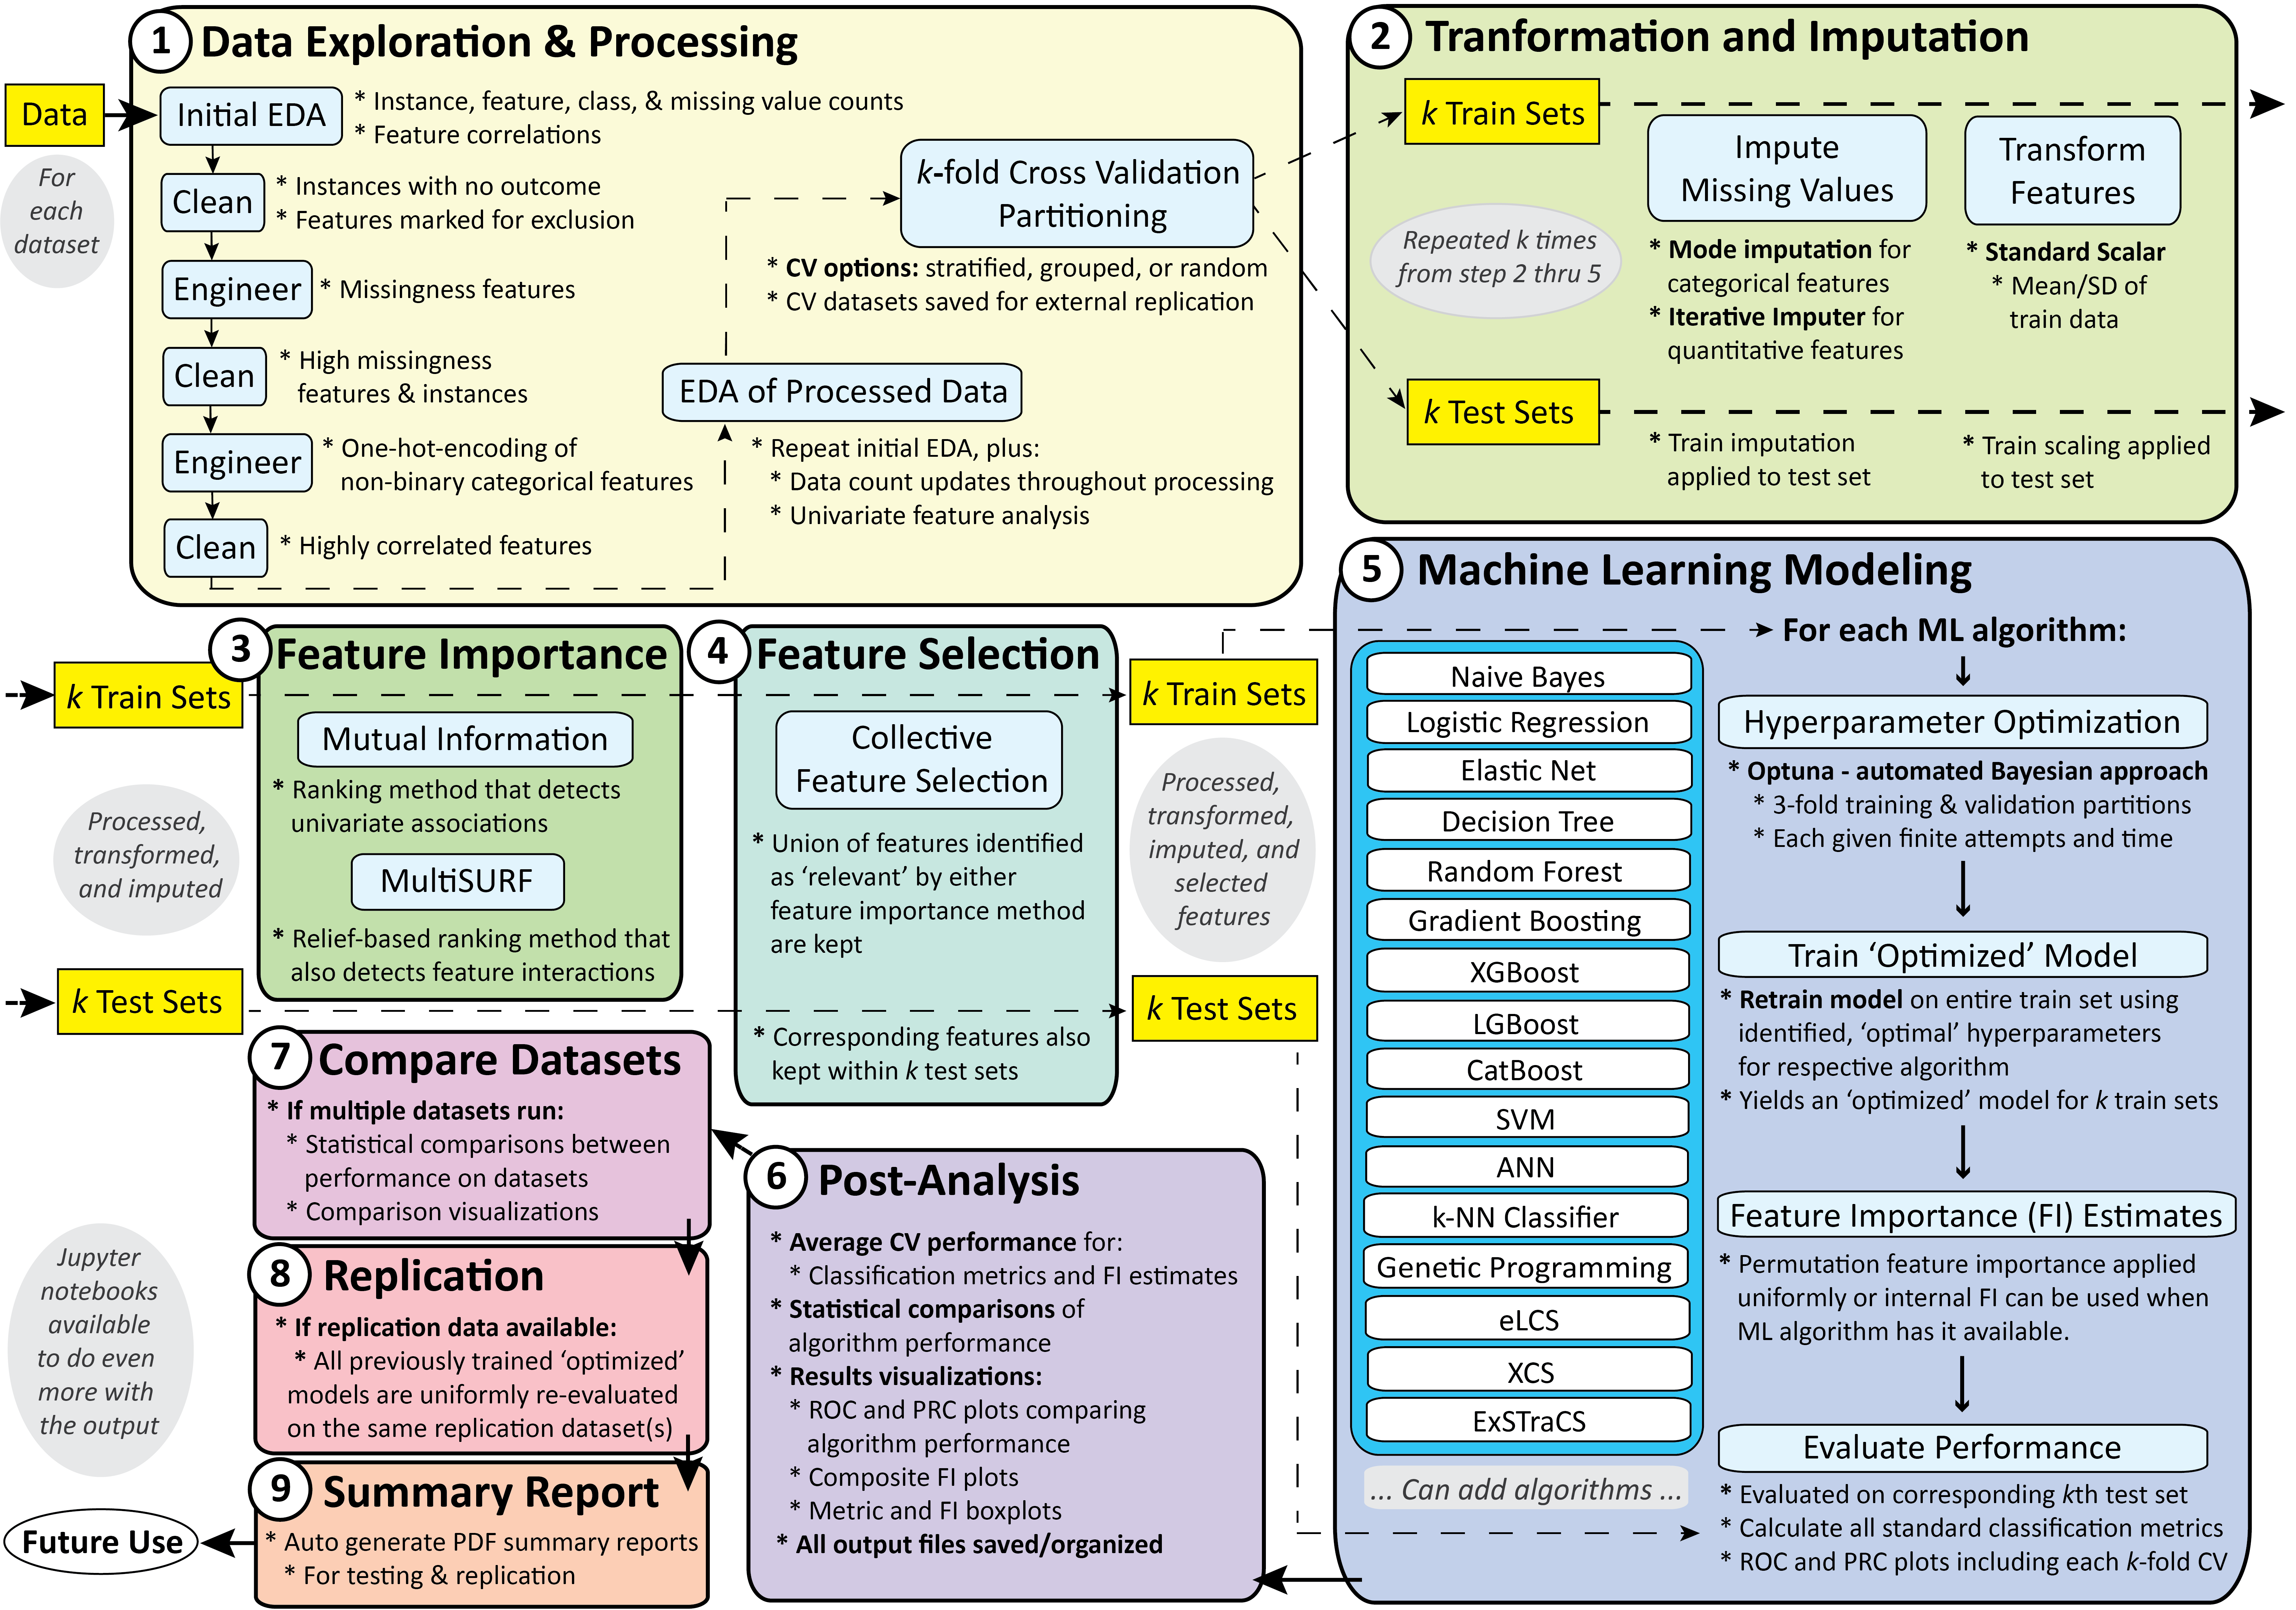
\includegraphics[width=1\textwidth]{figures/STREAMLINE_paper_lightcolor.png}
 \caption[Pipeline STREAMLINE]{Schéma du pipeline STREAMLINE}
 \label{fig:streamline}
\end{figure}
\subsection{Métriques de performance}
Pour évaluer les performances de nos modèles, nous avons utilisé plusieurs métriques. Dans le cadre d'une classification multi-classe et déséquilibrée, la mesure de l'exactitude de classification (\textit{accuracy}) n'est pas suffisante pour obtenir une bonne représentation des performances des modèles. Ainsi nous mesurons aussi l'exactitude équilibrée (\textit{balanced accuracy}), le score F1, score F1 macro, la spécificité et le coefficient de corrélation de Matthew. L'ensemble de ces métriques de performance, décrites dans la section suivante, sont calculées à partir de la matrice de confusion.

\subsubsection{Matrice de confusion}
La matrice de confusion est une matrice en deux dimensions qui compare  les prédictions d'un modèle par rapport aux labels réels des données. Par exemple pour une classification en 3 classes, une matrice de confusion de taille (3x3) est produite. La diagonale (haut gauche vers bas droit) représente l'ensemble des prédictions correctes (vrais positifs et vrais négatifs) c'est-à-dire les points pour lesquels la prédiction est en accord avec le label réel. Les autres cases représentent l'ensemble des prédictions incorrectes (faux positifs ou faux négatifs). La figure \ref{fig:confusion-example}  représente un exemple de matrice de confusion pour une classification binaire en 2 classes.
\begin{figure}[!ht]
 \centering
 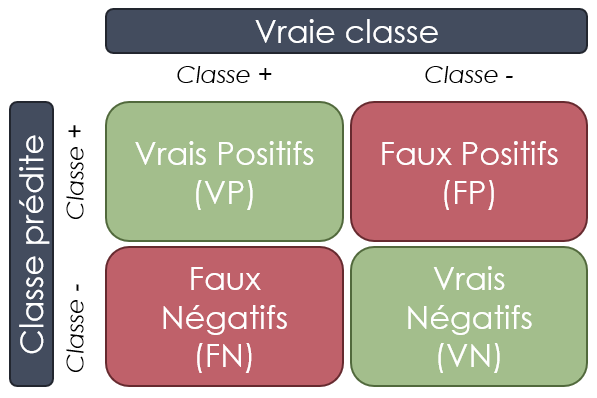
\includegraphics[width=0.5\textwidth]{figures/confusion_example.png}
 \caption[Exemple de matrice de confusion binaire]{Exemple de matrice de confusion binaire}
 \label{fig:confusion-example}
\end{figure}

\subsubsection{Exactitude}
L'exactitude est une mesure de performance classique qui évalue la proportion de points de données correctement classées par rapport aux nombres totaux de points de données. Cette mesure est trompeuse dans le cadre de données déséquilibrées. Elle est calculée telle que :
\[ \text{Exactitude} = \frac{\text{Vrais Positifs} + \text{Vrais Négatifs}}{\text{Vrais Positifs} + \text{Vrais Négatifs} + \text{Faux Positifs} + \text{Faux Négatifs}} \]

\subsubsection{Exactitude équilibrée}
L'exactitude équilibrée quant à elle est utile dans le cadre d'un jeu de données déséquilibré. Elle donne une importance égale aux performances de chaque classe. Pour cela, la sensibilité (ou rappel, c'est-à-dire le nombre de bonnes prédictions pour une classe sur l'ensemble des membres de la classe) est calculée pour chaque classe. Ensuite, l'exactitude équilibrée correspond donc à la moyenne de la sensibilité pour chaque classe. Ainsi sa formule est égale à :
\[ \text{Exactitude équilibrée} = \frac{1}{n} \sum_{i=1}^{n} \text{Exactitude}_i \] où n représente le nombre de classes différentes.

\subsubsection{Précision, sensibilité, spécificité et Score F1}
La figure \ref{fig:prec_recall_spec} présente les notions de précision, sensibilité (rappel) et spécificité en prenant comme exemple l'interprétation d'un test COVID. Pour un test COVID, la précision représente la proportion de patients réellement positifs parmi des tests positifs. Le sensibilité (ou rappel) représente la proportion de tests positifs parmi l'ensemble des personnes positives à la COVID. Enfin la spécificité mesure la proportion de tests réellement négatifs parmi l'ensemble des patients négatifs au COVID.

\begin{figure}[!ht]
 \centering
 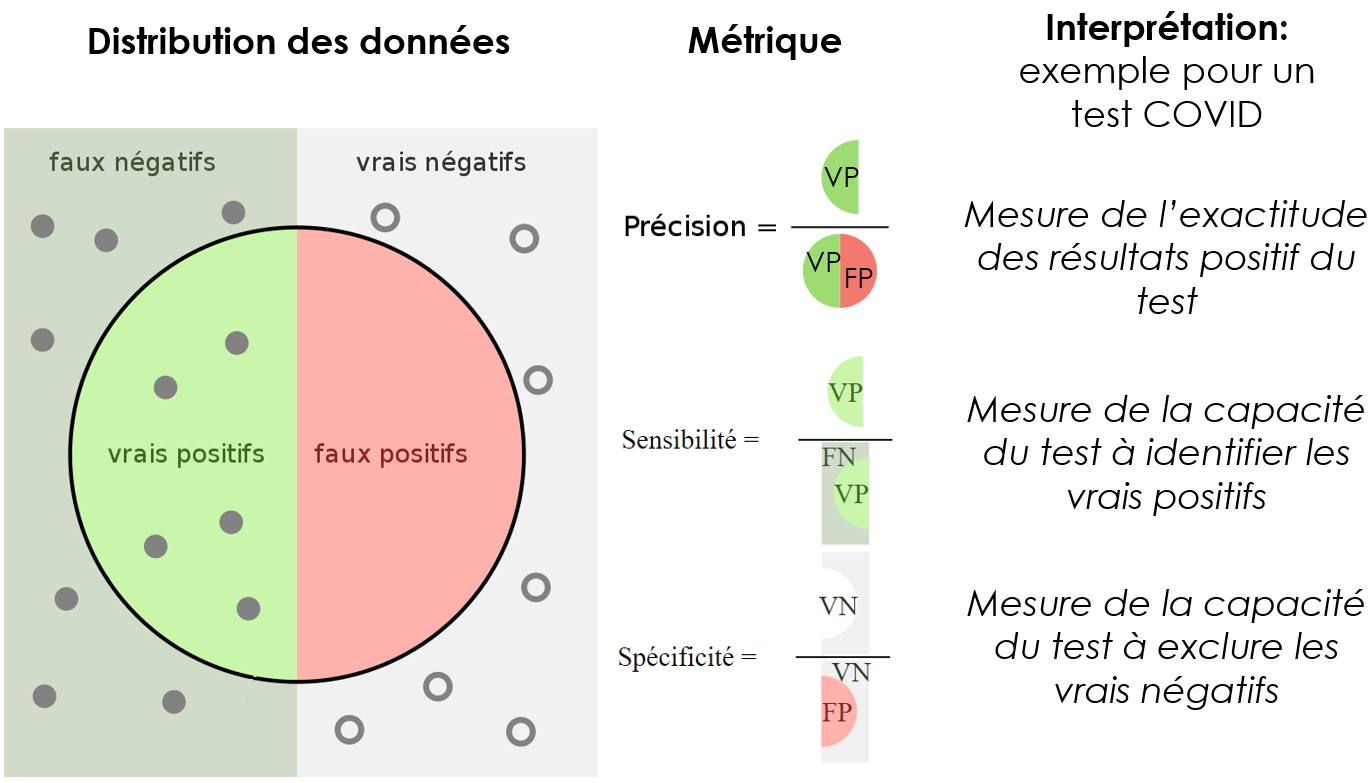
\includegraphics[width=1\textwidth]{figures/prec_recall.png}
 \caption[Précision, sensibilité et spécificité]{Schéma de la notion de précision, sensibilité et spécificité (modifié de Wikipédia "Précision et rappel")}
 \label{fig:prec_recall_spec}
\end{figure}

Le score-F1 correspond à la moyenne harmonique de la précision et de la sensibilité (rappel) et donc permet de tenir compte à la fois des faux positifs et des faux négatifs. Dans le cadre de classification multi-classe (3 et plus), le score F1 peut être calculé de plusieurs manières. Soit de manière "micro" c'est-à-dire globalement à partir du nombre de vrais positifs, faux négatifs et faux positifs. Soit de manière "macro", en calculant le score F1 de chaque classe et en réalisant leur moyenne, similairement à la différence entre exactitude et exactitude équilibrée. Ainsi la formule du score F1-Macro est :
\[ \text{Score F1 Macro} = \frac{1}{n} \sum_{i=1}^{n} \frac{2 \times \text{Précision}_i \times \text{Rappel}_i}{\text{Précision}_i + \text{Rappel}_i} \] où \(n\) représente le nombre de classes différentes.

\subsubsection{Coefficient de corrélation de Matthew}
Le \gls{mcc} est une métrique prenant en compte l'ensemble des éléments de la matrice de confusion (vrais positifs, faux positifs, vrais négatifs, faux négatifs), contrairement aux métriques présentées ci-dessus. De plus, elle est équilibrée, c'est-à-dire qu'elle n'est pas biaisée dans le cas de classes déséquilibrées. Ses valeurs sont comprises entre -1 et 1, avec 0 pour des prédictions aléatoires, 1 pour des prédictions parfaites et -1 pour des prédictions parfaitement contraires. Cette métrique est plus informative sur la qualité d'un modèle que le score F1 (\cite{chicco_advantages_2020}). Dans le cadre d'une classification binaire, la formule du MCC est :
\[ MCC = \frac{VP \times VN - FP \times FN}{\sqrt{(VP + FP)(VP + FN)(VN + FP)(VN + FN)}} \]
Dans le cadre d'une classification multi-classe, la formule est plus complexe :
\[ MCC = \frac{
    c \times s - \sum_{k}^{K} p_k \times t_k
}{\sqrt{
    (s^2 - \sum_{k}^{K} p_k^2) \times
    (s^2 - \sum_{k}^{K} t_k^2)
}} \]
où \(c\) représente le nombre d'échantillons correctement prédits, \(s\) représente le nombre total d'échantillons, \(p_k\) le nombre de fois où la classe k a été prédite, \(t_k\) le nombre de fois où la classe k s'est réellement produite.

\section{Techniques d'analyse d'image et réseaux de neurones}
Les méthodes que nous avons développées permettent d'analyser des données d'imagerie histologique. L'outil \gls{impatient} présenté dans le chapitre 5 permet de faire de l'annotation et segmentation d'image en utilisant des techniques d'analyse d'image traditionnelles. L'outil \gls{myoquant} présenté dans le chapitre 8 permet de faire de la quantification de marqueurs pathologiques grâce à la fois à des méthodes d'analyse traditionnelles, mais aussi grâce à des modèles préentrainés et des réseaux de neurones profonds.  Dans cette section nous allons voir les bibliothèques de codes, les modèles et le matériel que nous avons utilisés. 

\subsection{Méthodes d'analyse d'image traditionnelles avec scikit-image}
Pour l'analyse d'image en utilisant des méthodes traditionnelles nous avons utilisé la bibliothèque de code \textit{scikit-image} (\cite{walt_scikit-image_2014}, \href{https://scikit-image.org/}{https://scikit-image.org/}). \textit{Scikit-image} a été développé en 2014 et met à disposition des outils de base pour l'analyse d'image tel que le calcul de contraste, d'intensité et de texture de pixels qui sont des mesures utilisées par \gls{impatient} pour la segmentation d'image. Dans \gls{myoquant}, \textit{scikit-image} est utilisé pour tracer des lignes, réaliser de l'érosion d'image et mesurer des surfaces, périmètres, diamètre de Feret et la position des centroïdes à partir de masques de segmentation.

\subsection{Modèle préentrainé Cellpose et Stardist}
Dans le cadre de \gls{myoquant} nous avons utilisés des modèles préentrainés pour l'analyse des images de coupes histologiques. Pour la segmentation des fibres musculaires, nous avons utilisé l'implémentation Python du modèle Cellpose (\cite{stringer_cellpose_2021}, \href{https://github.com/MouseLand/cellpose}{https://github.com/MouseLand/cellpose}). Parmi les différents modèles inclus dans Cellpose, nous avons utilisé spécifiquement le modèle \textit{cyto2}, qui est le modèle disponible dans Cellpose le plus récent et performant pour la segmentation des fibres musculaires sous diverses colorations. 

Quant à la segmentation des noyaux cellulaires, nous avons utilisé l'implémentation Python du modèle Stardist (\cite{weigert_star-convex_2020}, \href{https://github.com/stardist/stardist}{https://github.com/stardist/stardist}). Plus précisément dans le cadre de l'analyse des noyaux dans la coloration \gls{he}, nous avons utilisé le modèle préentrainé \textit{2D\_versatile\_he}, qui est un modèle spécifiquement entrainé sur des images à la coloration \gls{he}.

\subsection{Développement de réseaux de neurones profond de type ResNet avec Keras Tensorflow}
En plus des modèles préentrainés, dans \gls{myoquant} nous avons entrainé et intégré nos propres modèles de classification basés sur les réseaux de neurones profonds. Pour cela nous avons utilisé les bibliothèques de code Keras (\cite{chollet_keras_2015}, \href{https://keras.io/}{https://keras.io/}) et Tensorflow (\cite{martin_abadi_tensorflow_2015}, \href{https://www.tensorflow.org/}{https://www.tensorflow.org/}). Keras est une bibliothèque qui permet une interaction simplifiée avec Tensorflow mettant à disposition plusieurs architectures de modèles préétablis ainsi que des fonctions permettant d'accélérer le développement de modèles de réseaux de neurones. Dans le cadre de développement de modèles de classification d'image, nous avons utilisé l'architecture RestNet50 version 2 préentrainée sur le jeu de données \textit{ImageNet} implémentée dans Keras. L'architecture ResNet50 (\cite{he_deep_2015}) est un réseau de neurones convolutifs composé de 48 couches convolutives. Ce modèle possède un total de 23 564 800 paramètres. L'entrainement de ce modèle et son inférence sur des données d'imagerie ont été réalisés sur des machines virtuelles de la plateforme SCIGNE Grand-Est équipée de \gls{gpu} RTX 2080 Ti.

\section{Développement d'outils basés sur modèles linguistiques de grande taille}
Les méthodes que nous avons développées (\gls{nlmyo}) pour analyser du texte libre (compte rendu de biopsie) se basent sur les modèles linguistiques de grande taille. Dans cette section, nous détaillons les outils et modèles que nous avons utilisés.

\subsection{Reconnaissance de texte avec Tesseract}
Dans un premier temps, comme la majorité des comptes rendus sont au format PDF il est nécessaire de les convertir en texte. Pour cela, nous avons utilisé des méthodes d'\gls{ocr}. L'outil libre que nous avons utilisé pour cela se nomme Tesseract (\cite{ray_tesseract_2015}) version 5, mise à disposition en novembre 2021. Cet outil est capable de reconnaitre de manière robuste du texte dactylographié dans plus de 100 langues différentes.

\subsection{Modèles linguistiques de grande taille utilisés}
Dans le cadre du développement de \gls{nlmyo} nous avons utilisé 2 \gls{llms} génératifs et 2 \gls{llms} d'embedding. Pour chaque catégorie de \gls{llms} nous avons voulu comparer les résultats issus de modèles provenant de fournisseurs externes (OpenAI) par rapport à des modèles plus petits hébergés localement.

\subsubsection{Modèles génératifs : OpenAI GPT-3.5 et Vicuna-7B}
Un des critères déterminants pour le choix de modèle génératif est les performances du modèle et la taille de contexte. La taille de contexte pour un \gls{llms} représente le nombre de mots qu'il est capable de traiter lors d'une requête. Ainsi plus la taille de contexte est grande, plus il est possible d'analyser un document de grande taille avec des instructions détaillées. Par exemple, le modèle GPT-3.5-turbo d'OpenAI a une taille de contexte de 4096 jetons, ce qui représente environ 3000 mots en anglais. 

La grande majorité des modèles open source et autohébergeable ont une taille de contexte de 512, ce qui limite leur utilisation pour l'analyse de grands documents. Notre choix de modèle autohébergeable s'est porté sur le modèle Vicuna-7B-1.1 (\cite{chiang_vicuna_2023}, \href{https://huggingface.co/vicuna/ggml-vicuna-7b-1.1}{https://huggingface.co/vicuna/ggml-vicuna-7b-1.1}), qui en plus d'être un modèle de petite taille (7 milliards de paramètres par rapport aux 175 milliards de paramètres de GPT-3.5-turbo) donc facilement hébergeable, possède une taille de contexte de 2048. De plus ce modèle est actuellement le plus  performant parmi les modèles open source de taille 7B (\cite{hendrycks_measuring_2021}). 

Concernant le modèle provenant d'un fournisseur externe, nous avons choisi d'utiliser GPT-3.5-turbo d'OpenAI, car ce modèle allie à la fois une  grande taille de contexte de 4096, d'excellentes performances (4e modèle le plus performant toutes catégories confondues \cite{lianmin_zheng_chatbot_2023}) et possède une \gls{api} accessible à bas coût (0,002 \$ par tranche de 1000 \textit{tokens}).

Pour finir, pour les deux modèles génératifs, nous avons mis le paramètre de température le plus proche de 0 possible, c'est-à-dire à 0,01. Le paramètre de température contrôle le niveau de hasard des réponses du modèle. Plus ce paramètre est proche de 0, plus la réponse du modèle est déterministe. Plus cette valeur est supérieure à 1, plus la sortie est aléatoire. La valeur par défaut du modèle est 1. Ainsi en mettant ce paramètre très proche de 0, les résultats sont reproductibles. 

\subsubsection{Modèle d'\textit{embedding} : OpenAI et Instructor}
Les \gls{llms} d'embedding sont des modèles qui transforment du texte en vecteur numérique, ce qui permet de faire de la classification, du clustering et de la recherche de similarité. Ces modèles sont utilisés dans \gls{nlmyo} pour faire de la prédiction de diagnostic et pour créer un moteur de recherche de patients.

Comme pour les modèles  génératifs, nous avons utilisé deux modèles, un par un fournisseur externe et un autohébergé pour comparer les performances. En termes de choix de modèles, pour le modèle issu de fournisseurs externes, nous avons utilisé le modèle d'\textit{embedding} nommé text-embedding-ada-002, car nous utilisons déjà le modèle génératif du même fournisseur (OpenAI). De plus ce modèle est multilangue et performant, car il est classé 6e en termes de performances d'\textit{embedding} sur 75 modèles testés à travers un panel de 56 jeux de données (\cite{muennighoff_mteb_2022}).

Concernant le modèle autohébergé, nous avons choisi d'utiliser le modèle nommé Instructor (\cite{su_one_2023}, \href{https://huggingface.co/hkunlp/instructor-large}{https://huggingface.co/hkunlp/instructor-large}). Ce modèle est parmi les plus performants, classé 2e sur 75 modèles testés (\cite{muennighoff_mteb_2022}), de plus il comporte dans son jeu d'entrainement des données issues de textes médicaux, ce qui permet d'espérer de bonnes performances pour nos comptes rendus de biopsies. 

\subsection{Interaction avec les modèles linguistiques de grande taille avec LangChain}

Face à la diversité des \gls{llms} génératifs, \gls{llms} d'\textit{embedding} et des outils associés, il est nécessaire d'avoir un outil qui uniformise la façon d'interagir avec ces modèles. C'est l'objectif de la bibliothèque de code nommée LangChain (\cite{chase_harrison_langchain_2022}) que nous avons utilisé à travers \gls{nlmyo}. Cette bibliothèque de code permet d'unifier la façon d'interagir avec les modèles autohébergés et les différents fournisseurs externes, ce qui permet d'accélérer la phase d'exploration des performances des modèles et le développement d'outils basés sur les \gls{llms}. 

En plus des interactions avec les modèles de langage, LangChain met à disposition des outils pour interagir avec des bases de données optimisées pour le stockage et la requête de vecteurs numériques (résultats des modèles d'\textit{embedding}). Ainsi dans \gls{nlmyo} nous avons utilisé la base de données de vecteurs nommée ChromaDB (\href{https://www.trychroma.com/}{https://www.trychroma.com/}). Les bases de données de vecteurs sont des bases de données qui permettent de stocker des documents ainsi que leurs résultats d'\textit{embedding}. Ces bases sont optimisées pour le calcul de similarité entre un vecteur requête et une grande base de données de vecteurs. Cela permet par exemple de construire des moteurs de recherche de documents, dans notre cas il s'agit d'un moteur de recherche de comptes rendus de biopsie requêtables par symptômes.

\section{Développement d'outils et d'interfaces}
Les divers outils que nous avons développés dans cette thèse (\gls{impatient}, \gls{nlmyo}, \gls{myoquant}) sont disponibles sous différentes formes : applications web complètes, démonstrations en ligne, outils en ligne de commande.  Pour cela, nous avons utilisé diverses bibliothèques de code spécifique à chaque cas de figure.

\subsection{Développement d'une application web complète pour IMPatienT}
Dans le cadre du développement de notre application web et base de données \gls{impatient} nous avons entièrement construit une application web de zéro. Les applications web sont composées de trois éléments : l'interface (nommée \textit{front-end}), le serveur de calcul (nommé \textit{back-end}) et la base de données. Pour construire l'interface de \gls{impatient}, nous avons utilisé la bibliothèque de code graphique CSS BootStrap (\cite{mark_otto_bootstrap_2011}) couplée à la bibliothèque de code JavaScript JQuery (\cite{resig_jquery_2006}) pour l'interactivité du site. Concernant la partie serveur, nous avons utilisé la bibliothèque de code Python nommée Flask (\cite{ronacher_flask_2010}).  Nous avons utilisé Flask car c'est une bibliothèque minimaliste et bien documentée qui permet de construire un site web rapidement en augmentant graduellement la complexité. Enfin, en guise de base de données, nous avons utilisé le système de base de données relationnelle SQLite \cite{hipp_sqlite_2020}. Le système SQLite a l'avantage d'être léger et portable, car la base de données n'est composée que d'un seul fichier tout en proposant presque les mêmes fonctionnalités que les systèmes de base de données relationnelles plus complexes.

\subsection{Développement d'un outil en ligne de commande pour MyoQuant}
Dans le cadre du développement de notre outil d'analyse d'images \gls{myoquant}, nous avons décidé de rendre l'outil disponible d'abord sous la forme d'outil en ligne de commande. En effet, comme \gls{myoquant} est voué à analyser des images de grande taille pendant des temps d'analyse longs et sur des ordinateurs avec de l'équipement spécialisé, l'outil en ligne de commande semble être la modalité la plus adaptée. Pour cela nous avons utilisé les bibliothèques de code python nommées Typer (\cite{ramirez_typer_2019}) et Rich (\cite{will_mcgugan_rich_2020}). Typer permet de créer des commandes complexes pour un outil en ligne de commande, de valider les paramètres et de générer automatiquement la documentation nécessaire à l'outil, tandis que Rich permet d'enrichir l'expérience de l'usage de la ligne de commande en affichant des données formatées directement dans le terminal (en couleur, sous forme de tableau, interactives etc.).

\subsection{Développement de démonstrations en ligne pour NLMyo et MyoQuant}
Enfin, pour le développement de \gls{nlmyo} mais aussi pour \gls{myoquant} nous avons voulu développer des applications de démonstration en ligne. Ces applications de démonstration ont pour but de faciliter la communication autour des outils et de pouvoir démontrer leur utilité. Pour cela nous avons utilisé la bibliothèque de code Python nommée Streamlit (\cite{adrien_treuille_streamlit_2018}). Streamlit permet de construire des applications web simples et interactives très rapidement sans avoir à gérer la partie interface et serveur séparément, le tout dans un seul et même langage de programmation. L'utilisation de Streamlit nous a permis de mettre en place, de modifier et d'affiner rapidement des démonstrations de nos outils basés sur l'IA.

\section{Recherche ouverte et reproductibilité}
La recherche ouverte est essentielle, notamment en \gls{ia} pour faciliter l'adoption des outils, les améliorer et permettre leur analyse critique. Dans cette optique de science ouverte, nous avons utilisé différents outils pour partager nos travaux de recherche de façon libre et ouverte et les rendre reproductibles.

\subsection{Développement open source et versionnage avec GitHub}
Le code correspondant à l'ensemble des outils et des travaux présentés dans cette thèse est disponible de façon libre et open source sur mon profil GitHub (\href{https://github.com/lambda-science}{https://github.com/lambda-science}). GitHub est une société fondée en 2008 qui permet le versionnage de code informatique. Le versionnage est un système qui permet de traquer les modifications apportées  au code dans le temps et de garder une trace de toutes les versions qui ont existé. L'utilisation de tels systèmes facilite la collaboration en permettant à n'importe qui de contribuer au code, de proposer des améliorations ou de signaler des problèmes éventuels.

\subsection{Développement de données et modèles IA open source avec HuggingFace}
Si GitHub permet de versionner le code, il est aussi nécessaire d'avoir des outils permettant de rendre public et versionnable les modèles d'\gls{ia} entrainés et les données utilisées. Mettre à disposition les modèles IA et les données utilisées de façon open source permet à la communauté d'évaluer de manière indépendante les modèles, mais aussi de les améliorer en entrainant de meilleurs à partir du jeu de données de base. Pour cela, nous avons mis en ligne les données utilisées pour entrainer le modèle SDH de \gls{myoquant} ainsi que le modèle avec son code d'entrainement sur la plateforme HuggingFace à l'adresse : \href{https://huggingface.co/corentinm7}{https://huggingface.co/corentinm7}. HuggingFace est une société fondée en 2016 qui permet de mettre en libre accès des jeux de données et des modèles d'\gls{ia} de manière open source. De plus, HuggingFace développe de nombreuses bibliothèques de code Python open source spécialisées en \gls{ia} comme la bibliothèque nommée \textit{transformers} qui permet l'entrainement de \gls{llms}.

\subsection{Suivi d'expérience avec \textit{Weight and Biais}}
L'entrainement d'un modèle \gls{ia} est un processus long qui passe par de nombreuses phases de recherche sur les algorithmes et les architectures les plus performantes, les paramètres optimaux ou le meilleur prétraitement des données pour obtenir  un modèle performant. Pour traquer les performances des divers modèles entrainés et les comparer, des outils existent à l'instar de GitHub et HuggingFace. Dans cette thèse j'ai utilisé l'outil nommé \textit{Weight and Bias} (\href{https://wandb.ai/}{https://wandb.ai/}), une société fondée en 2017, pour traquer les performances des divers entrainements des modèles de \gls{myoquant} et \gls{nlmyo}. Dans les chapitres suivants, un lien vers les résultats en ligne est fourni pour accéder à l'ensemble des informations enregistrées.

\subsection{Environnement de développement reproductible}
Le dernier élément concernant la reproductibilité des travaux après avoir fourni le code, les données et les modèles de manière open source reste de s'assurer que le code puisse s'exécuter correctement quel que soit l'environnement informatique. Pour cela, pour chaque outil, nous fournissons deux éléments. En premier nous fournissons un environnement virtuel Python avec Poetry (\href{https://python-poetry.org/}{https://python-poetry.org/}) qui permet de spécifier les versions exactes de bibliothèques de code python utilisées ainsi que les versions de leurs dépendances. De plus, nous construisons une image Docker (\href{https://www.docker.com/}{https://www.docker.com/}) pour chaque outil ce qui permet non seulement de contrôler la version de Python utilisée, mais aussi le système d'exploitation et les versions de ses diverses bibliothèques de codes annexes. L'utilisation d'images Docker couplée à un environnement virtuel Python spécifique permettent de s'assurer que notre code fonctionne et est reproductible sur n'importe quel matériel informatique.

\subsection{Archivage du code, des données et des résultats avec Zenodo}
Zenodo  (\cite{european_organization_for_nuclear_research_zenodo_2013}, \href{https://zenodo.org/}{https://zenodo.org/}) est un outil développé par le \gls{cern} en 2013, qui permet d'archiver des travaux de recherche, du code et des données et d'y associer un identifiant unique citable (\gls{doi}). Dans le cadre de cette thèse, nous avons créé une archive Zenodo qui contient l'ensemble des éléments de cette thèse, c'est-à-dire : le manuscrit, le code des outils, les données non confidentielles utilisées, les modèles entrainés et les résultats. Le lien vers cette archive est \href{LIEN A GENERER}{LIEN A GÉNÉRER}.
\part{CONTRIBUTIONS}
\chapter{Classification des rapports histologiques par IA Explicable (xAI)}
% ...
Placeholder
\chapter{Analyse de la base de données d’IMPatienT par IA Explicable (xAI)}

\section{Contexte}
La création d'un vocabulaire standard décrivant les observations (termes) faites lors de la biopsie musculaire a permis grâce à \gls{impatient} la numérisation de 89 rapports de biopsie de patients atteints de \gls{mc}. Ce tableau de données peut servir de jeu de données pour l'entraînement de modèles \gls{ml} traditionnels pour en évaluer les performances et les comparer aux modèles explicables. C'est précisément l'objet de cette analyse.
\section{Contenu de la base de données}
Chacun des 89 rapports d'histologie ont été numérisés à la main en annotant via \gls{impatient} chacun des termes du vocabulaire entre: absence du terme (0), présence (suivant 4 gradations de quantité de 0.25 à 1) ou absence d'information (N/A).  Cette procédure a permis d'obtenir une matrice numérique de taille (89,175) où les 175 colonnes représentent les 175 termes du vocabulaire standard. De plus, pour chacun des 89 rapports un certain nombre de méta-données ont été enregistrées en plus tel que: l'âge, le numéro de biopsie, le muscle, le diagnostic final, l'identifiant de la biopsie, l'identifiant unique du patient.
\subsection{Analyse statistique exploratoire}
Dans un premier temps j'ai réalisé une analyse statistique exploratoire de ce jeu de données (fig. \ref{fig:impatient_eda}). Ainsi grâce à \gls{impatient} j'ai généré plusieurs visualisation dont des histogrammes, des matrices de corrélations, des tableau de fréquences et des matrice de confusions pour évaluer la méthode \gls{boqa}.  On observe dans notre jeu de données une majorité de patient adultes (49 sur 89). Au niveau des gènes, les gènes TTN, NEB, RYR1 et MYH7 sont les plus souvent responsables de la maladie (40 sur 89). Au niveau diagnostic, les \gls{com} et les \gls{nm} sont les plus communes (28 et 25). Ensuite il y a un grand groupe de patients sans diagnostic clairement établis (23) puis un groupe plus petit de patients à \gls{cnm} (10). Les tableaux des termes les plus fréquents par gène et par diagnostic font ressortir des termes attendues tels que une forte fréquence de bâtonnets sombres dans les \gls{nm}, de noyaux centralisés dans les \gls{cnm} et de cores dans les \gls{com}.
\begin{figure}[htbp]
  \centering
  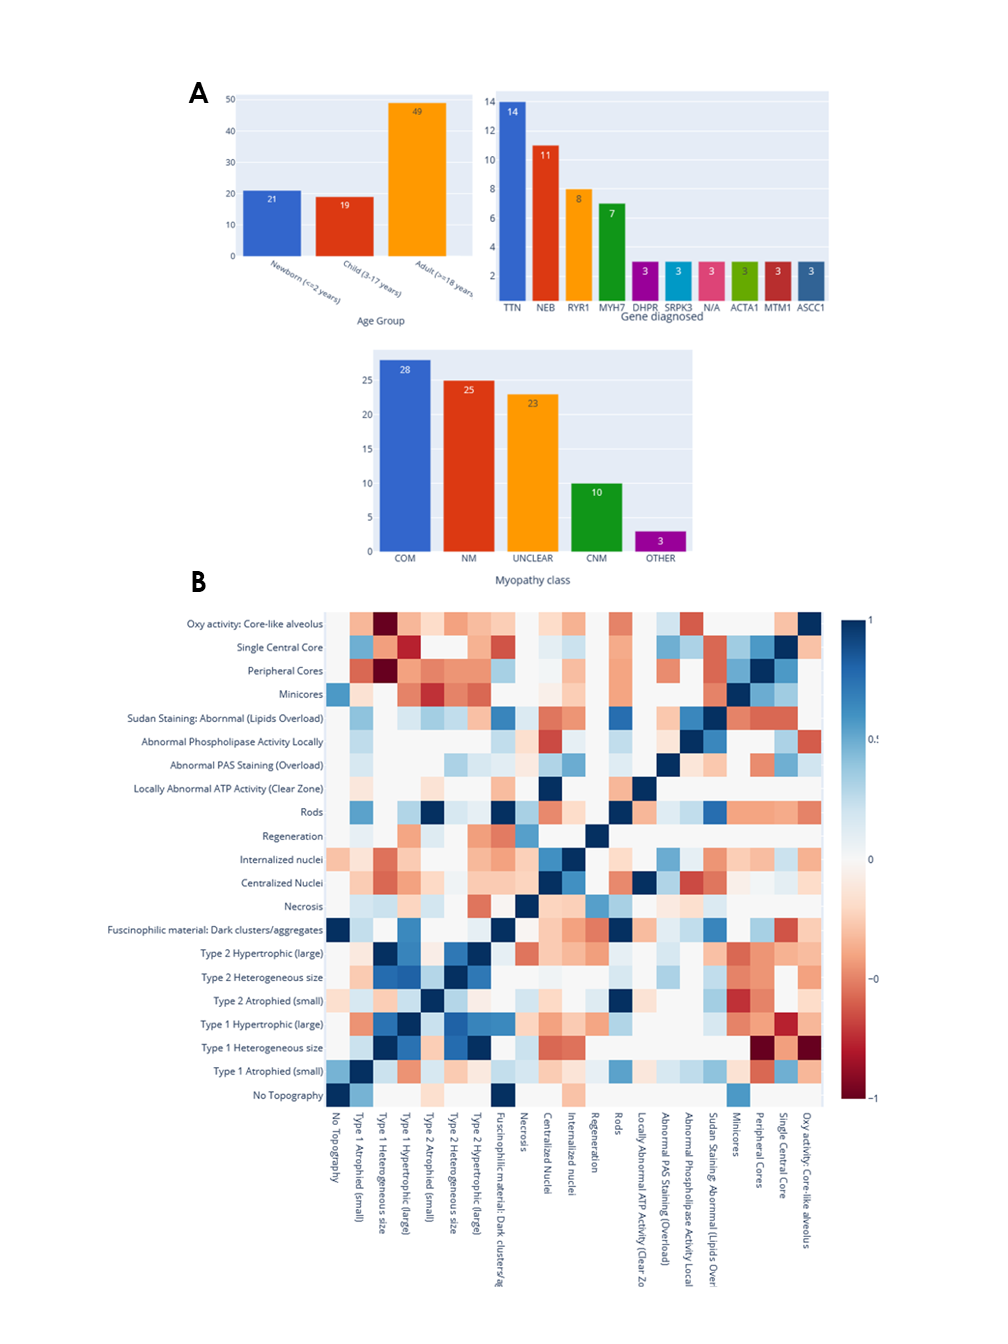
\includegraphics[width=0.98\textwidth]{figures/impatient_explo.png}
  \caption[Analyse statistique exploratoire IMPatienT]{Analyse statistique exploratoire de la base de données IMPatienT. (A) Histogrammes de répartition des patients, (B) Matrice de corrélation des termes du vocabulaire standard.}
  \label{fig:impatient_eda}
\end{figure}
\section{Pipeline de Machine-Learning Streamline}
Nous avons voulu évaluer si il était possible de prédire le diagnostic des patients via des techniques classification par algorithmes de \gls{ml} traditionnels. Pour cela nous avons utilisé et modifié le pipeline Streamline (\cite{urbanowicz_streamline_2022}), développé par \textit{Ryan J. Urbanowicz}, créateur aussi d'un algorithme de classification explicable (de type \gls{lcs})  nommé Exstracs 2.0 (\cite{urbanowicz_exstracs_2015}).
Le pipeline Streamline permet d'entraîner, d'optimiser et de comparer 11 algorithmes traditionnels de \gls{ml} sur un même jeu de données. Ce pipeline est développé pour de la classification binaire, j'ai donc procéder à des modifications pour le rendre compatible avec des tâches de classification multi-classe (prédiction de diagnostic entre les \gls{nm}, \gls{com} et les \gls{cnm}).
\section{Résultats d'analyse}
L'utilisation de Streamline nous a permis de comparer 11 algorithmes de \gls{ml} pour la classification de données biomédicales (table \ref{table:ml_metrics}). Parmi ces 11 algorithmes, 9 ont montré des performances similaires, avec une exactitude de classification se situant entre 0,77 et 0,83. Cependant, les algorithmes eLCS et xLCS ont obtenu des performances nettement inférieures, avec une exactitude de classification de 0,32 et 0,34 respectivement (performances quasi aléatoire). Ces résultats se perçoivent aussi en observant la courbe ROC (fig. \ref{fig:roc_curve}).
\begin{figure}[htbp]
  \centering
  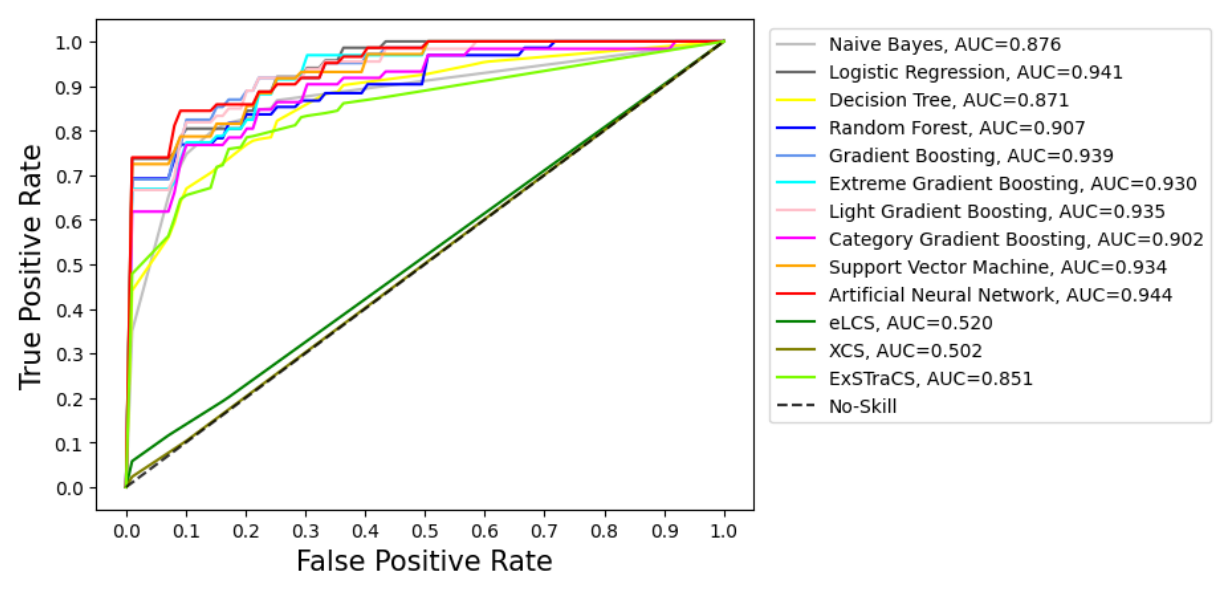
\includegraphics[width=1\textwidth]{figures/roc_streamline.png}
  \caption[Comparaison des courbes ROC]{Comparaison des courbes ROC des 11 algorithmes comparés.}
  \label{fig:roc_curve}
\end{figure}
\begin{table}[htbp]
\centering
\begin{tabular}{lcccc}
\hline
Algorithme & Exactitude Pondérée & Exactitude & Matthew Corr. Coeff. & Spécificité  \\
\hline
Naive Bayesienne & 0.77 & 0.82 & 0.73 & 0.91 \\
Regession Logistique & 0.75 & 0.79 & 0.69 & 0.89 \\
Arbre de décision & 0.72 & 0.77 & 0.62 & 0.86 \\
Random Forest & 0.74 & 0.77 & 0.67 & 0.89 \\
Boosting & 0.81 & 0.82 & \textbf{0.75} & 0.91 \\
XGBoost & 0.72 & 0.77 & 0.66 & 0.89 \\
LGB & 0.73 & 0.80 & 0.71 & 0.90 \\
Cat-Boost & 0.71 & 0.77 & 0.66 & 0.89 \\
SVM & \textbf{0.83} & 0.80 & 0.74 & 0.90 \\
Perceptron & 0.74 & \textbf{0.83} & 0.74 & \textbf{0.92 }\\
eLCS & 0.32 & 0.38 & 0.05 & 0.69 \\
XCS & 0.33 & 0.46 & 0.04 & 0.73 \\
ExSTraCS & 0.68 & 0.77 & 0.65 & 0.89 \\
\hline
\end{tabular}
\caption{Comparaison des performances des modèles (moyenne sur 10 CV)}
\label{table:ml_metrics}
\end{table}        
L'algorithme \gls{svm} s'est révélé être le meilleur algorithme en terme d'exactitude pondérée. En revanche, l'algorithme de système de classeur ExSTraCS 2.0, qui présente l'avantage d'être très explicable, a affiché une performance légèrement inférieure, avec une exactitude de classification de 0,77 (et de 0,68 pour l'exactitude pondérée). Il est intéressant de noter que l'algorithme de classification naïve bayésienne, qui est à la fois simple et par nature explicable, a obtenu des performances similaires à celles de la SVM, tout en ayant un temps d'entraînement faible de 22 secondes en raison de sa simplicité et de l'absence d'hyper-paramètre à optimiser (table \ref{tab:pipeline_times}). A titre de comparaison, le \gls{lcs} ExSTraCS a nécessité un temps d'entraînement de  9 minutes, et ceci sans phase d'optimisation des hyper-paramètres.
\begin{table}[htbp]
    \centering
    \begin{tabular}{lc}
        \toprule
        Algorithme & Temps d'optimisation et d'entraînement (sec) \\
        \midrule
        Naive Bayesienne & 22.89 \\
        Regession Logistique & 61.82 \\
        Arbre de décision & 29.6 \\
        Random Forest & 3325.78 \\
        Boosting & 3078.92 \\
        XGBoost & 1345.9 \\
        LGBoost & 329.61 \\
        Cat-Boost & 6664.66 \\
        SVM & 39.04 \\
        Perceptron & 1391.7 \\
        eLCS & 1909.32 \\
        XCS & 1832.16 \\
        ExSTraCS & 534.56 \\
        \bottomrule
    \end{tabular}
    \caption{Temps d'optimisation et d'entraînement des algorithmes}
    \label{tab:pipeline_times}
\end{table}
\begin{figure}[htbp]
  \centering
  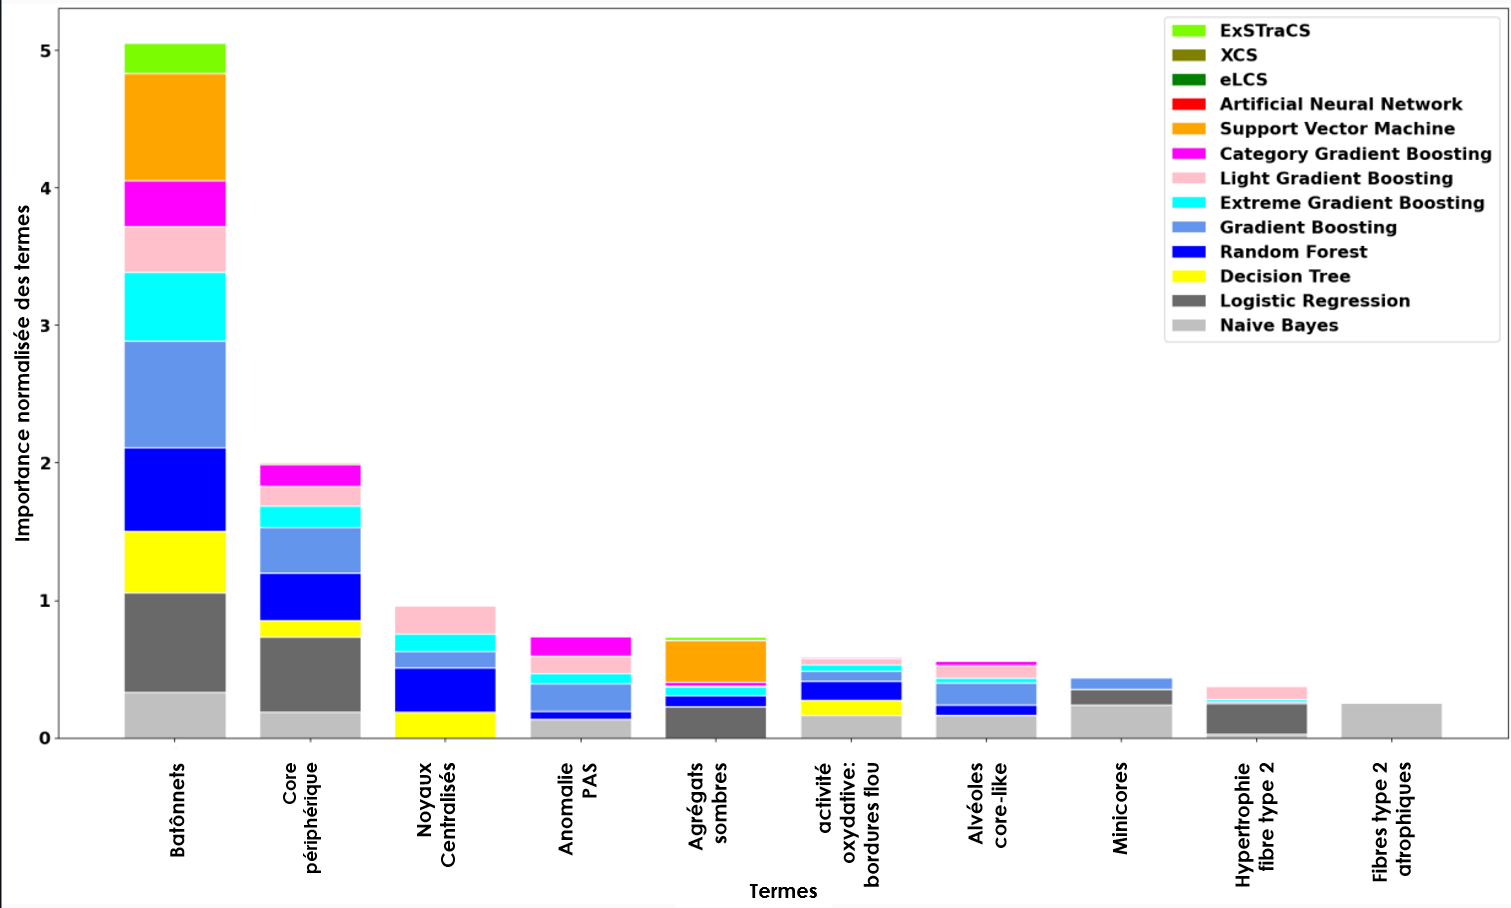
\includegraphics[width=1\textwidth]{figures/feature_importance.png}
  \caption[Histogramme des 10 termes les plus déterminants pour la classification]{Histogramme des 10 termes les plus déterminants pour la classification}
  \label{fig:feautre_importance}
\end{figure}
L'histogramme montrant les 10 termes les plus importants pour la classification dans l'ensemble des algorithmes (fig. \ref{fig:feautre_importance}) met en évidence des termes attendu comme le présence de bâtonnet, de core ou de noyaux centralisés pour faire la différence entre \gls{nm}, \gls{com} et \gls{cnm} avec un poids très important pour la présence de bâtonnets. Mais on observe aussi la présence de critère moins attendu comme la présence d'anomalie au marquage PAS et l'hypertrophie ou atrophie des fibres de type 2.
L'ensemble de ces résultats suggèrent que la taille et l'hétérogénéité du jeu de données pourraient être insuffisantes pour permettre une comparaison des algorithmes. Sur notre jeu de donnée, il semblerait que l'utilisation d'algorithmes simples comme la méthode naïve bayésienne soit à privilégier pour sa triple efficacité en terme de performances, explicabilité et coût en puissance de calcul.  Il est possible que l'utilisation d'un ensemble de données plus important, c'est à dire contenant plus de compte-rendus de biopsie, et homogène permettrait une meilleure évaluation des performances de ces algorithmes et, par conséquent, une meilleure compréhension de leurs avantages et inconvénients respectifs dans le contexte de la classification de données biomédicales de manière explicable.
\section{Méthode de visualisation des règles de LCS}
Les \gls{lcs} produisent une liste de règle pour la classification ce qui peut être difficile à interpréter visuellement. Nous avons voulu explorer différentes approches pour représenter graphiquement ces règles, afin d'extraire des connaissances à partir de cette liste. Le code écrit pour générer ces visualisation est open-source et est disponible dans un répertoire GitHub à l'adresse: \href{https://github.com/lambda-science/PredEx}{https://github.com/lambda-science/PredEx}.
\subsection{Principe général}
Nous avons développé deux approches pour la visualisation des règles générées LCS.
La première approche consiste à visualiser les interactions entre les termes dans les rapports, c'est à dire leur co-occurrence dans les règles générées. Lorsque deux termes apparaissent dans une même règle défini par notre LCS, un lien est tracé entre eux, produisant un diagramme de cordes. Un lien épais entre deux termes indique une co-occurrence importante dans la liste des règles, suggérant une relation étroite entre ces termes (observations pathologiques).
La seconde approche consiste à visualiser les liens entre les termes et les diagnostics. Sur un graphe, chaque noeud circulaire représente un terme, tandis que les noeuds triangulaires représentent les diagnostics. Pour chaque règle, un lien est tracé entre les termes et le diagnostic correspondant. Plus le terme apparaît dans des règles liées à un diagnostic, plus le lien sera épais, indiquant une relation forte entre l'observation et le diagnostic. Les liens sont colorés en rouge ou vert en fonction de l'absence ou la présence du terme menant au diagnostic, respectivement. Par exemple, si toutes les règles liant le terme "cores" aux \gls{nm} stipulent que les cores doivent être absent, alors le lien sera rouge. Si l'observation est liée au diagnostic à la fois en état d'absence et de présence dans des règles différentes, le lien est coloré en jaune, reflétant la complexité de la relation entre l'observation et le diagnostic.
\subsection{Résultats}
La première approche à permis de générer le diagramme de cordes figure \ref{fig:chords}.  Cette figure est disponible de manière interactive à l'adresse \href{https://lbgi.fr/~meyer/chord.html}{https://lbgi.fr/~meyer/chord.html}. Sur cette représentation nous avons filtré les liens pour ne conserver que les liens ayant une valeur supérieure ou égale à 10 (co-occurrence des deux termes dans au moins 10 règles). On observe sur cette figure des interactions complexes et multiples entre les termes sans pouvoir en tirer un signal clair, il n'y a pas de couple de termes bien défini.
\begin{figure}[htbp]
  \centering
  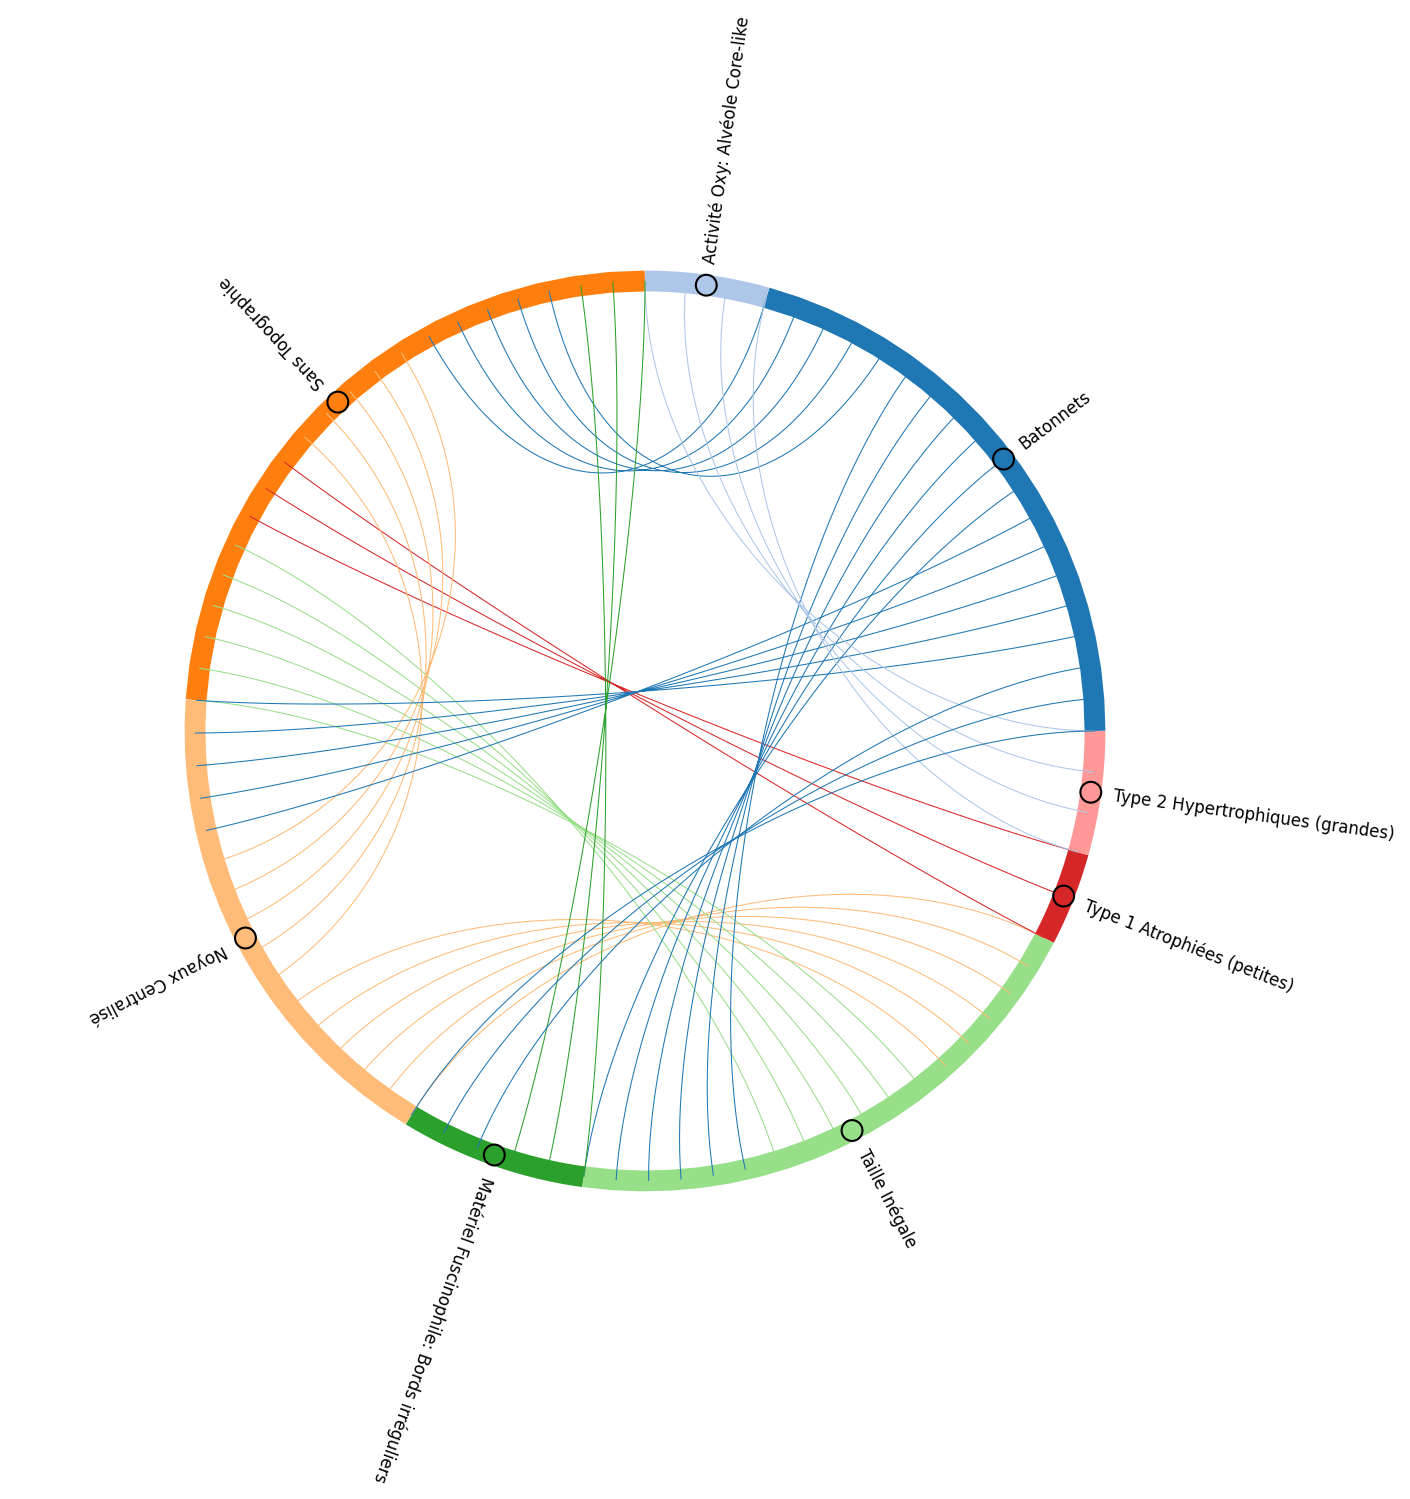
\includegraphics[width=1\textwidth]{figures/chord_plot.png}
  \caption[Diagramme de cordes des règles de LCS]{Diagramme de cordes des règles de LCS}
  \label{fig:chords}
\end{figure}
La seconde approche a permis de générer le réseau représenté dans la figure \ref{fig:network}. Cette figure est disponible de manière interactive à l'adresse \href{https://lbgi.fr/~meyer/myomap.html}{https://lbgi.fr/~meyer/myomap.html}. On observe sur cette représentation qu'une majorité des règles dans notre \gls{lcs} servent à essayer de différencier les \gls{cnm} du reste (de nombreux liens épais). Aussi, on observe que notre LCS essaie de différencier les \gls{cnm} principalement par l'absence de terme (majorité de liens rouges). Ces résultats supposent que l'algorithme parvient facilement à séparer les \gls{nm} des \gls{com} avec un faible jeu de règles, mais la tâche est plus compliquée pour les \gls{cnm}, pour lesquelles il génère un nombre important de règles. On retrouve sur ce réseau, des observations attendues comme la présence d'un lien vert entre \gls{nm} et le terme "bâtonnets", la présence d'un lien vert entre \gls{com} et le terme "cores", et la présence d'un lien vert entre \gls{cnm} et le terme "noyaux centralisés". On observe cependant aussi des critères de classification moins connus comme la présence de bords arrondis pour les fibre musculaire lié de façon positive au diagnostic \gls{cnm} et de façon négative au diagnostic \gls{nm}. Ou encore la présence d'anomalie de coloration PAS associée de façon positive aux \gls{nm} et négative aux \gls{cnm}. L'importance de la coloration PAS pour la classification a déjà été mise en évidence dans l'histogramme de l'importance des termes pour la classification présenté plus haut (fig. \ref{fig:feautre_importance}).
\begin{figure}[htbp]
  \centering
  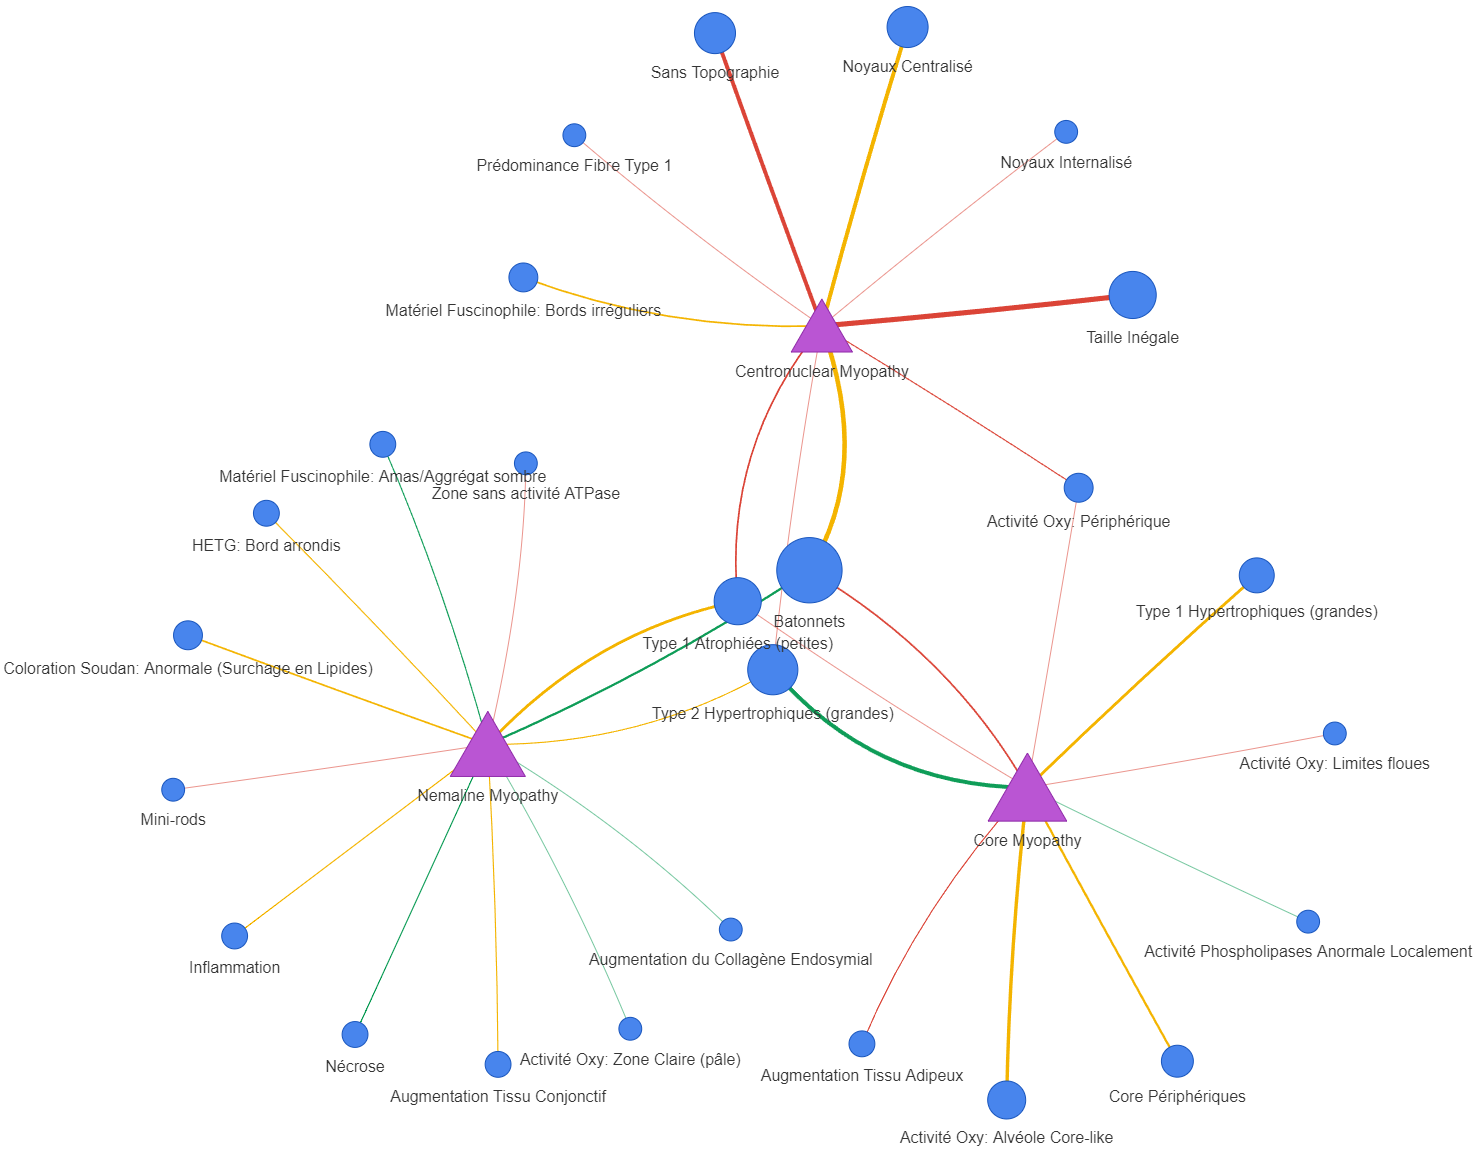
\includegraphics[width=1\textwidth]{figures/network_lcs.png}
  \caption[Représentation des règles de LCS sous forme de réseau]{Représentation des règles de LCS sous forme de réseau}
  \label{fig:network}
\end{figure}
\section{Perspectives de développement}
En terme développement futur, il est nécessaire d'agrandir le jeu de données utilisé pour comparer les algorithmes de classification. En effet, notre jeu de données de 89 rapports semble trop hétérogène et de trop petite taille pour déceler une différence de performances significative entre les algorithmes. De plus, il est nécessaire d'améliorer les approches de visualisation des règles de \gls{lcs}, car ces approches semblent être intéressantes pour visualiser graphiquement et rapidement le fonctionnement interne de notre système de classification explicable et pour identifier de nouveaux critères pertinent pour différencier les sous-types de myopathies congénitales.

Enfin il pourrait être intéressant d'intégrer ce pipeline d'entraînement et ces visualisations à \gls{impatient} pour entraîner automatiquement un modèle de classification performant lors de l'entrée de nouveaux patient. Ce modèle peut être mis à disposition ensuite dans le formulaire d'entrée pour réalise de l'aide au diagnostic.
\chapter{NLMyo : Traitement de rapports textuels par LLMs}

Dans les deux précédents chapitres, nous avons présenté \gls{impatient} un outil d'annotation et d'exploration de compte rendu de biopsie en texte libre. \gls{impatient} utilise un système à base d'ontologie et de vocabulaire standard pour détecter et annoter la présence ou l'absence d'éléments pathologiques dans les biopsies musculaires. Cependant, ce système présente certaines limites. Tout d'abord, il requiert de créer un vocabulaire standard exhaustif pour décrire les observations dans les biopsies musculaires, ce qui est un travail manuel important. De plus, le système d'annotation semi-automatique utilise un système à base de règles et de correspondance exacte des mots aux ontologies existantes. Cette correspondance exacte réduit la flexibilité du système et sa sensibilité de détection, il faut alors réaliser un travail d'annotation manuel important pour numériser les comptes rendus de biopsie. 

En fin 2022 et début 2023, les récentes avancées dans le domaine du \gls{nlp} ont permis de révolutionner la manière de traiter et d'exploiter les données sous forme de texte libre. La mise à dispositions de modèles linguistiques de grande taille (\gls{llms}, \ref{chap2_llms}) performants, accessibles et capables de suivre des instructions, ouvre la porte à la création d'outils plus performants et flexibles pour le traitement de ces comptes rendus. Ces systèmes basés sur une approche sémantique et multilingue éliminent la nécessité de définir un vocabulaire standard. Ainsi nous avons développé \gls{nlmyo} (fig \ref{fig:nlmyo_logo}), une boite à outils basée sur les \gls{llms} mettant à disposition quatre outils généralistes pour le traitement de comptes rendus médicaux: outil d'anonymisation, d'extraction d'information, de classification automatique et de création de moteurs de recherche. L'ensemble de ces outils et des modèles utilisés est représenté dans la figure \ref{fig:nlmyo_struct}.
\begin{figure}[!ht]
 \centering
 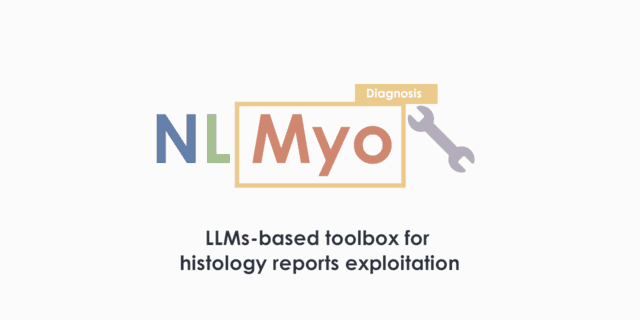
\includegraphics[width=0.5\textwidth]{figures/nlmyo_banner.png}
 \caption[Logo NLMyo]{\textbf{Logo de NLMyo}}
 \label{fig:nlmyo_logo}
\end{figure}
\begin{figure}[!ht]
 \centering
 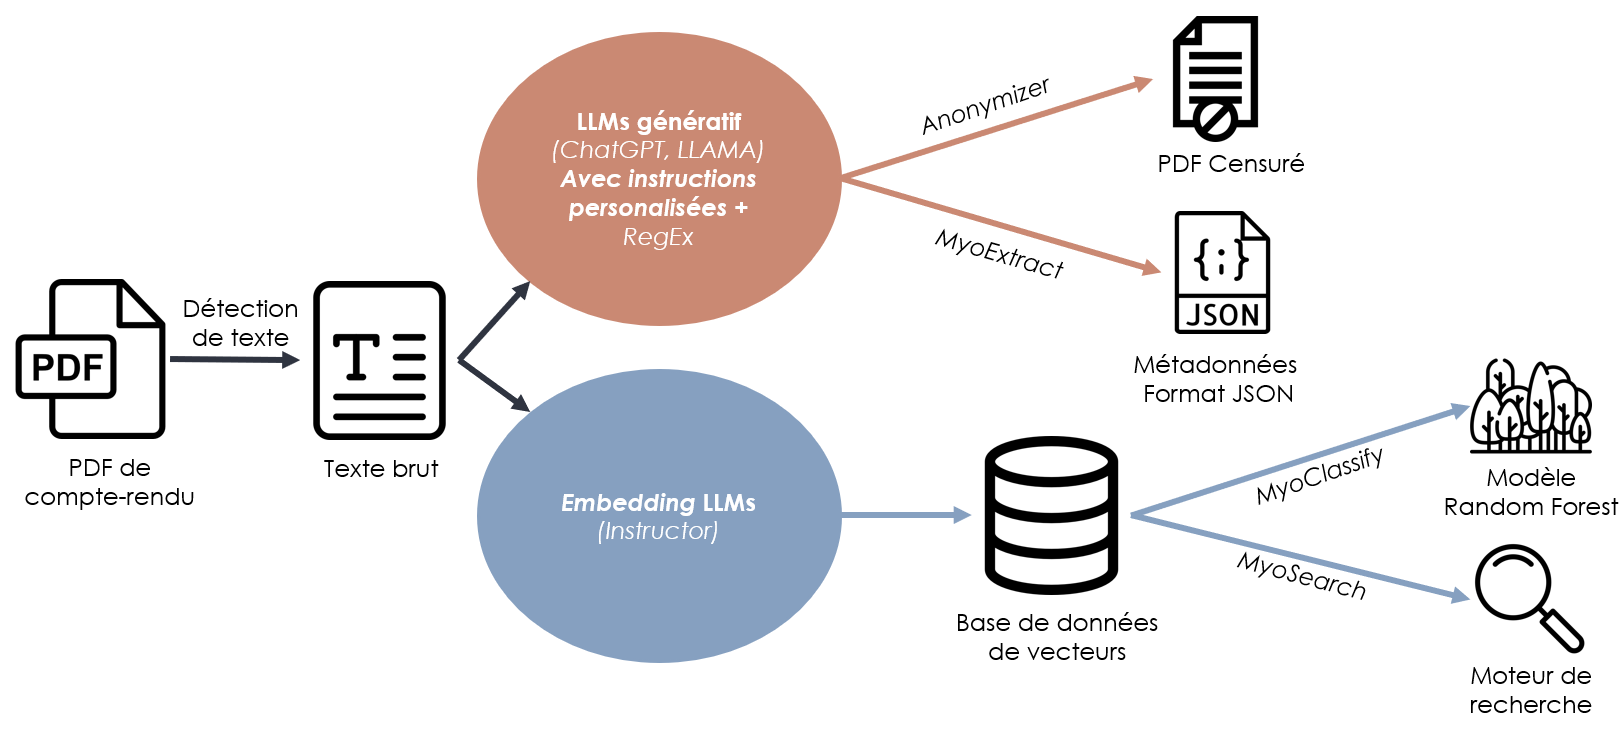
\includegraphics[width=1\textwidth]{figures/nlmyo_struct.png}
 \caption[Structure de NLMyo]{\textbf{Structure de NLMyo}. NLMyo utilise deux types de LLMs pour traiter les comptes rendus de biopsie: les modèles génératifs et les modèles d'\textit{embedding}. L'utilisation de ces deux types de modèles permet la mise à disposition de quatre outils: Anonymizer, MyoExtract, MyoClassify et MyoSerach.}
 \label{fig:nlmyo_struct}
\end{figure}
\section{\textit{Anonymizer}: un outil d'anonymisation}
Le premier outil de \gls{nlmyo} est \textit{Anonymizer}, un outil permettant de supprimer automatiquement les informations identifiantes des comptes rendus médicaux. Dans les comptes rendus de biopsie de l'Institut de Myologie de Paris que nous traitons, deux données identifiantes et personnelles sont présentes et doivent être retirées: le nom du patient (et du personnel médical) ainsi que la date de naissance du patient. Non seulement ces informations ne sont pas utiles pour les analyses subséquentes, mais de plus, par respect de la vie privée et des recommandations \gls{rgpd}, ces informations ne doivent être accessibles qu'aux professionnels en charge du patient. L'anonymisation des rapports est donc une étape essentielle avant le transfert des données, leur numérisation et leur analyse.

Afin de traiter un grand volume de rapports et d'éliminer le travail manuel nécessaire, nous avons tenté d'automatiser la tâche d'anonymisation \textit{via} deux approches: une approche traditionnelle par\gls{regex} et une approche novatrice par\gls{llms}.

\subsection{Anonymisation par RegEx}
En première intention, nous avons développé une méthode basée sur les \gls{regex} pour leur simplicité de mise en place et leur rapidité d'exécution (coûts en puissance de calcul faible). Les \gls{regex} sont des séquences de caractères capables de trouver des motifs dans un texte, par exemple toutes les lignes commençant par "Nom: ". Le tableau \ref{tab:regex} liste les \gls{regex} utilisées pour capturer les informations de noms et de dates. Les comptes rendus de biopsie sont semi-structurés. Pour la plupart, le nom du patient est facilement identifiable, car il est précédé par le préfixe: "Nom: ". Ceci est facilement représenté par la première \gls{regex} listée dans le tableau. Ensuite pour les autres cas de figure, comme les noms de famille sont souvent en majuscule et les prénoms commencent souvent par une majuscule, nous avons développé deux autres \gls{regex} pour capturer les couples de mots dont un est en majuscule et le second commence par une majuscule (ou inversement, lignes 2 et 3 du tableau). 
Ensuite, une troisième \gls{regex} a été ajoutée pour détecter les dates au format JJ-MM-AAAA ou JJ.MM.AAAA (ligne 3 du tableau). Finalement, une dernière \gls{regex} est utilisée pour essayer de trouver le numéro de biopsie dans le document afin de renommer le fichier avec un nom unique et anonyme (ligne 4 du tableau). 
\begin{table}[!ht]
\centering
\caption[Expressions régulières pour extraire les noms et les dates]{\textbf{Expressions régulières pour extraire les noms et les dates}. Trois expressions régulières sont utilisées pour détecter les noms de patients, une expression pour les dates et une expression pour les numéros de biopsie.}
\label{tab:regex}
\begin{tabular}{|l|l|l|}
\hline
\textbf{Expression régulière} & \textbf{Syntaxe} & \textbf{Exemples d'utilisation} \\ \hline
Nom patient & Nom.*: *([A-Za-zÀ-ÿ- ]+) & Nom : Pierre Laroche \\ \hline
Nom patient 2& (([A-Z][a-zÀ-ÿ-]\{3,\} ?)+ ([A-Z-]\{3,\} ?)+) & LAROCHE Pierre \\ \hline
Nom patient 3 & (([A-Z-]\{3,\} ?)+ ([A-Z][a-zÀ-ÿ-]\{3,\} ?)+) & Pierre André LAROCHE \\ \hline
Date & ([(.]?[0-9]\{1,2\}[./][0-9]\{1,2\}[./][0-9]\{1,4\}[().]?) & 07/04/1994, 07.05.18 \\ \hline
N° Biopsie & ([0-9]\{3,8\}[-/]?[0-9]\{0,3\}) & 7377-07, 1234/56 \\ \hline
\end{tabular}
\end{table}
\begin{figure}[!ht]
 \centering
 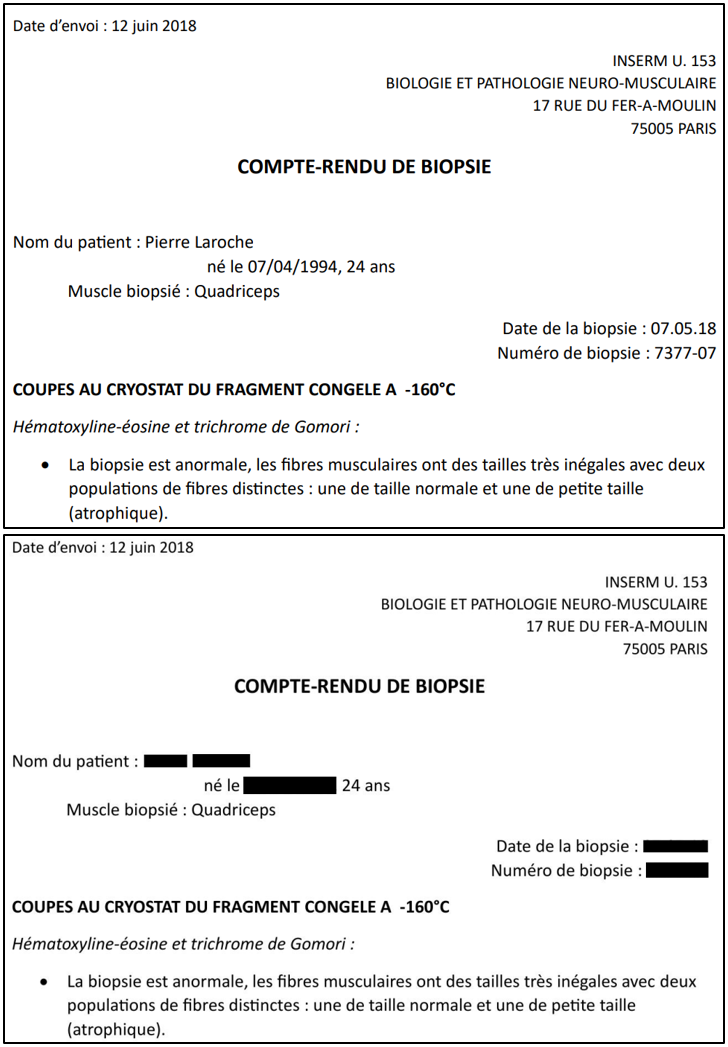
\includegraphics[width=0.8\textwidth]{figures/regex.png}
 \caption[Exemple anonymisation RegEx]{\textbf{Exemple d'anonymisation d'un compte rendus fictif de biopsie avec la méthode RegEx}. En haut le rapport à l'état brut, en bas le rapport censuré. On observe que le nom, le numéro de biopsie et deux dates ont été censurées. Cependant la date d'envoi "12 juin 2018" n'a pas été censurée.}
 \label{fig:regex}
\end{figure}

La figure \ref{fig:regex} présente les résultats de la technique d'anonymisation par \gls{regex} sur l'entête d'un rapport factice de patient, mais avec une structure similaire aux rapports de l'Institut de Myologie de Paris. Les noms et les dates ont été censurés correctement et la méthode a produit de bons résultats. Cependant, cette méthode est insuffisante, car elle est peu sensible (dates ou noms non censurés) et spécifique (informations considérées à tort comme des dates ou des noms). Par exemple tout en haut de l'entête, la date d'envoi "12 juin 2018" n'a pas été censurée. Le tableau \ref{tab:regex_fail} liste trois exemples de cas où cette méthode ne fonctionne pas et produit des erreurs. Il est possible de corriger ces erreurs en augmentant la somme de \gls{regex} utilisées, mais augmenter le nombre de \gls{regex} augmente aussi potentiellement le nombre de faux positifs. De plus, il n'est pas toujours possible de construire une \gls{regex} adaptée pour extraire une information précise. Nous avons alors exploré la capacité des \gls{llms} pour la recherche et l'extraction de ces informations de manière plus robuste et flexible que la méthode \gls{regex}.
\begin{table}[!ht]
\centering
\caption[Exemples de faux positifs ou faux négatifs de la méthode RegEx]{\textbf{Exemples de faux positifs ou faux négatifs de la méthode RegEx}. En fonction du cas de figure, les RegEx peuvent provoquer des faux positifs (censure d'informations excessive) ou des faux négatifs (information personnelle non censurée correctement).}
\label{tab:regex_fail}
\begin{tabularx}{\textwidth}{|l|l|l|X|}
\hline
\textbf{Texte} & \textbf{RegEx déclenchée} & \textbf{Type} & \textbf{Commentaire} \\ \hline
\textit{PAS Staining} & Nom patient 3 & Faux Positif & Nom de coloration dont la notation est confondue avec le motif "NOM Prénom" \\ \hline
\textit{Louis C. Dupont} & N/A & Faux Négatif & La présence du "C." au centre ne permet pas aux RegEx de nom de se déclencher \\ \hline
\textit{12 mars 2001} & N/A & Faux Négatif & La notation de date avec un mois en lettres ne permet pas à la RegEx de date de se déclencher \\ \hline
\textit{1996-04} & N° Biopsie & Faux Positif & La notation de date AAAA-MM déclenche la \gls{regex} de numéro de biopsie. \\ \hline
\end{tabularx}
\end{table}

\subsection{Anonymisation par LLMs}
Les \gls{llms} sont basés sur la compréhension du sens sémantique du texte tandis que les \gls{regex} sont basées sur le principe de motifs de caractères et donc sur la structure du document. L'idée de l'anonymisation par \gls{llms} est d'utiliser un modèle génératif auquel on fournit une instruction et le texte à anonymiser. L'instruction liste les informations à extraire du texte et spécifie le format de sortie. Pour intégrer ces modèles génératifs à outil d'anonymisation, nous voulons récupérer les informations extraites dans un format exploitable informatiquement, nous avons utilisé le format JSON. Le format JSON représente un dictionnaire informatique qui est utilisable par l'application pour censurer les PDF à partir des informations détectées.

\subsection{Instruction personnalisée et \textit{one-shot learning}}
Nous avons construit une instruction personnalisée en 3 parties qui intègre une méthode de \textit{one-shot learning}. Le \textit{one-shot learning} est une technique d'apprentissage qui vise à généralisation en ne donnant qu'un seul exemple d'apprentissage au modèle pour la l'apprentissage d'une nouvelle tâche. Dans l'instruction les trois parties sont: (i) la description de la tâche à effectuer (ii) un exemple de réalisation de la tâche \textit{(one-shot learning)}, (iii) le texte d'intérêt à anonymiser.
Voici un exemple d'instruction que nous utilisons pour réaliser l'extraction des noms et des dates dans les rapports:
\begin{quote}
Tu es un assistant qui extrait des informations d'un texte libre. Le format de ta réponse doit être un format JSON valide qui respecte le nom des clés fournies. Si une valeur est manquante, indique simplement N/A, n'essaie pas d'inventer. Voici la liste des informations à récupérer, les clés JSON sont indiquées entre parenthèses : nom complet (name), dates (date).

ENTRÉE :

Kendrick Lamar et Jane Clinton sont asymptomatiques. Date de naissance : 16 février 1991, numéro de biopsie : 666-77. Ce rapport a été expédié le 01.04.1991.

SORTIE :

\{"name" :["Kendrick Lamar", "Jane Clinton"], "date" : ["16 février 1991", "01.04.1991"]\}

ENTRÉE :

<texte à analyser>

SORTIE :
\end{quote}

La partie précédant le mot clé "ENTRÉE" correspond à l'instruction décrivant précisément la tâche que le modèle doit réaliser (liste des informations à extraire, format de sortie et comportement attendu). Le premier couple "ENTRÉE" et "SORTIE" correspond à un exemple de réalisation de la tâche, ce qui permet de spécifier le schéma JSON attendu au modèle (\textit{one-shot learning}). Puis le second couple "ENTRÉE", "SORTIE" correspond à l'endroit où l'on injecte notre texte d'intérêt à analyser et spécifie au modèle que l'on attend maintenant une sortie textuelle au format JSON pour l'entrée précédente.

\subsection{Exemple et comparaison à la méthode RegEx}
\begin{figure}[!ht]
 \centering
 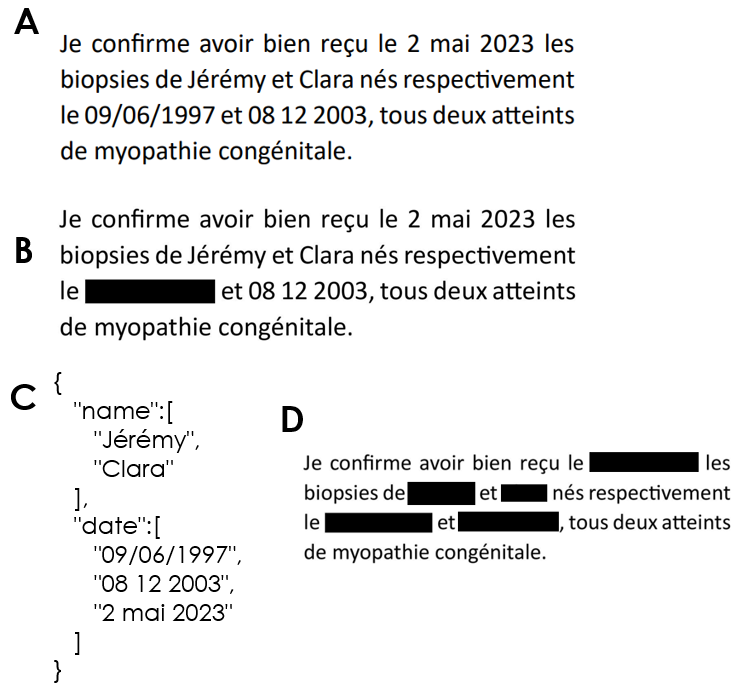
\includegraphics[width=0.8\textwidth]{figures/llms_anonym.png}
 \caption[Exemple anonymisation LLMs]{\textbf{Exemple d'anonymisation d'un courrier médical factice avec la méthode par LLMs}. \textbf{(A) }Texte brut, \textbf{(B)} Anonymisation par RegEx, \textbf{(C) }JSON brut généré par le \gls{llms} GPT-3.5-turbo (OpenAI), \textbf{(D)} Anonymisation à partir du JSON généré par \gls{llms}.}
 \label{fig:llms_anonym}
\end{figure}

Dans cet exemple (figure \ref{fig:llms_anonym}), nous avons construit un début de courrier médical factice faisant figurer des informations personnelles qui ne sont pas détectables par la méthode \gls{regex}. Les prénoms "Jérémy" et "Clara", ainsi que les dates "2 mai 2023" et "08 12 2003" n'ont pas été détectées par la méthode \gls{regex} et n'ont pas été censurées. On observe par contre que la méthode par \gls{llms} (C et D) a été capable d'identifier ces informations et de les extraire du texte. Cet exemple montre que les \gls{llms} peuvent être la base d'un système d'anonymisation plus flexible et moins dépendant de la structure du document.

\section{\textit{MyoExtract}: un outil d'extraction d'information}
À partir des résultats encourageants obtenus avec la technique d'anonymisation par LLMs pour l'extraction d'information, nous avons voulu étendre le champ des informations extraites de manière automatique à partir de texte libre. Nous avons utilisé la même stratégie d'extraction d'information, c'est-à-dire l'utilisation de \gls{llms} génératifs, mais avec une instruction légèrement différente. Cette fois-ci, nous avons ajouté une liste plus importante d'informations à extraire dans le but d'en extraire les métadonnées commune à tout les comptes-rendus de biopsie. Par exemple, nous avons cherché à extraire: les noms, date de naissance, date d'envoi de la biopsie, numéro de biopsie, muscle prélevé, diagnostic final. De plus, nous avons cherché à savoir s'il était possible d'extraire les mentions d'anomalie pour certaines colorations telles que la coloration PAS, Soudan, COX, ATP et Phosphorilase. Cette extraction d'information pourrait permettre d'annoter automatiquement les rapports avec une liste d'anomalies détectées pour chaque coloration. De même que précédemment, nous avons construit une instruction personnalisée en 3 parties (description, exemple, texte à analyser).

Voici un exemple d'instruction que nous utilisons pour réaliser l'extraction des métadonnées et d'anomalies générales des colorations à partir de rapports (à noter que l'instruction présentée est en français mais fonctionne pour l'analyse de texte anglais car les modèles génératifs sont multilingues et peuvent utiliser des instructions contenant un mélange de langues):
\begin{quote}
Tu es un assistant qui extrait des informations d'un texte libre. Le format de ta réponse doit être un format JSON valide qui respecte le nom des clés fournies. Si une valeur est manquante, indique simplement N/A, n'essaie pas d'inventer. Formate les dates sous la forme DD-MM-YYYY et convertis les âges en années (0 si inférieur à 1 an). Voici la liste des informations à récupérer, les clés JSON sont indiquées entre parenthèses : nom complet (name), âge (age), date de naissance (birth), date de la biopsie (biodate), date d'envoi de la biopsie (sending), muscle (muscle), numéro de la biopsie (bionumber), diagnostic (diag), présence d'une anomalie dans la coloration du PAS (PAS), présence d'une anomalie dans la coloration Soudan (Soudan), présence d'une anomalie dans la coloration COX (COX), présence d'une anomalie dans la coloration ATP (ATP), présence d'une anomalie dans la coloration Phosphorylase (phospho)

ENTRÉE:

Kendrick Lamar et Jane Clinton ne sont pas asymptomatiques. Date de naissance: 16 février 1991, numéro de biopsie: 666-77. Anomalie forte à la coloration PAS, mais pas d'anomalie à la coloration lipide soudan. Le tableau est révélateur d'une myopathie à némaline.

SORTIE:

\{"name":["Kendrick Lamar", "Jane Clinton"], "age":"N/A", "birth": "16-02-1991", "biodate": "N/A"", "sending": "N/A"", "muscle": "N/A"", "bionumber": "666-77", "diag": "myopathie à némaline", "PAS": "yes", "Soudan": "no", "COX": "N/A", "ATP": "N/A", "phospho": "N/A"\}

ENTRÉE :

<texte à analyser>

SORTIE :
\end{quote}

\subsection{Exemple d'extraction d'information}
Pour cet exemple d'utilisation, nous avons généré un rapport factice de patient avec une structure similaire aux rapports de l'Institut de Myologie de Paris qui reprend des observations typiques trouvées dans les rapports réels de biopsie. Ce rapport est disponible en figure \ref{fig:factice_report}. 
\begin{figure}[!ht]
 \centering
 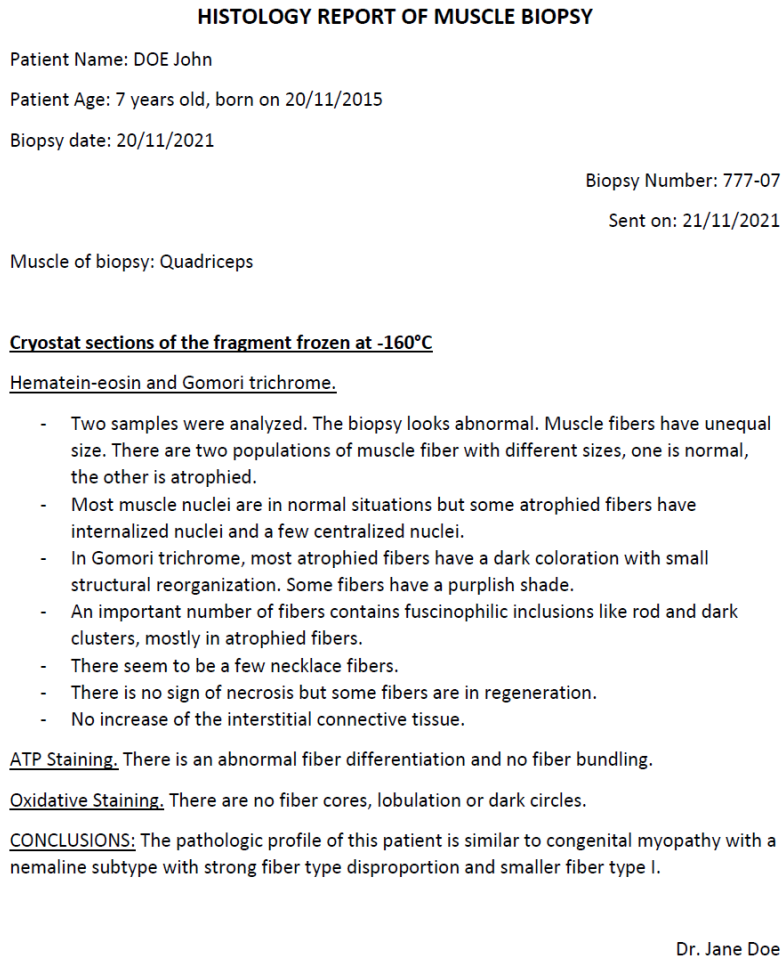
\includegraphics[width=0.85\textwidth]{figures/pdf_biopsie.png}
 \caption[Compte rendus de biopsie fictif]{\textbf{Exemple de compte rendu de biopsie fictif}}
 \label{fig:factice_report}
\end{figure}

Pour extraire les informations, nous avons comparé deux modèles présentés dans le chapitre 4 "Matériels et méthodes": un modèle performant et accessible uniquement via l'\gls{api} commerciale OpenAI (GPT-3.5-turbo) et un modèle autohébergé libre et open source \textit{Vicuna-7B}. Les résultats de l'extraction d'information présentés dans le tableau \ref{tab:json_data} montrent que le modèle d'\textit{OpenAI} GPT-3.5-turbo est capable d'extraire l'ensemble des informations demandées de manière satisfaisante sans erreurs tout en étant capable de détecter l'absence de certaines informations. Concernant le modèle \textit{Vicuna-7B}, qui a l'avantage d'être autohébergé et donc d'être utilisable pour des données sensibles, les performances sont moindres. En effet, six données sur treize ont été extraites correctement (nom, date de naissance, muscle, numéro de biopsie, diagnostic, anomalie PAS). Cependant, sept autres informations demandées ont été loupées par le modèle indiquant simplement "N/A".

Il est important de noter qu'en termes de ressources de calcul et de temps d'inférence, \textit{GPT-3.5} possède un avantage non négligeable, car ce modèle n'est accessible que par une \gls{api}. Les coûts de calcul pour l'application sont donc nuls et la requête ne prend que quelques secondes à être réalisée. Pour \textit{Vicuna-7B}, le modèle étant autohébergé, chaque requête requiert une quantité importante de ressources de calcul et monopolise ces ressources pour un temps important (environ 1min30 par document). Ces coûts en ressources et en temps de calcul couplés à une précision moindre, rendent difficile l'exploitation de modèle \gls{llms} génératif autohébergé pour la tâche d'extraction d'information à travers une interface en ligne. 

\textit{MyoExtract} est un outil qui peut permettre d'accélérer le processus de numérisation des comptes rendus de biopsie notamment dans \gls{impatient}. En effet, grâce à cette méthode de détection automatique, il est possible de préremplir les formulaires de numérisation des données dans \gls{impatient} en extrayant automatiquement les données de bases (âge, muscle, numéro de biopsies, anomalies de base...). Cette approche permet un gain de temps important, car il est alors possible d'extraire ces informations d'une masse de rapports sans travail manuel d'annotation, cette méthode apporte une solution aux soucis de mise à l'échelle d'\gls{impatient} dans le cadre de traitement d'une grande quantité de données.
\begin{table}[!ht]
\centering
\caption[Résultats de \textit{MyoExtract} pour \textit{GPT-3.5-turbo} and \textit{Vicuna7B}]{\textbf{Résultats de \textit{MyoExtract} pour GPT-3.5-turbo and Vicuna7B}. \textit{GPT-3.5-turbo} extrait l'ensemble des informations demandées de façon satisfaisant, tandis que \textit{Vicuna7B} n'en extrait que 6 sur 13.}
\label{tab:json_data}
\begin{tabularx}{\textwidth}{|l|X|X|}
\hline
\textbf{Information} & \textbf{GPT-3.5-turbo} & \textbf{Vicuna7B} \\ \hline
Nom & Pierre Laroche & Pierre Laroche \\ \hline
Âge & 24 & N/A \\ \hline
Date de naissance & 07-04-1994 & 07-04-1994 \\ \hline
Date de biopsie & 07-05-2018 & N/A \\ \hline
Date d'envoi & 12-06-2018 & N/A \\ \hline
Muscle & Quadriceps & quadriceps \\ \hline
N° Biopsie & 7377-07 & 7377-07 \\ \hline
Diagnostic & myopathie à némaline & myopathie à némaline avec forte disproportion des types de fibre \\ \hline
Anomalie PAS & yes & yes \\ \hline
Anomalie Soudan & no & N/A \\ \hline
Anomalie COX & N/A & N/A \\ \hline
Anomalie ATP & quasi-uniformité de type I & N/A \\ \hline
Anomalie Phospho. & N/A & N/A \\ \hline
\end{tabularx}
\end{table}

\section{\textit{MyoClassify}: un outil d'aide au diagnostic}
L'outil \textit{MyoClassify} a pour objectif de suggérer un diagnostic parmi les 3 types majoritaires de \gls{mc} (\gls{nm}, \gls{com}, \gls{cnm}) de manière automatique sur la base du texte du rapport de biopsie. Pour cela, nous avons utilisé comme jeu de données un corpus élargi de 192 rapports de biopsies fournis par l'institut de myologie de Paris labellisés selon 5 classes (tableau \ref{tab:number_patients}: \gls{nm}, \gls{com}, \gls{cnm}, diagnostic différent des 3 sous-types majoritaires (\textit{non-CM}) et pas de diagnostic final établi (\textit{UNCLEAR}).
\begin{figure}[!ht]
 \centering
 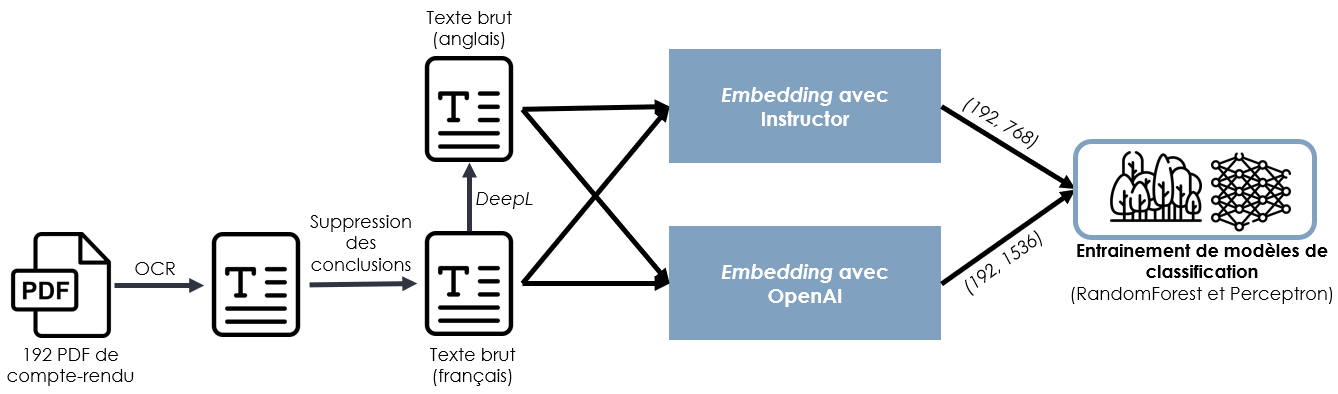
\includegraphics[width=1\textwidth]{figures/myoclassify_flow.png}
 \caption[Entraînement modèle \textit{MyoClassify}]{\textbf{Étapes de préparation et d'entraînement des modèles de \textit{MyoClassify}}}
 \label{fig:myoclassify_flow}
\end{figure}
\subsection{Méthodologie}
La figure \ref{fig:myoclassify_flow} représente l'ensemble des étapes réalisées pour préparer les données et entraîner un modèle de classification. Pour l'ensemble de ces rapports, nous avons réalisé une étape de détection de texte par \gls{ocr} avec \textit{Tesseract} (présenté dans le chapitre 4 "Matériels et méthodes" ainsi que dans le chapitre 5 sur \gls{impatient}). Ensuite, nous avons retiré les conclusions des rapports (indiquant la décision de diagnostic final, c'est-à-dire le label), afin que le modèle n'ait pas accès au diagnostic réel pour prédire le diagnostic. Enfin, à partir de ces conclusions, nous avons labellisé à la main chaque rapport avec un diagnostic parmi les 5 catégories listées ci-dessus.

Le contenu de chaque rapport (texte brut sans la partie conclusion) a été traduit en anglais grâce à l'\gls{api} DeepL afin de comparer les performances sur les textes anglais (traduit) et français (orignaux). Puis ces textes ont été encodés numériquement grâce à deux modèles\gls{llms} d'\textit{embedding} (présenter dans le chapitre 4 "Matériel et méthodes"): le modèle d'OpenAI (disponible uniquement \textit{via} \gls{api}) et le modèle \textit{Instructor-Large} (autohébergé). Les modèles d'\textit{embedding} sont des modèles qui prennent en entrée un texte (un mot, une phrase, un paragraphe ou un document) et qui produisent en sortie un vecteur numérique de grande taille capturant le sens sémantique du document d'entrée. Le modèle d'\textit{embedding} commercial d'OpenAI qui transforme les documents en vecteur de taille (1, 1536), tandis que le modèle auto hébergée libre et open source nommé \textit{Instructor-Large} qui transforme les documents en vecteur de taille (1, 768). Ces modèles sont des boites noires, c'est-à-dire que la signification des centaines (voire des milliers dans le cas d'OpenAI) de valeurs numériques décrivant le document n’est pas connue, cependant elles représentent le sens sémantique du texte.
À partir de ces 4 jeux de données (192 rapports dans 4 conditions: français/anglais et \textit{embedding} par OpenAI/Instructor), nous avons entrainé et comparé les performances pour la prédiction de diagnostic de deux algorithmes: les \textit{random forest} et les perceptrons (réseaux de neurones simples). Nous avons retiré du jeu de données les 54 rapports sans diagnostic, car ils ne peuvent pas être utilisés pour l'entraînement des modèles à apprentissage supervisé, ce qui aboutit à 138 rapports utilisés sur 4 labels différents pour l'entraînement des modèles (\gls{nm}, \gls{com}, \gls{cnm}, non-CM).
\begin{table}[!ht]
\centering
\caption[Nombre de comptes rendus de biopsies par diagnostic]{\textbf{Nombre de comptes rendus de biopsies par diagnostic}. Au total, ce sont 192 comptes rendus de biopsies répartis sur 5 labels différents, dont les 3 grands sous-types de myopathies congénitales (NM, COM, CNM), un label pour les comptes rendus sans diagnostics (UNCLEAR) et un label pour les comptes rendus non liés aux myopathies congénitales.}
\label{tab:number_patients}
\begin{tabular}{|l|c|}
\hline
\textbf{Diagnostic} & \textbf{Nombre de rapports} \\
\hline
Myopathie à Némaline (NM) & 44 \\
\hline
Myopathie à Cores (COM) & 48 \\
\hline
Myopathie centronucléaire (CNM) & 16 \\
\hline
Diagnostic non établi (UNCLEAR) & 54 \\
\hline
Autre (non-CM) & 30 \\
\hline
\end{tabular}
\end{table}

\subsection{Résultats des entraînements et performances des systèmes d'\textit{embedding}}
Au total, 8 conditions expérimentales pour la prédiction de diagnostics ont été évaluées: \textit{Embedding} OpenAI vs Instructor, rapports en Français vs traduits Anglais, \textit{Random Forest} vs Perceptrons (représenté en figure \ref{fig:myoclassify_flow}). Pour chacune des conditions expérimentales, les hyperparamètres des modèles ont été optimisés par grille et les performances ont été évaluées grâce à 10 cross-validations. Ceci a été fait pour (i) obtenir des modèles avec les meilleures performances possibles (optimisation par grille) et (ii) avoir une estimation robuste des performances (moyenne sur 10 essais par cross-validation). L'ensemble des résultats de ces entraînements (métriques de performances et modèles) sont disponibles en ligne à l'adresse: \url{https://wandb.ai/lambda-science/myo-text-classify/reports/MyoClassify-all-conditions-results--Vmlldzo0NDMyMTcw}.
\begin{table}[!ht]
\centering
\caption[Récapitulatif des performances des modèles \textit{MyoClassify}]{\textbf{Récapitulatif des performances des modèles \textit{MyoClassify}}. Pour chaque modèle, les valeurs d'exactitude, d'exactitude équilibrée, de score F1 pondéré et macro et de score F1 uniquement pour le classe CNM ont été mesurées.}
\label{tab:myoclassify_metrics}
\begin{tabularx}{\textwidth}{|X|c|c|c|c|c|}
\hline
\textbf{Nom} & \textbf{Exactitude} & \textbf{Exact. Equi.} & \textbf{F1 pond.} & \textbf{F1-Macro} & \textbf{F1 CNM} \\\hline
Instructor FR RF & 0.65 & 0.56 & 0.62 & 0.54 & 0.11 \\ \hline
Instructor EN RF & 0.67 & 0.54 & 0.62 & 0.52 & 0.00 \\ \hline
Instructor FR MLPC & 0.67 & 0.57 & 0.66 & 0.56 & 0.08 \\ \hline
Instructor EN MLPC & 0.64 & 0.58 & 0.64 & 0.58 & 0.32 \\ \hline
Openai FR RF & 0.61 & 0.56 & 0.60 & 0.58 & 0.45 \\ \hline
Openai EN RF & 0.65 & 0.5792 & 0.64 & 0.60 & 0.40 \\ \hline
Openai FR MLPC & 0.64 & 0.6 & 0.64 & 0.61 & 0.54 \\ \hline
\textbf{Openai EN MLPC} & \textbf{0.70} &\textbf{0.67}& \textbf{0.69} &\textbf{ 0.68} & \textbf{0.64} \\ \hline
\end{tabularx}
\end{table}
\begin{figure}[!ht]
 \centering
 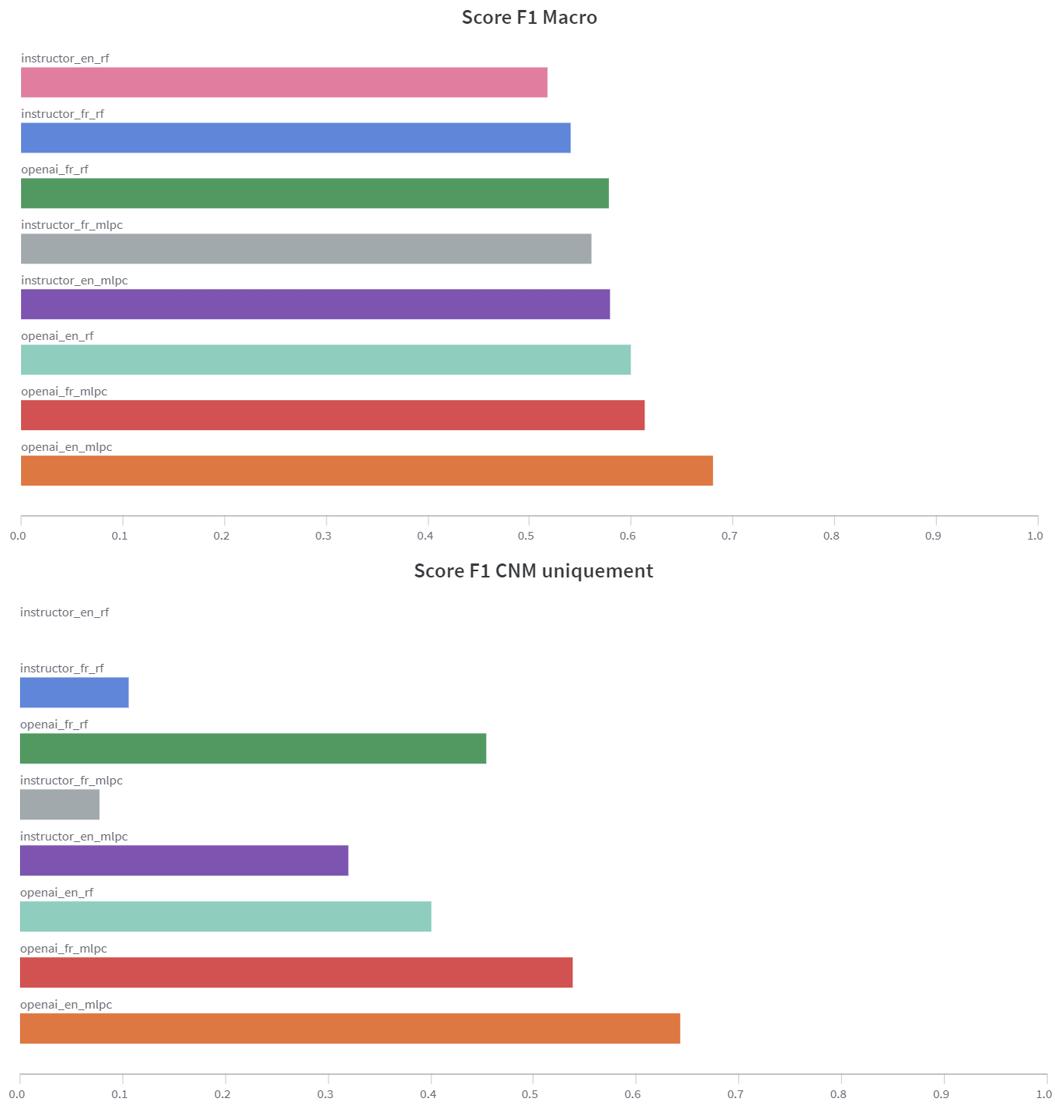
\includegraphics[width=1\textwidth]{figures/histo_myoclassify.png}
 \caption[Histogrammes des performances des modèle MyoClassify]{\textbf{Histogrammes des performances des modèles \textit{MyoClassify}} pour le score F1-macro (haut) et le score F1 pour la classe minoritaire (CNM) uniquement (bas). Globalement, le modèle le plus performant est le modèle \textit{OpenAI\_EN\_MLPC} pour les deux métriques présentées.}
 \label{fig:myoclassify_histo}
\end{figure}
\begin{figure}[!ht]
 \centering
 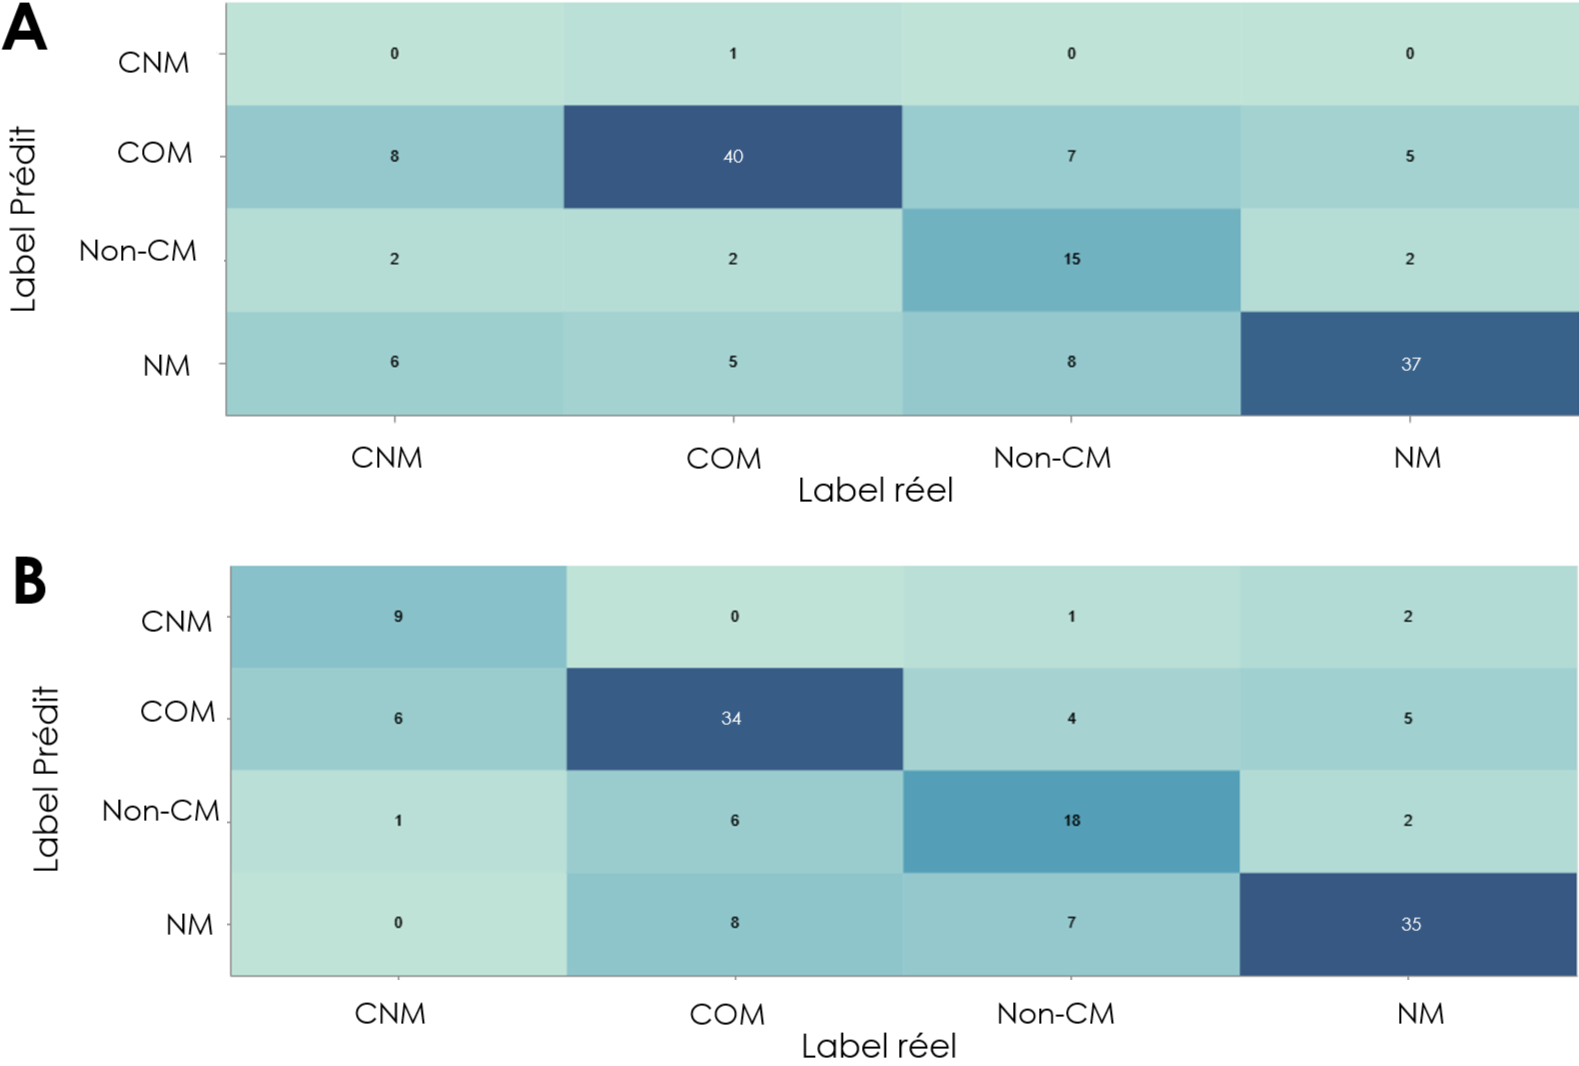
\includegraphics[width=1\textwidth]{figures/matrix_conf_myoclassify.png}
 \caption[Matrice de confusion \textit{MyoClassify}]{\textbf{Matrice de confusion des modèles} \textit{\textbf{MyoClassify}} pour le moins bon (\textit{instructor\_en\_rf} en haut) et le meilleur modèle (\textit{openai\_en\_mlpc} en bas) en termes de score F1.}
 \label{fig:myoclassify_conf}
\end{figure}

Sur le tableau \ref{tab:myoclassify_metrics} et les figures \ref{fig:myoclassify_histo} et \ref{fig:myoclassify_conf} on observe que, globalement, les performances à travers les conditions en termes de score F1 sont situées dans un intervalle entre 0.51 et 0.68 et que donc toutes les méthodes ont réalisé des erreurs de prédiction. Les modèles entraînés sur la base du modèle d'\textit{embedding} autohébergé \textit{Instructor} ont de moins bonnes performances globales à travers toutes les conditions. Cependant si l'on observe la matrice de confusion (\ref{fig:myoclassify_conf}), on observe que le moins bon modèle \textit{Instructor} a obtenu de meilleures performances de classifications que le meilleur modèle \textit{OpenAI} pour les deux classes de myopathies majoritaires: \gls{nm} et \gls{com} (40 prédictions correctes contre 34 pour les \gls{nm}, et 37 prédictions correctes contre 35 pour les \gls{com}). Cela indique donc que les métriques de performances globales sont donc très influencées par les performances du modèle sur les \gls{cnm}.

Pour la classe minoritaire (les \gls{cnm} avec 16 rapports), les performances des modèles sont très faibles pour l'\textit{embedding} du modèle \textit{Instructor}. Par exemple, pour notre modèle \textit{Instructor\_FR\_RF}, aucune \gls{cnm} n'a été prédite (matrice de confusion \ref{fig:myoclassify_conf}). Le modèle \textit{OpenAI\_EN\_MLPC} quant à lui obtient de meilleures performances et a été capable de prédire 9 des 16 \gls{cnm}. 

Dans le cadre du modèle d'\textit{embedding} d'OpenAI, la traduction des rapports en anglais a permis d'obtenir de meilleures performances dans toutes les conditions. De même, l'utilisation d'un perceptron multicouche a permis d'obtenir de meilleures performances en termes de score F1 dans toutes les conditions par rapport à la \textit{random forest}.

En termes de performances brutes, il semble recommandable de: (i) traduire les comptes rendus en anglais (ii) d'utiliser le modèle d'OpenAI pour l'\textit{embedding} et (iii) d'entrainer un perceptron multicouche pour apprendre à différencier les diagnostics en fonction de la représentation numérique des rapports (\textit{embeddings}).

\section{\textit{MyoSearch}: un moteur de recherche de patients}
En utilisant les techniques d'\textit{embedding}  pour représenter un texte sous forme numérique en capturant son sens sémantique, il est alors possible de calculer un score de similarité entre une requête en texte libre et une masse de documents pour trouver le document le plus proche. Avec \textit{MyoSearch} nous avons créé un outil qui permet de faire des requêtes en texte libre parmi l'ensemble des rapports de biopsies de patients. Il est alors possible de chercher rapidement chez quels patients un symptôme ou diagnostic particulier est présent. Cette création de moteur de recherche est totalement automatique et ne nécessite aucun travail d'annotation, contrairement à l'annotation de comptes rendus dans \gls{impatient}. Elle se déroule en deux phases: (i) l'intégration des données pour constituer la base de données puis (ii) la phase de requêtage de la base de données en fonction de l'entrée de l'utilisateur.

\subsection{Intégration des rapports: création de la base de données de vecteurs}
\begin{figure}[!ht]
 \centering
 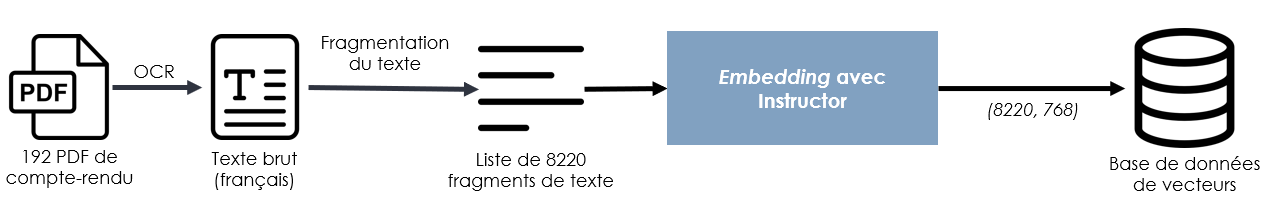
\includegraphics[width=1\textwidth]{figures/myosearch_ingest.png}
 \caption[Intégration des données dans \textit{MyoSearch}]{\textbf{Schéma de l'intégration des données pour le moteur de recherche \textit{MyoSearch}}. L'ensemble des comptes rendus de biopsie sont fragmentés et chaque fragment est transformé en vecteur numérique par le modèle d'\textit{embedding}. Chacune de ces représentations est intégrée dans la base de données de vecteurs.}
 \label{fig:myosearch_ingest}
\end{figure}

À la différence de \textit{MyoClassify}, cette fois-ci nous ne voulons pas générer 1 \textit{embedding} par document, mais plutôt séparer les documents en fragments et avoir un \textit{embedding} par fragment de document. Nous avons choisi de découper les documents en fragments de la taille d'une phrase et ainsi d'obtenir un \textit{embedding} pour chaque phrase du document. Ceci permet d'obtenir de meilleur résultat lors du requêtage de la base de données, car le sens sémantique de chaque phrase va pouvoir être comparé à la requête, plutôt que la moyenne de l'ensemble du document.

La figure \ref{fig:myosearch_ingest} présente la phase d'intégration des données. Nous avons d'abord détecté le texte des rapports PDF par \gls{ocr}. Comme cette détection est hétérogène et bruitée (images de texte dégradées, difficulté de reconnaissance des caractères), il est difficile de trouver les bornes exactes des phrases. Dès lors, nous avons à fragmenter le contenu en morceaux de taille maximale de 100 \textit{tokens} (environ 15 à 30 mots français) avec un recouvrement de 50, soit la taille moyenne d'une phrase en français. Pour 192 rapports, cela représente 8220 fragments de texte. Pour ces 8220 fragments, nous avons calculé leur représentation numérique (\textit{embedding}) et les avons intégrés dans une base de données de vecteurs. Enfin pour chaque fragment, il est possible d'ajouter des métadonnées qui peuvent servir de filtre pour les requêtes comme le diagnostic final ou le gène responsable de la maladie.

\subsection{Requêtage des données}
\begin{figure}[!ht]
 \centering
 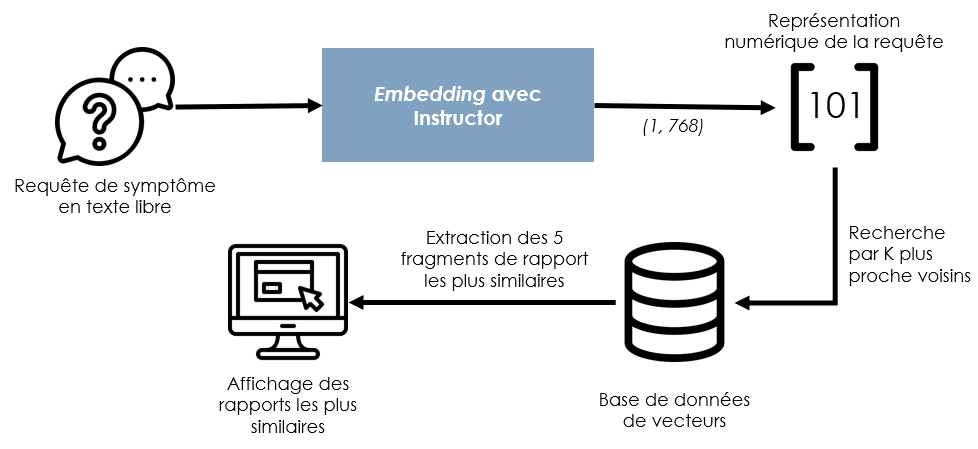
\includegraphics[width=1\textwidth]{figures/myosearch_query.png}
 \caption[Requêtage des données dans \textit{MyoSearch}]{\textbf{Schéma du requêtage des données dans \textit{MyoSearch}}. La requête formulée par l'utilisation est convertie en vecteur numérique qui est ensuite comparé (par similarité) à l'ensemble des fragments de comptes rendus intégré dans la base de données de vecteur.}
 \label{fig:myosearch_query}
\end{figure}
Quand l'ensemble des documents a été découpé et intégré dans la base de données, il est possible de réaliser des requêtes. La figure \ref{fig:myosearch_query} présente la phase de requêtage des données. L'utilisateur peut fournir \textit{via} l'interface web un symptôme d'intérêt en texte libre tel que "surcharge lipidique". Cette requête va ensuite être transformée en vecteur numérique par le modèle d'\textit{embedding }\textit{Instructor}. Ce vecteur va être comparé à la base de données de vecteurs pour rechercher les tops 5 plus proches voisins grâce à un algorithme nommé \textit{Hierarchical Navigable Small Worlds, HNSW}. Les cinq fragments avec les scores de similarité les plus élevés sont ensuite affichés sur l'interface web. Le tableau \ref{tab:myosearch_results} présente les résultats obtenus pour une requête dans MyoSearch. Par exemple pour la requête "surcharge lipidique" les trois rapports les plus proches font mention d'une surcharge en lipides chez des patients dont (i) le diagnostic n'est pas connu (ii) le diagnostic n'est pas une myopathie congénitale et (iii) chez un patient avec une \gls{nm}. Cette recherche est aussi multilingue, le modèle d'\textit{embedding} autorise des recherches entre une base de données française avec requête en anglais, ou inversement.
\begin{table}[!ht]
\centering
\caption[Exemple d'une requête et des résultats de \textit{MyoSearch}]{\textbf{Exemple d'une requête et des résultats de \textit{MyoSearch}}}
\label{tab:myosearch_results}
\begin{tabularx}{\textwidth}{|l|X|p{1cm}|p{2cm}|}
\hline
\textbf{Requête} & \textbf{Fragment le plus similaire} & \textbf{Rang} & \textbf{Rapport et diagnostic} \\\hline
"surcharge lipidique" & "d’inclusions. Il est à noter que l’on observe également une surcharge importante en lipides dans" \newline & 1 & 13405-105.txt UNCLEAR \\
 & "une myopathie congénitale. D'autre part, une surcharge importante en lipides qui nécessite"\newline & 2 & 11391-79.txt non-CM \\
 & "de surcharge en lipides - Technique de Koëlle : CONCLUSIONS : Anomalies caractéristiques d’une" & 3 & 5060-35.txt NM \\ \hline
\end{tabularx}
\end{table}

\section{Déploiement de l'outil}
Développé de façon \textit{open-source}, le code source de \gls{nlmyo} est disponible sur GitHub à l'adresse: \url{https://github.com/lambda-science/NLMyo} sous une licence AGPL-3 assurant le statut open source de l'outil. Une version de démonstration en ligne est déployée grâce à \textit{Streamlit} à l'adresse \url{https://lbgi.fr/NLMyo/}. Comme \gls{nlmyo} propose l'utilisation de \gls{llms} autohébergé, l'outil est hébergé sur un serveur avec un processeur 64 cœurs pour accélérer l'inférence du notre \gls{llms}. Si l'outil n'utilise que l'API OpenAI comme modèle génératif et d'\textit{embedding} alors il est possible d'héberger l'application sur un serveur nécessitant ainsi très peu de ressource de calcul.

\section{Discussions et perspectives de développement}
\gls{nlmyo} met à disposition des outils permettant le traitement de façon massive de rapports de comptes rendus médicaux et notamment des rapports de biopsie. Cependant, les défis pour rendre l'outil plus robuste sont multiples. 

Le premier défi concerne MyoSearch, le moteur de recherche de données de patients. Bien que la méthode soit fonctionnelle et novatrice, les résultats obtenus ne sont pas tout le temps similaire à la requête. Un travail d'amélioration des méthodes de fragmentation et de requêtage est nécessaire. De plus, il n'est actuellement possible que de chercher un symptôme à la fois, il faudrait créer un système permettant de croiser les résultats des requêtes pour plusieurs symptômes, permettant ainsi de chercher un profil de symptômes complet. De plus, l'ajout de métadonnées supplémentaires aux fragments (informations plus complètes sur le patient telles que le gène muté, l'âge, le muscle de la biopsie) sur les patients permettrait de réaliser des requêtes plus fines pour ne sélectionner, par exemple, que les patients liés à un gène en particulier.

Le second défi majeur concerne la protection de la confidentialité des données de santé. En effet, certains outils, pour obtenir les meilleures performances, reposent sur l'utilisation de \gls{llms} externes \textit{via} des l'\gls{api} OpenAI, ce qui est problématique dans le cadre de données sensibles, même anonymisées. Pour cela, nous avons aussi proposé une alternative avec un modèle autohébergé, mais pour l'instant celui-ci sous-performe. Par exemple dans \textit{MyoExtract}, les informations extraites sont incomplètes et dans \textit{MyoClassify} les scores d'exactitude et F1 sont globalement plus faibles, voire très faibles, pour la classe minoritaire (\gls{cnm}). Cependant, la recherche en terme de \gls{llms} est un domaine très dynamique et il est très probable qu'une solution autohébergée et performante soit disponible sous peu.
\chapter{Vers une génération de rapports automatiques à partir d’imagerie avec MyoQuant}
\section{Contexte}
Les outils présentés précédemment ont pour vocation de traiter et d'explorer les comptes-rendus de biopsies textuels, permettant ainsi une approche rétrospective de l'ensemble des patients connus à ce jour. Cependant, il est intéressant d'explorer aussi comment l'analyse d'images par \gls{ia} peut permettre de générer automatiquement des comptes-rendus de biopsies. Cette approche permettrait un grain de précision et de temps dans l'évaluation des biopsies. Tout d'abord un gain de temps, car une approche par \gls{ia} permettrait de traiter  plusieurs biopsies de grande taille de manière automatique, libérant ainsi le temps utilisé pour l'évaluation des coupes histologiques. Ensuite un gain de précision, car l'évaluation des biopsies par un expert humain est en général qualitative. La description de phénotype se limite généralement à des adjectifs de quantité tels que "peu", "moyen" ou "beaucoup". Grâce à une approche de comptage par \gls{ia}, il est alors possible d'obtenir la quantité précise de fibres présentant un noyau centralisé par exemple et ainsi de pouvoir établir des seuils pour une analyse plus approfondie.

\gls{myoquant}, l'outil présenté dans ce chapitre, est une suite de méthodes pour quantifier différents marqueurs pathologiques dans les biopsies de \gls{mc}. \gls{myoquant} intègre soit des méthodes algorithmiques simples basées sur des modèles d'\gls{ia} généralistes en histologie comme CellPose (\cite{stringer_cellpose_2021}) et Stardist (\cite{weigert_star-convex_2020}), soit des méthodes basées sur des modèles \gls{ia} développés à partir de nos données. Actuellement, \gls{myoquant} est capable de quantifier des marqueurs pathologiques dans trois des cinq colorations réalisées en routine lors du diagnostic des \gls{mc}: la centralisation des noyaux à la coloration \gls{he}, un déséquilibre dans le ratio des fibres de type 1 et 2 à la coloration ATPase et une répartition anormale des mitochondries dans les fibres musculaires à la coloration \gls{sdh}. Dans ce chapitre, nous allons voir comment ont été implémentées ces solutions de quantification automatique et des exemples d'application.

\begin{figure}[!ht]
 \centering
 
\includegraphics[width=0.66\textwidth]{figures/myoquant_logo.png}
 \caption[Logo MyoQuant]{Logo de MyoQuant}
 \label{fig:myoquant_logo}
\end{figure}

\section{Analyse de la position des noyaux cellulaires}
Dans un premier temps, nous nous sommes intéressés à l'analyse de la position des noyaux cellulaires dans les fibres musculaires. Dans un muscle sain, les noyaux sont en général en périphérie des fibres, tandis que dans les muscles des patients atteints de \gls{mc} et particulièrement dans les \gls{cnm}, les noyaux peuvent être internalisés voire centralisés. Par exemple, dans la figure \ref{fig:he_example}, on observe un nombre important de fibres ayant un noyau cellulaire internalisé. Nous avons dès lors développé une méthode pour compter automatiquement le nombre de fibres présentant un noyau internalisé.
\begin{figure}[!ht]
 \centering
 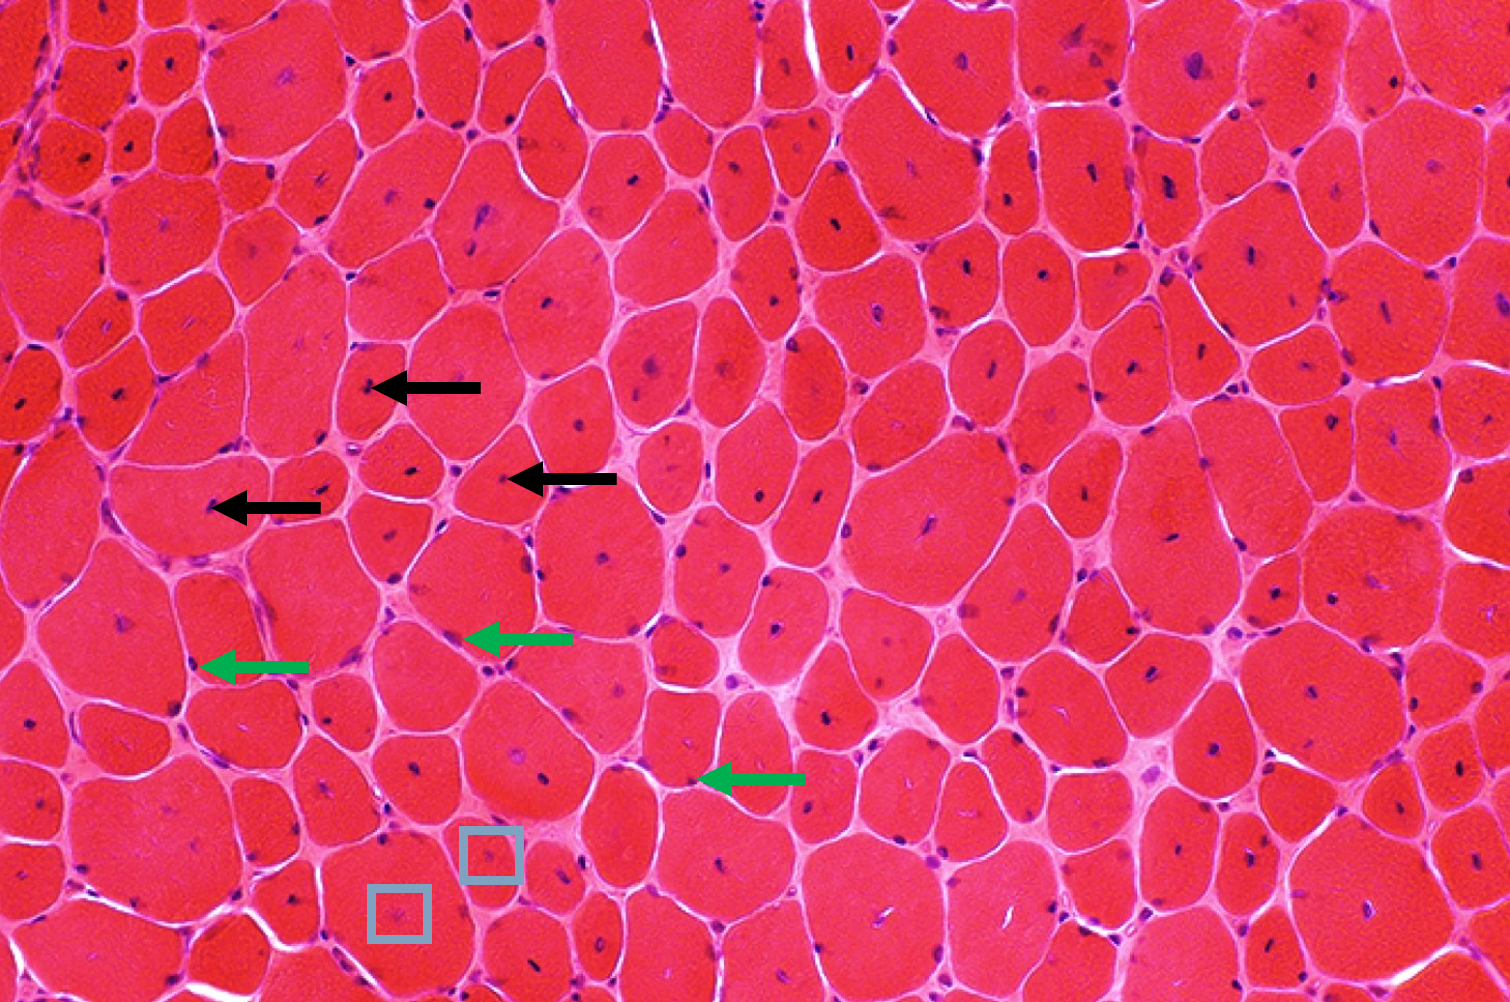
\includegraphics[width=0.8\textwidth]{figures/he_example.jpg}
 \caption[Exemple de biopsie musculaire à la coloration HE]{Exemple de biopsie musculaire de CNM à la coloration HE dans laquelle on observe des fibres avec des noyaux centralisés.}
 \label{fig:he_example}
\end{figure}

\subsection{Algorithme de quantification}
Pour réaliser cette quantification, la première étape consiste à segmenter, c'est-à-dire à obtenir la position de toutes les fibres musculaires et de tous les noyaux de la coupe. Pour cela nous avons utilisé deux modèles d'\gls{ia} généralistes développés spécifiques pour l'analyse de coupes histologiques: Cellpose et Stardist. Cellpose nous a permis de segmenter les fibres musculaires, tandis que Stardist nous a permis de segmenter les noyaux cellulaires. La figure \ref{fig:he_seg} présente les résultats de la segmentation de la biopsie présentée en figure \ref{fig:he_example}. On observe que globalement toutes les fibres musculaires sont bien segmentées, cependant concernant les noyaux cellulaires, certains sont trop peu colorés pour être reconnus par le modèle. C'est notamment le cas pour quelques noyaux centraux sur la gauche de la biopsie. Ce qui sera problématique lors de l'analyse des noyaux, car ils ne seront pas considérés.
\begin{figure}[!ht]
 \centering
 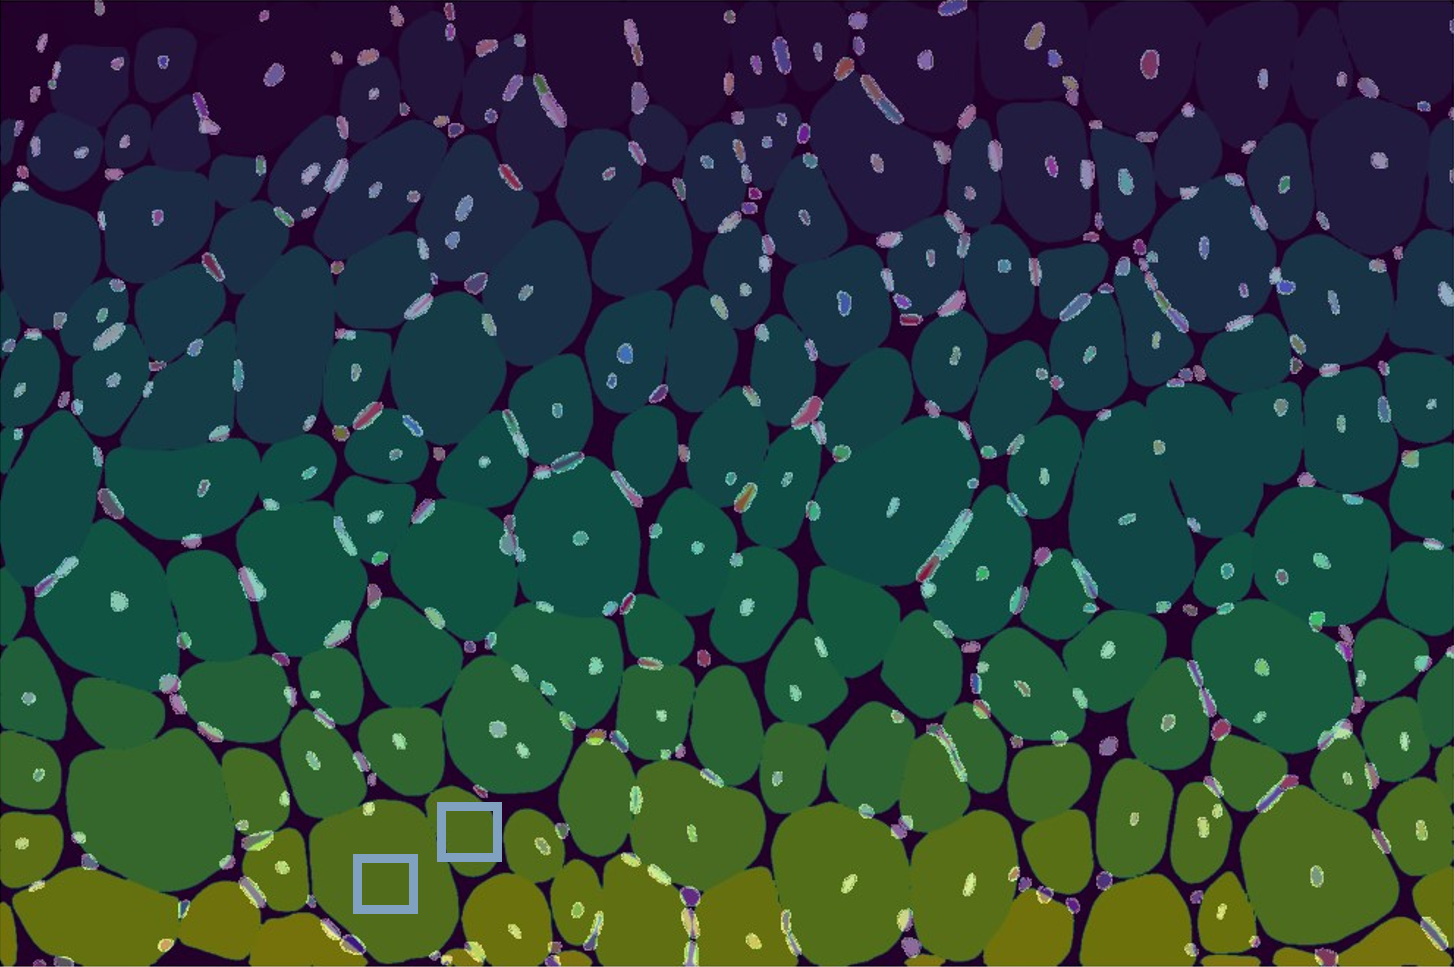
\includegraphics[width=0.8\textwidth]{figures/he_seg.png}
 \caption[Exemple de segmentation de biopsie par Cellpose et Stardist]{Exemple de segmentation des fibres musculaires et des noyaux cellulaires par Cellpose et Stardist}
 \label{fig:he_seg}
\end{figure}

Après avoir obtenu la position de chaque fibre et noyau, nous évaluons la position de chaque noyau, fibre par fibre. Cette évaluation repose sur le calcul de ce que l'on appelle un score d'excentricité. Ce score est calculé selon la formule suivante:

\(\text{Score d'excentricité} = \frac{\text{Dist. centre fibre et noyau}}{\text{Dist. centre fibre et membrane}}\)

Dans cette formule, la notation "Dist. centre fibre et noyau" représente la distance en pixels entre le centroïde de la fibre musculaire et centroïde du noyau considéré. Et la notation "Dist. centre fibre et membrane" représente la distance entre le centroïde de la fibre musculaire et la membrane cellulaire selon une droite passant par le noyau d'intérêt. La figure \ref{fig:he_single_nuc}  présente la classification des noyaux d'une fibre musculaire unique. Quatre noyaux ont été détectés dans cette fibre dont trois ont un score d'excentricité supérieur à 0,9 et un inférieur à 0,1. En fixant un seuil de façon empirique à 0,75, on considère alors que cette fibre musculaire possède un noyau internalisé.
\begin{figure}[!ht]
 \centering
 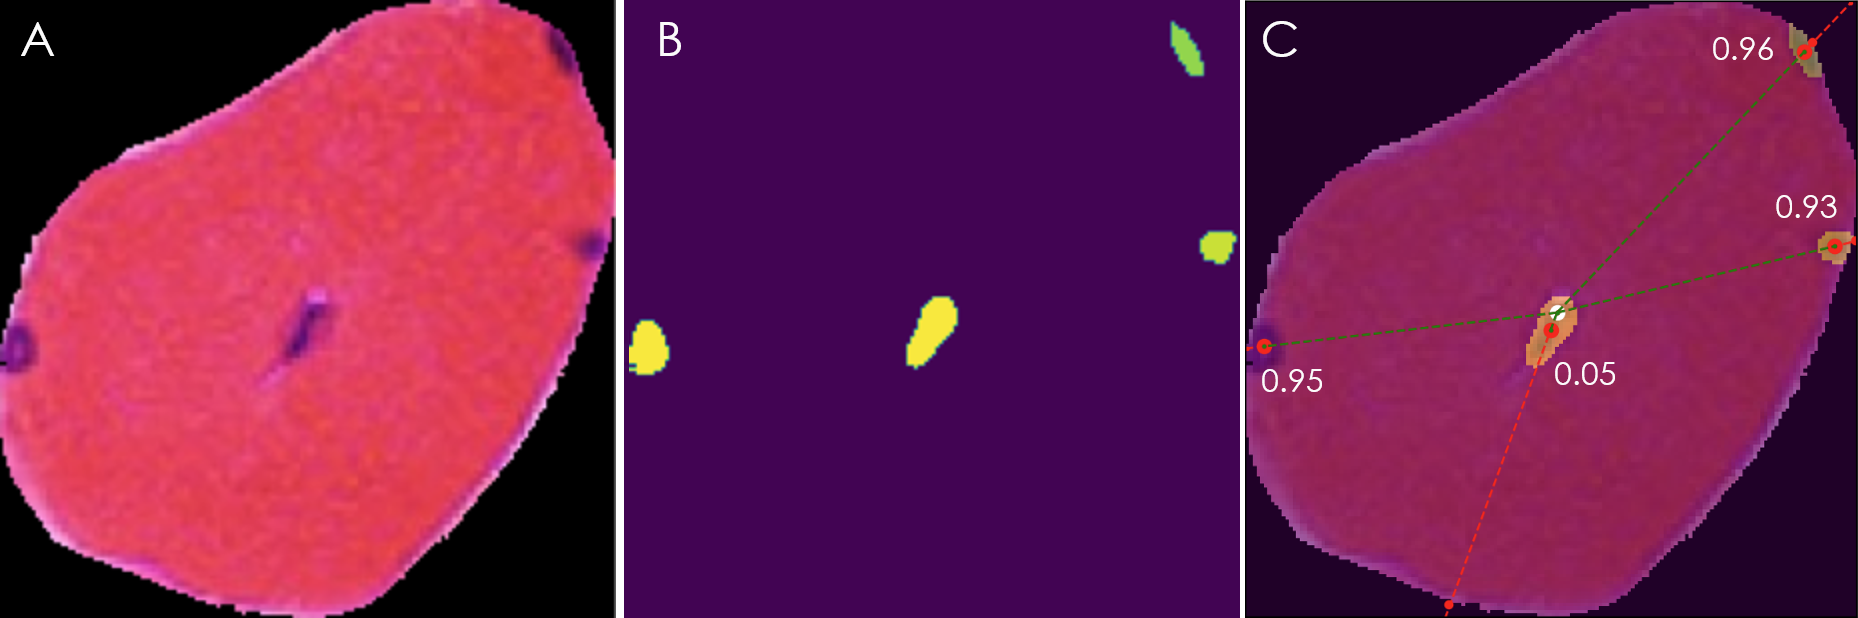
\includegraphics[width=1\textwidth]{figures/he_single_nuc.png}
 \caption[Exemple de classification de la position des noyaux]{Exemple de classification de la position des noyaux cellulaires d'une fibre musculaire. \textbf{(A)} La fibre musculaire seule,\textbf{ (B)} masque de segmentation des 4 noyaux pour cette fibre,\textbf{ (C)} schéma de la classification des noyaux avec le score d'excentricité de chaque noyau représentant le ratio de distance: centre de la fibre - noyau versus centre de la fibre - membrane cellulaire.}
 \label{fig:he_single_nuc}
\end{figure}
En comparant l'ensemble des noyaux de chaque fibre à un seuil (ici fixé à 0,75), on peut alors quantifier le nombre de fibres musculaires ayant au moins un ou plusieurs noyaux internalisés. Par exemple, pour l'image présentée en figure \ref{fig:he_example}, la figure \ref{fig:he_paint} présente les résultats de cette classification. Sur cette coupe histologique, on obtient un total de 74 fibres (soit 42\% des fibres) avec au moins un noyau internalisé.
\begin{figure}[!ht]
 \centering
 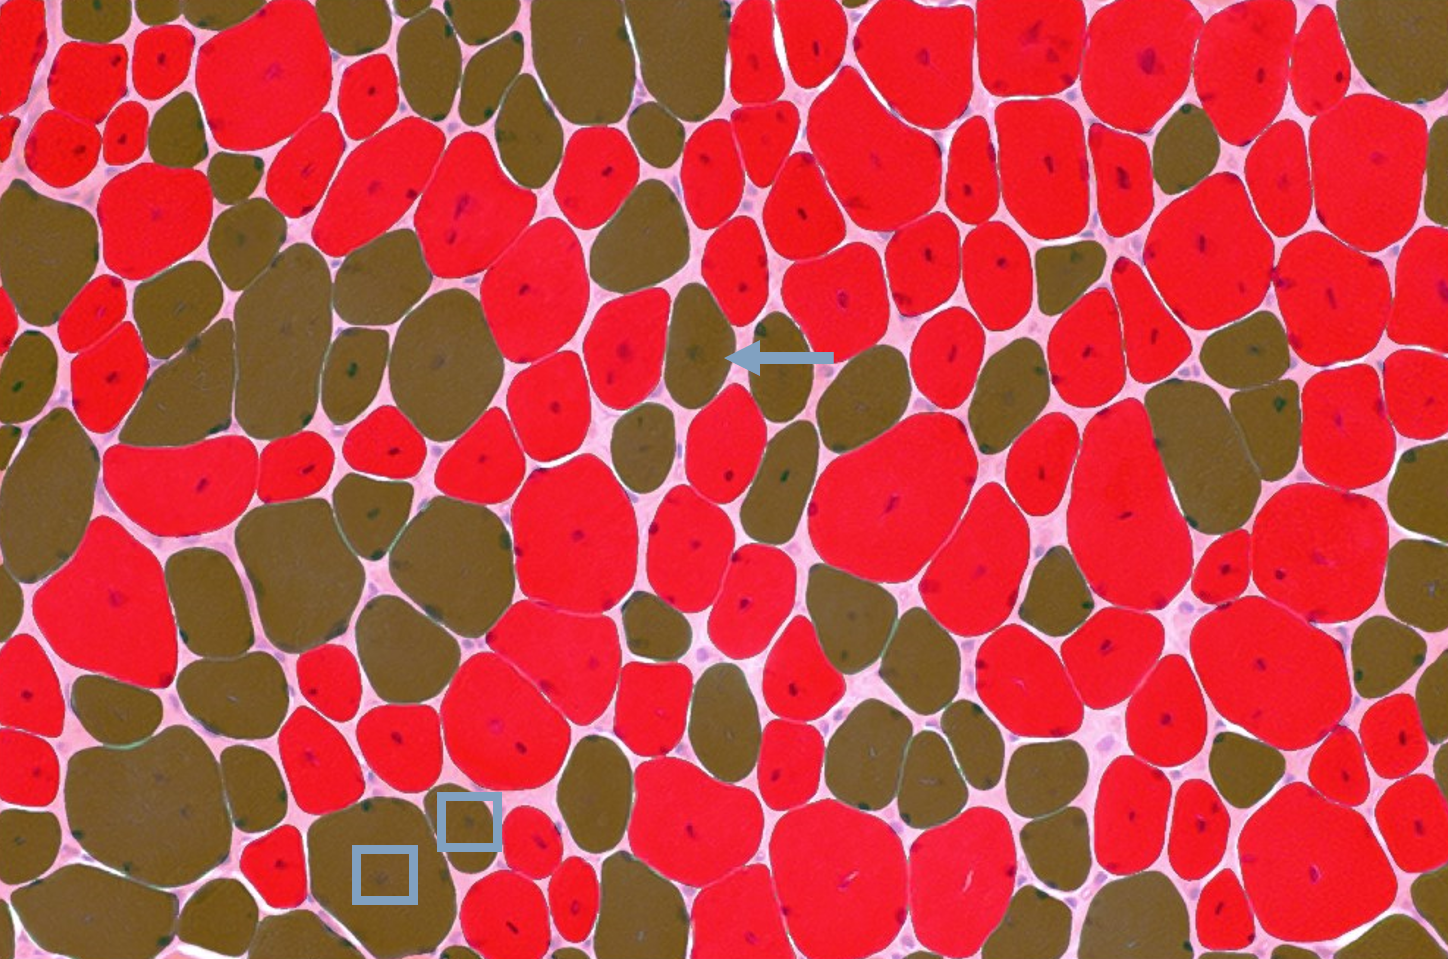
\includegraphics[width=0.8\textwidth]{figures/he_paint.png}
 \caption[Exemple de classification de biopsie musculaire à la coloration HE]{Exemple de classification de biopsie musculaire à la coloration HE. Colorées en vert les fibres sans noyau internalisé, et en rouge les fibres avec au moins un noyau internalisé (score d'excentricité inférieur à 0.75)}
 \label{fig:he_paint}
\end{figure}

\subsection{Exemple d'application: quantification de la régénération musculaire }
La présence de noyaux centralisés dans les fibres musculaires est un marqueur pathologique dans les biopsies de \gls{mc}. Cependant, cette centralisation peut aussi être synonyme de régénération musculaire chez les individus sains. Ainsi, la quantification du nombre de noyaux centralisés est donc aussi un moyen de quantifier la régénération musculaire dans une coupe histologique. Dans le cadre d'une collaboration avec l'\gls{igbmc} et plus spécifiquement, avec l'équipe Biologie moléculaire et cellulaire des cancers du sein du Dr. Tomasetto, nous avons utilisé \gls{myoquant} pour évaluer la quantité de régénération musculaire chez des souris traitées avec une drogue induisant le processus régénératif. Ces images d'histologie sont des images à fluorescence (et non à la coloration \gls{he}) avec un fluorochrome pour la membrane cellulaire et un fluorochrome pour les noyaux cellulaires. L'algorithme de \gls{myoquant} est directement compatible avec les images à fluorescence et fonctionne de la même façon que pour les images à coloration\gls{he}
\begin{figure}[!ht]
 \centering
 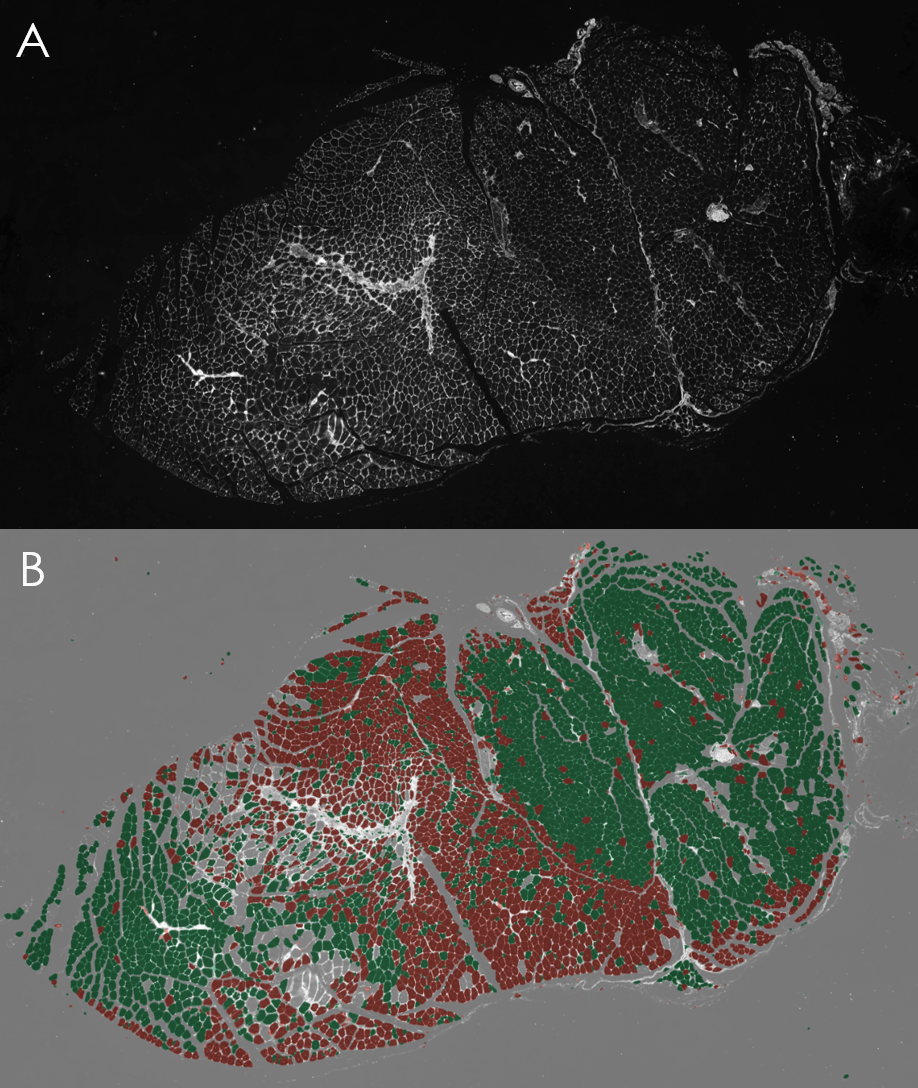
\includegraphics[width=0.8\textwidth]{figures/fluo_nuc.png}
 \caption[Exemple de classification de biopsie musculaire pour la régénération musculaire]{Exemple de classification de biopsie musculaire pour la régénération musculaire. Colorées en vert les fibres sans noyau internalisé (fibres normales), en rouge les fibres avec au moins un noyau internalisé (en régénération)}
 \label{fig:fluo_paint}
\end{figure}

La figure \ref{fig:fluo_paint} présente un exemple de coupe complète de biopsie musculaire de souris avec le masque de quantification associé généré par \gls{myoquant}. Sur cette image, il y a 6078 fibres musculaires détectées, dont 2285 (environ 35\%) sont en régénération. Le tableau \ref{tab:myoquant_fluo_time} présente le temps de calcul nécessaire pour chaque étape de la quantification pour la coupe \ref{fig:fluo_paint} et le tableau \ref{tab:myoquant_fluo_results} présente les résultats de cette quantification. On observe que pour traiter une coupe complète sur une machine sans matériel spécifique (sans \gls{gpu}) il a nécessité environ 1 heure de calcul, dont la majorité a été utilisée par le programme Cellpose pour segmenter les fibres musculaires. Cependant, cette vitesse peut être largement améliorée d'un facteur 5 par l'utilisation de matériel spécifique aux calculs \gls{ia} (\gls{gpu}), passant de 3782 secondes pour Cellpose à 652. Ainsi, pour une image contenant 6078 fibres et 23 628 noyaux, cela représente environ 1.6 fibre traitée par seconde. Cette quantification a mis en évidence que 37\% des fibres présentaient un noyau internalisé et donc sont en régénération.
\begin{table}[!ht]
\centering
\caption{Temps de calcul pour l'analyse des noyaux d'une coupe complète (6078 fibres, 12000 x 9600 pixels)}
\label{tab:myoquant_fluo_time}
\begin{tabularx}{\textwidth}{|l|c|c|X|}
\hline
\textbf{Étape} & \textbf{Temps sur GPU} & \textbf{Temps sur CPU (s)} & \textbf{Fibres par seconde (sur CPU)} \\
\hline
Cellpose & 652 & 3 782 & 1.6 \\
\hline
StarDist & \textit{mémoire insuffisante} & 21 & 29 \\
\hline
Classification des noyaux & 68 & 68 & 89 \\
\hline
\textbf{Total} & \textbf{>720} & \textbf{3 871} & \textbf{1.57} \\
\hline
\end{tabularx}
\end{table}

\begin{table}[!ht]
\centering
\caption{Résultats de la quantification des noyaux d'une coupe complète (6078 fibres, 12000 x 9600 pixels)}
\label{tab:myoquant_fluo_results}
\begin{tabular}{|l|c|c|}
\hline
\textbf{Type} & \textbf{Valeur} & \textbf{Proportion (\%)} \\
\hline
N° Fibres & 6 078 & 100 \\
\hline
N° Fibres avec 1+ noyau internalisé & 2 264 & 37 \\
\hline
\hline
N° Noyaux & 23 628 & 100 \\
\hline
N° Noyaux internalisés & 3 933 & 16 \\
\hline
N° Noyaux périphériques & 17 918 & 76 \\
\hline
N° Noyaux non classés (hors fibres) & 1 777 & 8 \\
\hline
\end{tabular}
\end{table}
Le tableau \ref{fig:fluo_compil} présente l'ensemble des quantifications opérées dans les différentes conditions de traitement et de génotype (au total 35 \gls{wsi} analysées). On observe qu'après traitement avec la \textit{Cardiotoxin}, une drogue induisant la régénération musculaire, une proportion significativement supérieure de fibres ayant un noyau internalisé par rapport aux coupes contrôle. Ces résultats confirment que \gls{myoquant} est bien capable d'évaluer de façon robuste la présence de noyaux internalisés, un marqueur de la régénération musculaire.

\begin{figure}[!ht]
 \centering
 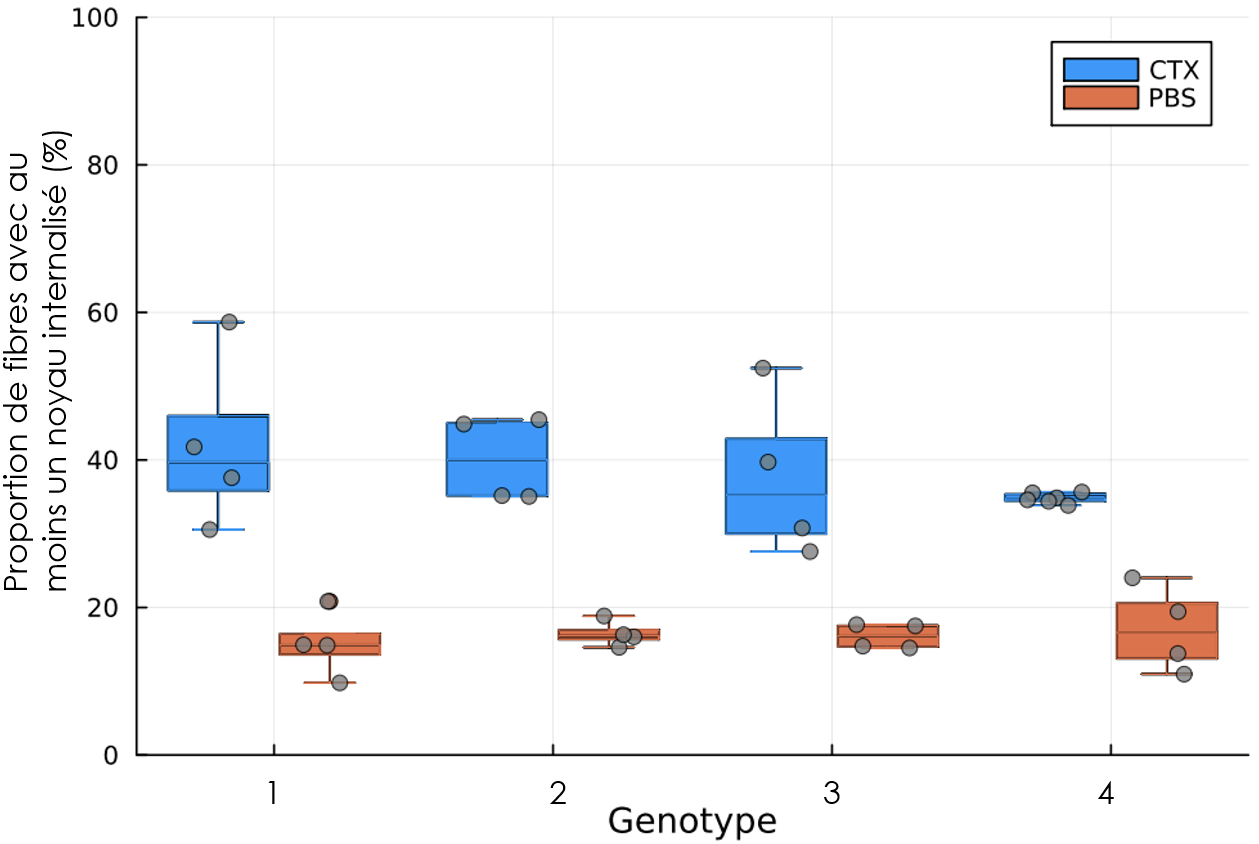
\includegraphics[width=0.8\textwidth]{figures/fluo_compil.png}
 \caption[Résultat de la quantification de la régénération musculaire]{Résultat de la quantification de la régénération musculaire chez des souris pour 4 génotypes différents traités (bleu) ou non (orange) avec une drogue induisant la régénération musculaire}
 \label{fig:fluo_compil}
\end{figure}

\section{Ratio de fibre de type 1 et 2: classification basée sur l'intensité de coloration}

Dans un second temps, nous nous sommes intéressés à l'analyse du ratio des différents types de fibres musculaires dans les biopsies. Dans certaines \gls{mc}, l'équilibre entre fibres de type 1 et type 2 peut être modifié avec une prédominance des fibres de type 1. Les différents types de fibres musculaires sont colorés différentiellement (différence d'intensité) à la coloration ATPase. À un pH 4.3, les fibres de type 1 sont sombres et les fibres de type 2 sont pâles, et inversement au pH 9.4. La figure \ref{fig:atp_example} représente une biopsie musculaire colorée à l'ATPase pH 9.4. On observe assez bien la présence des deux populations de fibres à intensité de coloration distincte et nous avons mis à profit ces différences d'intensité pour développer une méthode de comptage automatique du nombre de fibres de chaque type.
\begin{figure}[!ht]
 \centering
 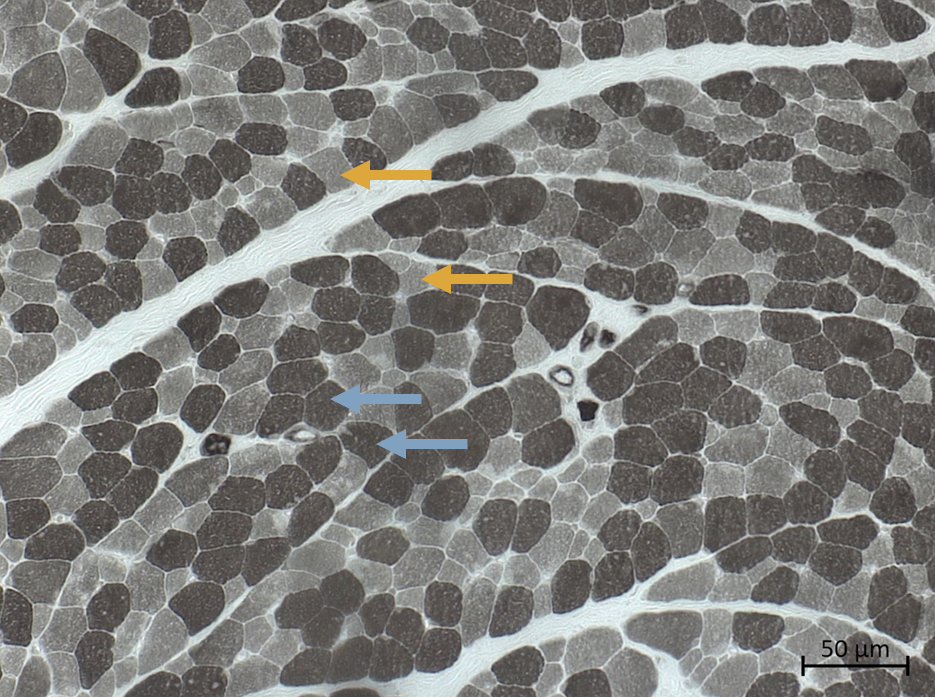
\includegraphics[width=0.8\textwidth]{figures/atp_example.png}
 \caption[Exemple de biopsie musculaire à la coloration ATPase pH 9.4]{Exemple de biopsie musculaire à la coloration ATPase pH 9.4 qui permet de différencier les fibres de type 1 aux fibres de type 2.}
 \label{fig:atp_example}
\end{figure}
\subsection{Algorithme de quantification}
Pour réaliser cette quantification, la première étape consiste à segmenter, c'est-à-dire obtenir la position de toutes les fibres musculaires. Comme précédemment, nous avons utilisé Cellpose afin de segmenter les fibres musculaires. Ensuite, pour chaque fibre, nous avons extrait l'intensité moyenne de la fibre et avons réalisé un histogramme. La figure \ref{fig:atp_density} présente l'histogramme issu de l'analyse de l'image d'exemple pour la coloration ATPase pH 9.4 (\ref{fig:atp_example}). Le but de la procédure est de déterminer automatiquement les pics présents dans l'histogramme et de trouver les minimums locaux entre les pics pour fixer un ou plusieurs seuils d'intensité. Pour cela, à partir des valeurs de cet histogramme, une courbe de densité est créée (par méthode de \gls{kde}). Puis à partir de cette courbe de densité, une méthode de mélange gaussien est utilisée pour déterminer la position des pics dans la courbe de densité. Finalement, le seuil est déterminé en trouvant le minimum local de la courbe de densité entre les deux pics obtenu par mélange gaussien.
\begin{figure}[!ht]
 \centering
 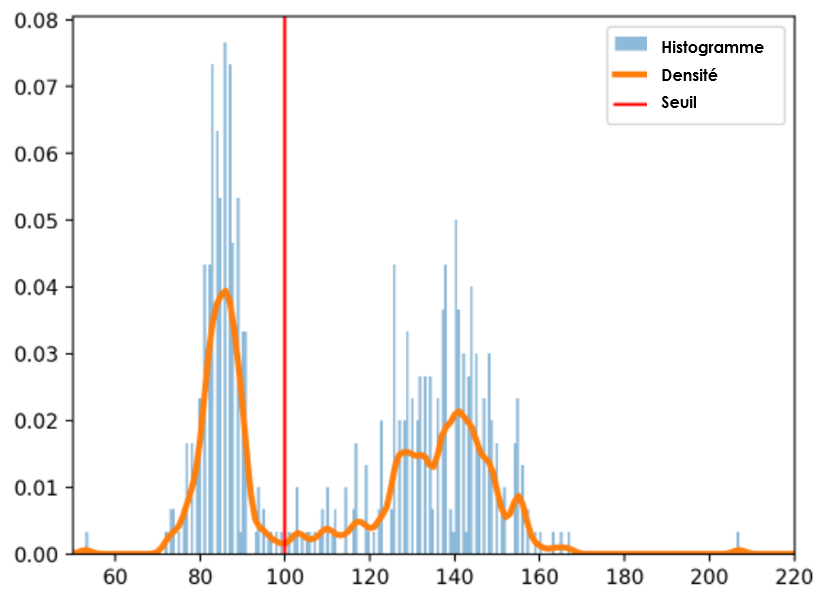
\includegraphics[width=0.8\textwidth]{figures/density_plot.png}
 \caption[Exemple d'histogramme et courbe de densité biopsie ATPase]{Exemple d'histogramme et courbe de densité biopsie ATPase}
 \label{fig:atp_density}
\end{figure}

À partir de ce seuil, il est  possible de classer les fibres musculaires en deux catégories: celles avec une intensité moyenne inférieure au seuil et celles avec une intensité moyenne supérieure. La figure \ref{fig:apt_paint} présente les résultats de la quantification automatique des fibres de l'image présentée en exemple précédemment. Sur cette image, on a pu quantifier au total la présence de 496 fibres, dont 269 (54\%) fibres de type 1 et 227 (46\%) fibres de type 2. 
\begin{figure}[!ht]
 \centering
 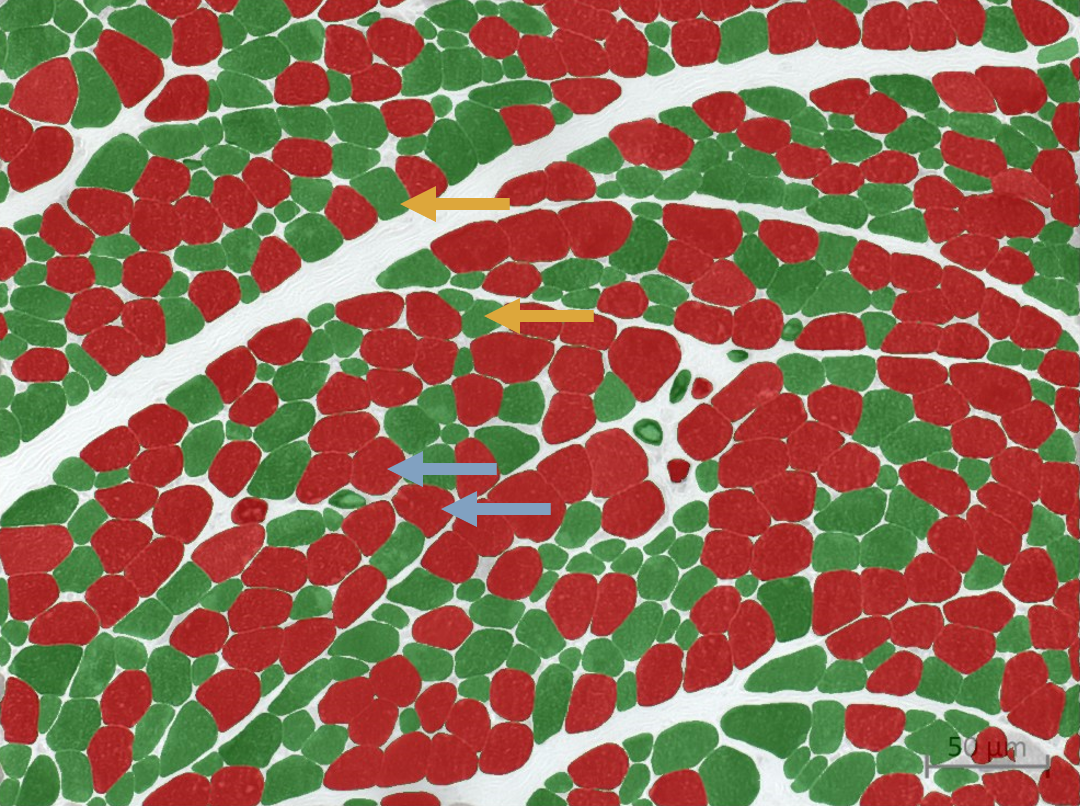
\includegraphics[width=0.8\textwidth]{figures/atp_paint.png}
 \caption[Exemple de classification de biopsie musculaire à la coloration ATPase pH 9.4]{Exemple de classification de biopsie musculaire à la coloration ATPase pH 9.4. Colorer en rouge les fibres ayant une intensité inférieure au seuil (type 2) en vert supérieur au seuil (type 1)}
 \label{fig:apt_paint}
\end{figure}

\subsection{Exemple d'application: classification d'une coupe complète avec trois types de fibres}
La coloration ATPase peut révéler plus de deux types de fibres musculaires. En effet, les fibres de type 2 ont plusieurs sous-types visualisables dans certaines conditions de coloration. Dans cet exemple, nous avons utilisé la méthode de classification développée pour détecter trois types de fibres. L'algorithme présenté dans cette section est capable d'établir autant de seuils automatiquement que spécifiés par l'utilisateur.. La figure \ref{fig:atp_paint_wsi} présente les résultats de classification d'une \gls{wsi} de biopsie musculaire colorée à l'ATP pH 4.6. Sur cette coupe on observe trois populations de fibres: des fibres pâles (fibres de type 2A), des fibres intermédiaires (fibres de type 2B) et de petites fibres très sombres localisées en haut de la coupe (fibres de type 1). La méthode de quantification a alors pu définir deux seuils pour séparer ces trois classes. 
\begin{figure}[!ht]
 \centering
 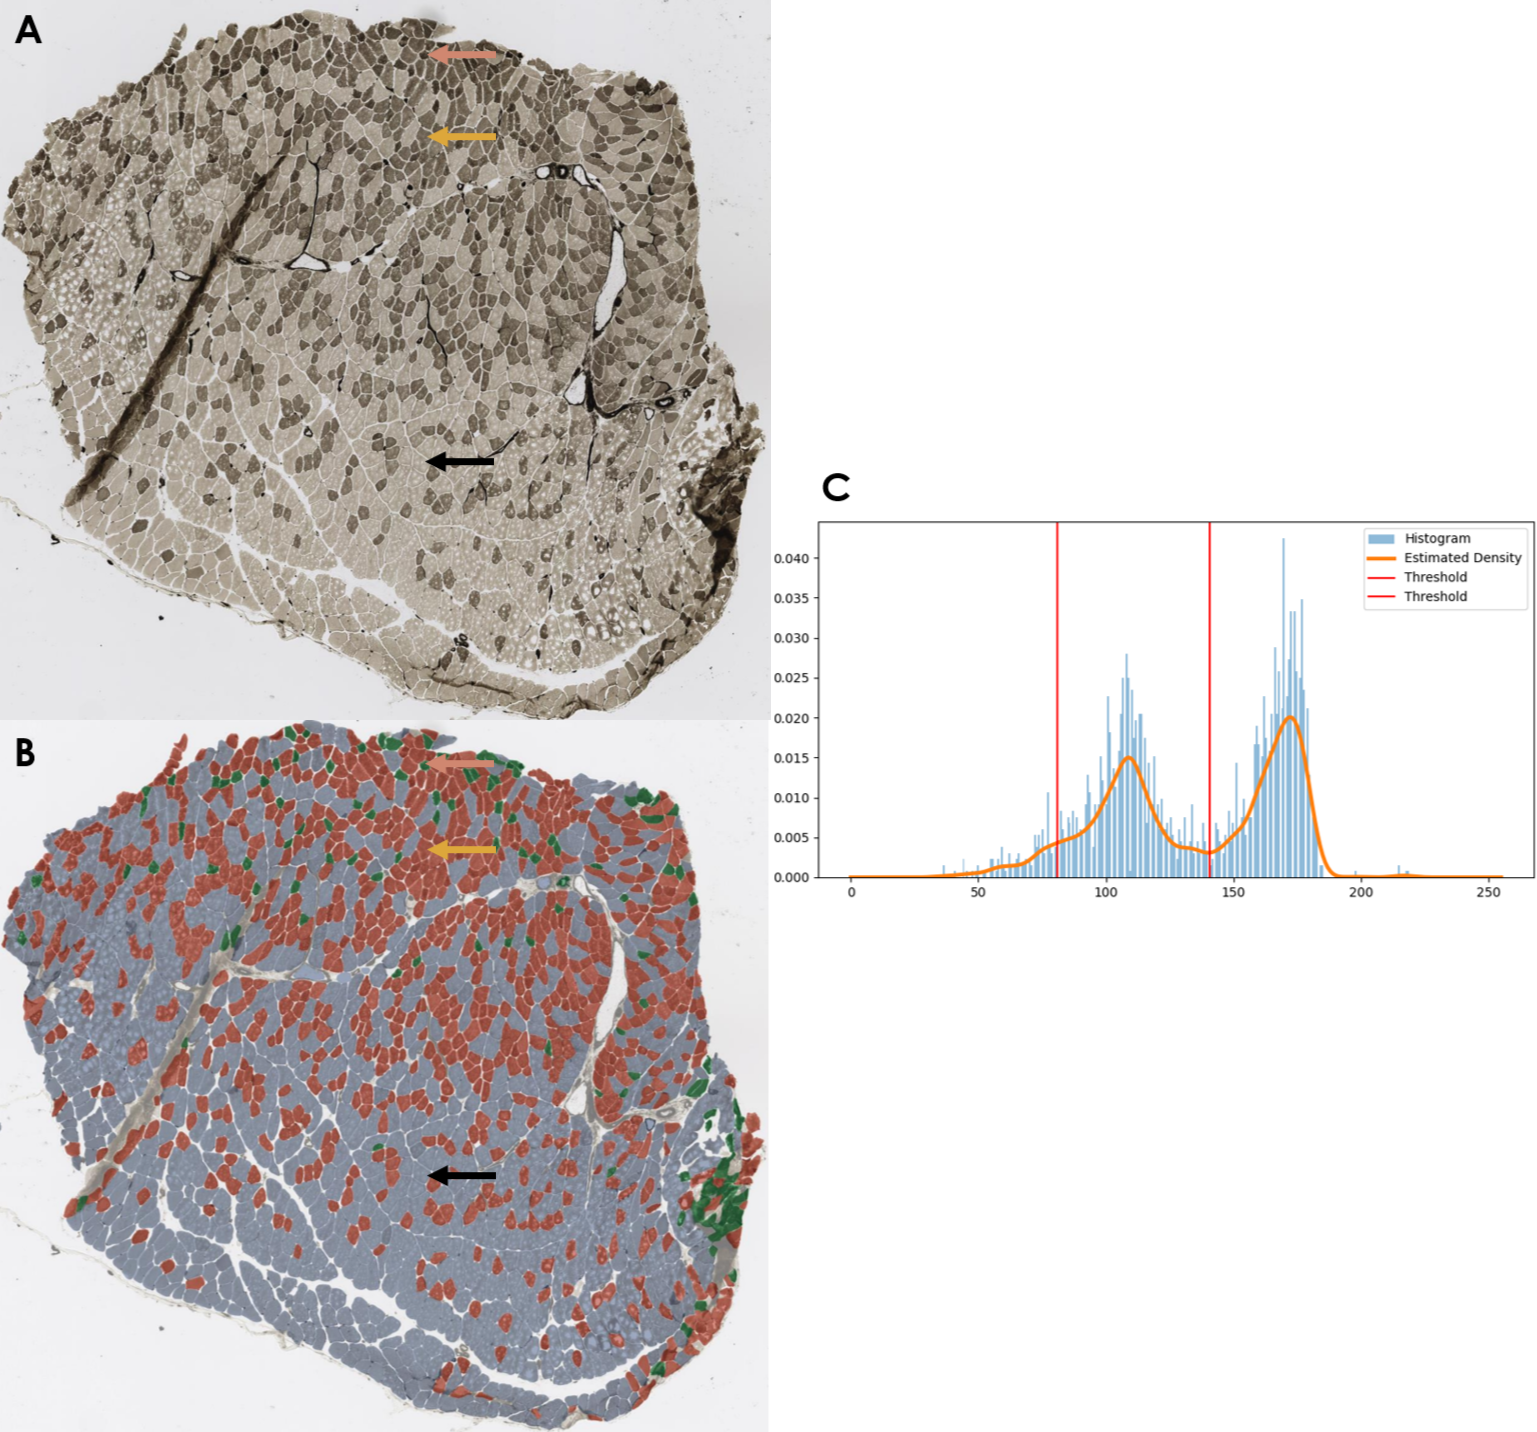
\includegraphics[width=1\textwidth]{figures/atp_wsi.png}
 \caption[Exemple de classification de biopsie musculaire colorée à l'ATPase]{Exemple de classification de biopsie musculaire colorée à l'ATPase en 3 classes: en bleu les fibres de type 2A, en rouge les fibres de type 2B et en vert les fibres de type 1.}
 \label{fig:atp_paint_wsi}
\end{figure}

Les résultats de cette classification sont référencés dans le tableau \ref{tab:atp_wsi_resultstable} , le temps de calcul et la vitesse de classification sont disponibles dans le tableau \ref{tab:atp_wsi_timetable}. Au total, 1840 fibres ont été classifiées en 131 secondes (soit 14 fibres par seconde). Il y a une majorité de fibres de type 2A (894, 49\%), de fibres de type de 2B (829, 45\%) et une faible proportion de petites fibres de type 1 (117, 6\%). Les résultats de cette quantification sont visuellement satisfaisants, bien qu'une partie de la biopsie en bas à droite, est repliée sur elle-même et donc apparaît avec une intensité de coloration forte. Cette zone a donc été considérée à tort comme des fibres de type 1. Ces résultats mettent en évidence le besoin de biopsies avec une préparation de qualité pour obtenir des résultats robustes lors de la quantification automatique.

\begin{table}[!ht]
\centering
\caption{Temps de calcul pour l'analyse des types de fibres d'une coupe complète (1840 fibres, 6000 x 5600 pixels)}
\label{tab:atp_wsi_timetable}
\begin{tabular}{|l|c|c|}
\hline
\textbf{Étape} & \textbf{Temps sur GPU} & \textbf{Fibre par seconde (sur GPU)} \\
\hline
Cellpose & 113 & 16 \\
\hline
Classification des fibres & 18 & 102 \\
\hline
\textbf{Total} & \textbf{131} & \textbf{14} \\
\hline
\end{tabular}
\end{table}
\begin{table}[!ht]
\centering
\caption{Résultats de quantification des types de fibre d'une coupe complète (1840 fibres, 6000 x 5600 pixels)}
\label{tab:atp_wsi_resultstable}
\begin{tabular}{|l|c|c|}
\hline
\textbf{Type} & \textbf{Valeur} & \textbf{Proportion (\%)} \\
\hline
Fibre type 2A & 894 & 49 \\
\hline
Fibre type 2B & 829 & 45 \\
\hline
Fibre type 1 & 117 & 6 \\
\hline
\end{tabular}
\end{table}


\section{Répartition des mitochondries: classification par IA}
Enfin, nous nous sommes intéressés à l'analyse de la répartition des mitochondries dans les fibres musculaires. Cette répartition peut être anormale dans certaines \gls{mc}. Cette répartition se visualise grâce à la coloration \gls{sdh}, révélant l'activité oxydative des fibres musculaires et donc la position des mitochondries. La figure \ref{fig:sdh_example} présente un exemple de biopsie de muscle d'une souris modèle de myopathie congénitale à la coloration \gls{sdh}. On observe deux types de fibres, des fibres "normales" ayant une répartition homogène en coloration et des fibres "anormales" ayant une agglutination de coloration au centre de la fibre (notamment sur la gauche de la coupe), représentant des agrégats mitochondriaux pathologiques. Dans ce cadre, nous avons développé une méthode capable de détecter et de compter les fibres ayant une répartition mitochondriale anormale, en développant notre propre modèle d'\gls{ia}.

\begin{figure}[!ht]
 \centering
 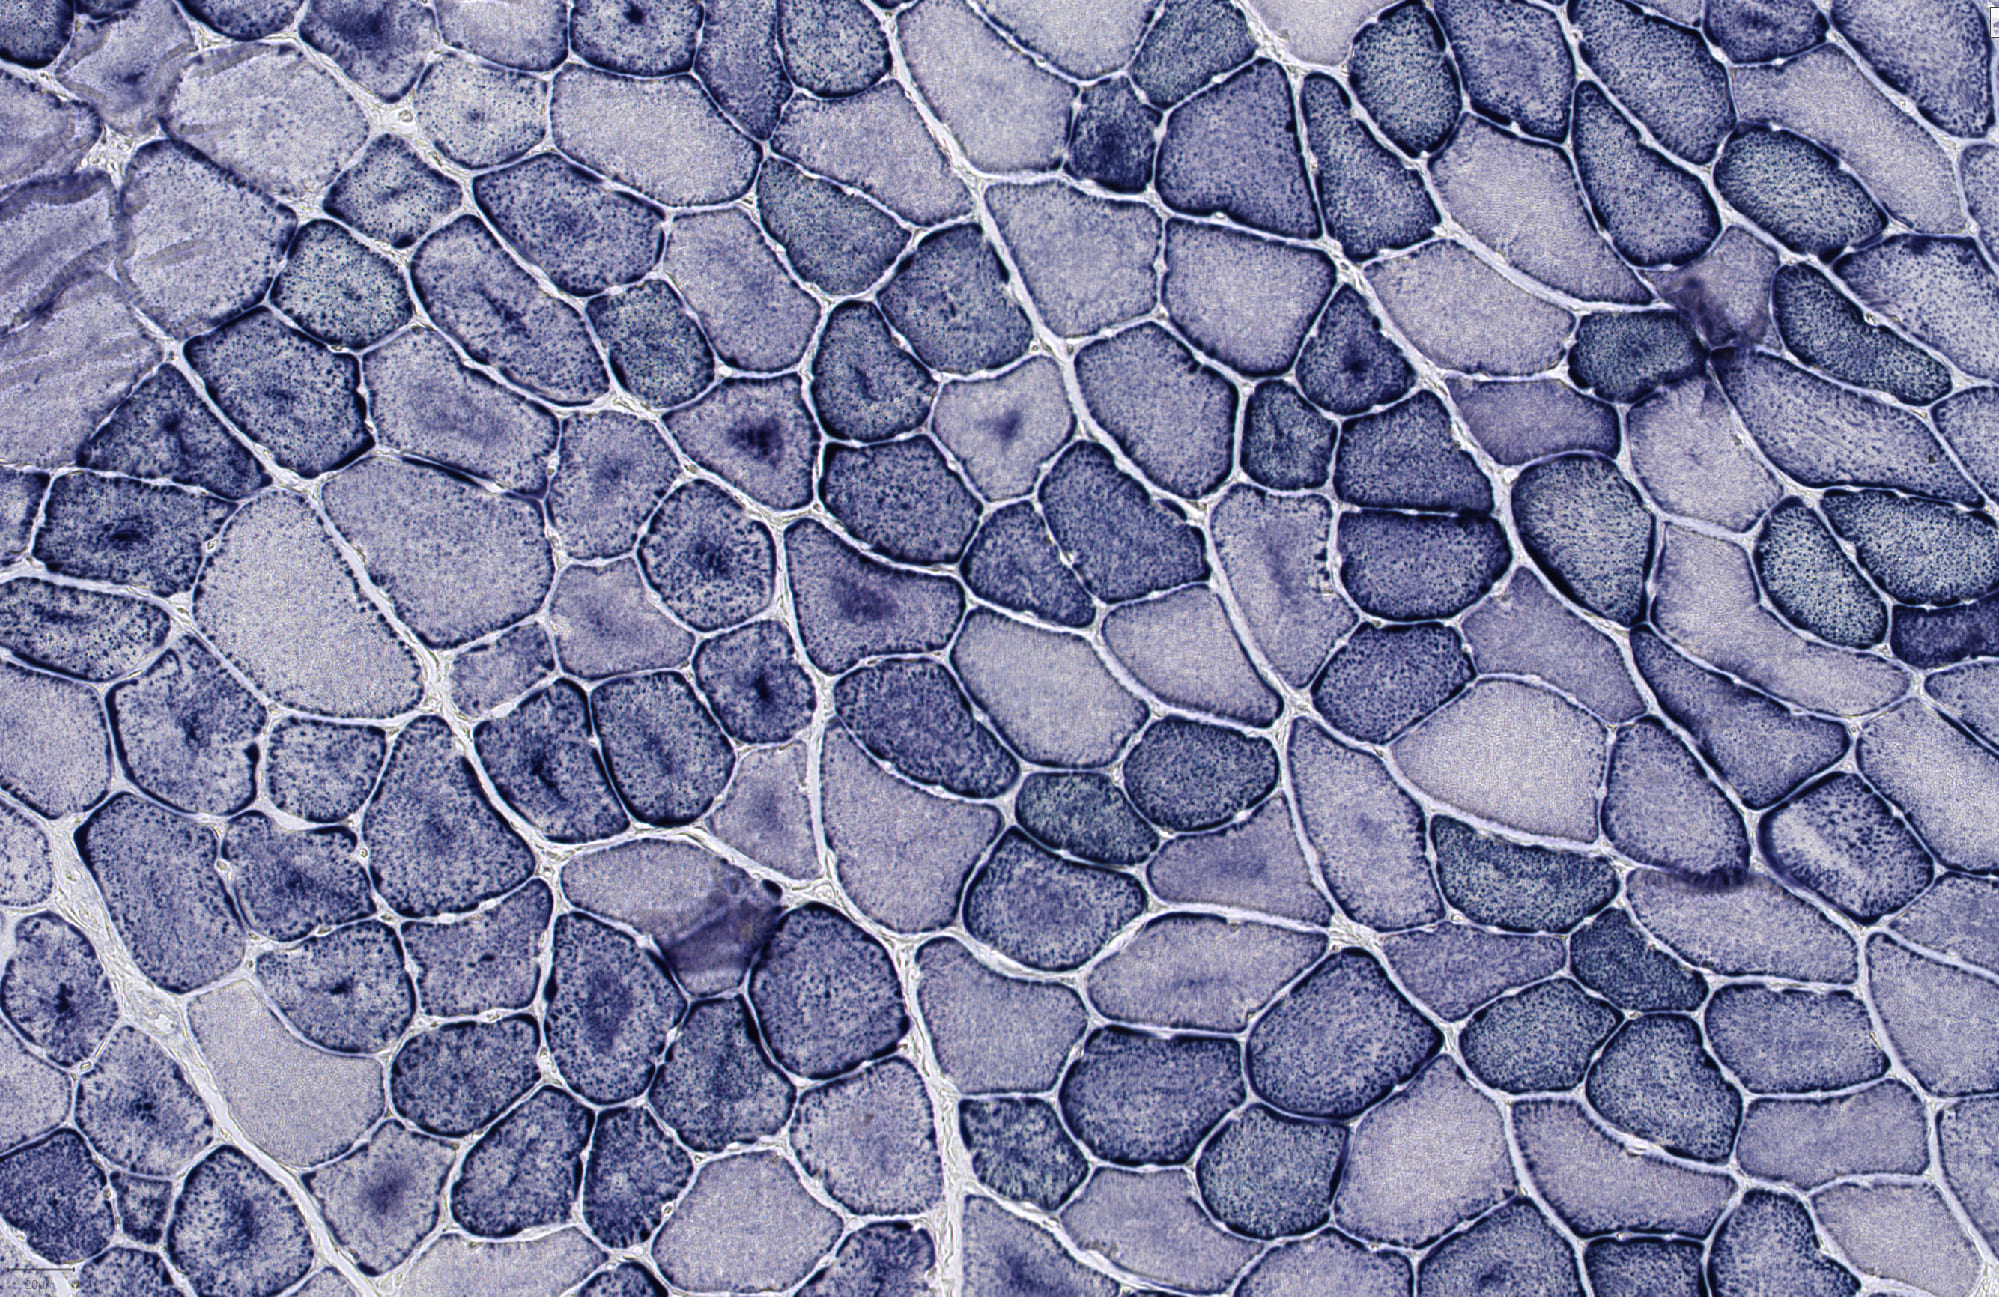
\includegraphics[width=0.8\textwidth]{figures/sdh_example.jpg}
 \caption[Exemple de biopsie musculaire à la coloration SDH]{Exemple de biopsie de muscle de souris modèle de CNM à la coloration SDH}
 \label{fig:sdh_example}
\end{figure}
\subsection{Jeu de données d'image de muscle de souris et annotations}
Pour constituer le jeu de données nécessaire à l'entraînement de cette \gls{ia} nous avons utilisés 18 \gls{wsi} de biopsies musculaires de souris, dont une souris saine (\textit{wild-type}) et 17 \gls{wsi} de souris modèles de \gls{cnm} (10 \textit{Bin1-KO} et 7 \textit{Dnm2S619L}). Ces 18 \gls{wsi} représentent un total de 16 787 fibres musculaires (tableau \ref{tab:sdh_fiber_count}). Chacune de ces fibres musculaires a été isolée et extraite de la coupe grâce à Cellpose puis a été annotée à la main en 2 catégories: fibre saine ou anormale, par l'expert ayant généré les images (Quentin Giraud et Charlotte Gineste). Au total, les 12 730 fibres saines et 4 057 fibres annotées comme anormales ont été séparées équitablement en trois jeux de données: 72\% pour le jeu d'entraînement de l'\gls{ia}, 8\% pour le jeu de validation lors de l'entraînement, et 20\% pour le jeu de test des performances de l'\gls{ia}. Ce jeu de données à été mis à disposition de la communauté scientifique de façon \textit{open-source} sur la plateforme \textit{Hugging-Face} à l'adresse: \href{https://huggingface.co/datasets/corentinm7/MyoQuant-SDH-Data}{https://huggingface.co/datasets/corentinm7/MyoQuant-SDH-Data}.

\begin{table}[!ht]
\centering
\caption{Répartition des fibres pour le jeu d'entraînement du modèle SDH}
\label{tab:sdh_fiber_count}
\begin{tabular}{|c|c|c|c|c|}
\hline
 & \textbf{Entraînement} (72\%) & \textbf{Validation} (8\%) & \textbf{Test} (20\%) & \textbf{Total} \\
\hline
\textbf{Saine} & 9 165 & 1 019 & 2 546 & 12 730 (76\%) \\
\hline
\textbf{Anormale} & 2 920 & 325 & 812 & 4 057 (24\%) \\
\hline
\hline
\textbf{Total} & 12 085 & 1 344 & 3 358 & 16 787 \\
\hline
\end{tabular}
\end{table}


\subsection{Architecture, entrainement et performance du modèle IA}
À partir de ce jeu de données, nous avons entrainé un modèle de \gls{cnn}. Nous avons sélectionné l'architecture réseau de neurones profonds \textit{Resnet50} préentrainée sur \textit{ImageNet}. L'architecture \textit{Resnet50} est une architecture à l'état de l'art pour la classification d'images et le préentrainement sur \textit{ImageNet} permet d'obtenir de meilleures performances et une convergence du modèle accélérée. Pour limiter le surapprentissage, nous avons appliqué des techniques d'augmentation de données lors de l'apprentissage par variation de luminosité, contraste, rotation aléatoire, zoom, translation et retournement. De plus, nous avons utilisé une méthode d'arrêt prématuré pour arrêter l'entrainement lorsque les performances sur le jeu de validation ne se sont pas améliorées lors des 10 dernières époques. Enfin, chaque fibre musculaire unique a été redimensionnée à une taille de 256x256 pixels, car le réseau de neurones impose une taille d'image constante.
\begin{figure}[!ht]
 \centering
 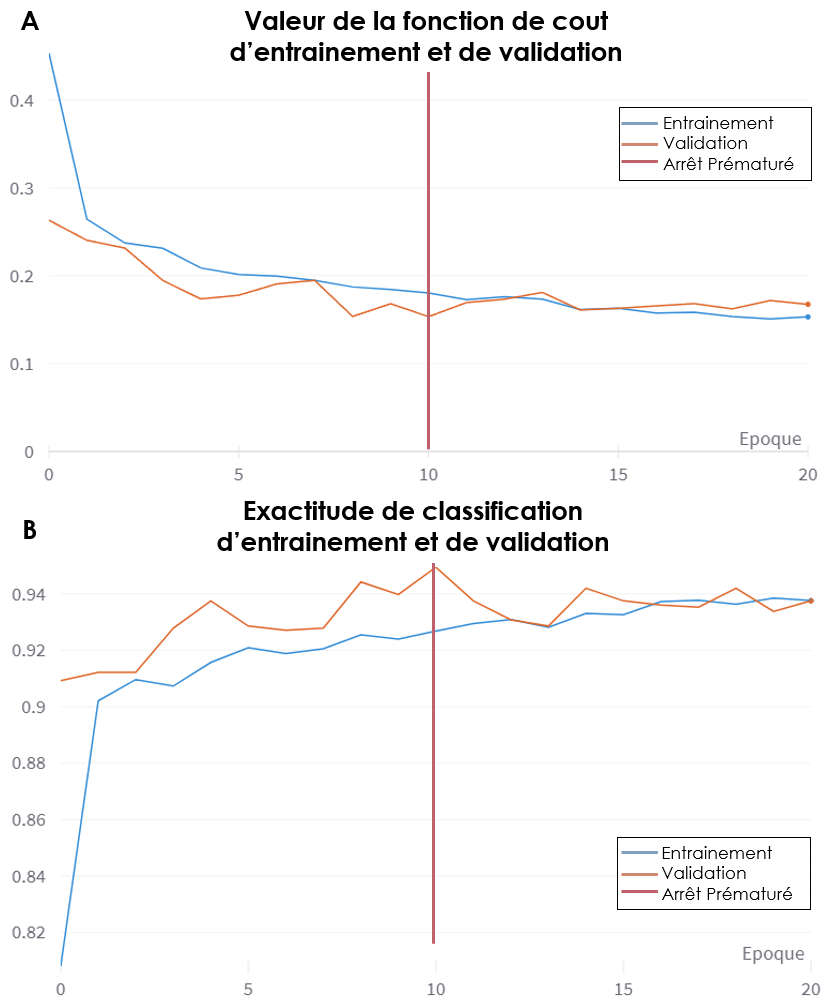
\includegraphics[width=1\textwidth]{figures/training_sdh.png}
 \caption[Courbe d'apprentissage du modèle SDH]{Courbe d'apprentissage du modèle SDH. En haut la courbe d'erreur, en bas la courbe d'exactitude de classification pour le jeu d'entrainement (bleu) et le jeu de validation (orange). La barre verticale rouge indique le modèle final sélectionné par arrêt prématuré.}
 \label{fig:sdh_train}
\end{figure}

La figure \ref{fig:sdh_train} présente les courbes d'apprentissage du modèle \gls{sdh}. Que ce soit en termes de mesure de l'erreur du modèle (\textit{loss}) ou d'exactitude de classification, on observe qu'après 10 époques (12 minutes d'entrainement), les performances sont maximales pour le jeu de validation et ne s'améliorent plus sur les 10 époques suivantes. Ceci indique qu'après 10 époques, l'apprentissage donne lieu à un surapprentissage du jeu d'entrainement. C'est pourquoi grâce à l'arrêt prématuré, nous avons sélectionné le modèle dans l'état après 10 époques comme modèle optimal sans surapprentissage.

Après la phase d'apprentissage, pour mesurer les performances du modèle, nous avons utilisé le jeu de test composé de 3358 images non utilisées pour l'entrainement. En comparant les prédictions du modèle sur les images de test à leur annotation par les experts, nous avons obtenu une exactitude de classification de 93,2\% et une exactitude pondérée de 91.7\%. Autrement dit, le modèle est capable de reproduire l'annotation des deux experts avec une exactitude de 93,2\%.

L'ensemble des métriques mesurées lors de l'entrainement sont disponibles de façon open source à l'adresse: \href{https://wandb.ai/lambda-science/myoquant-sdh/reports/Model-Training---Vmlldzo0NDI4MDI4}{https://wandb.ai/lambda-science/myoquant-sdh/reports/Model-Training---Vmlldzo0NDI4MDI4}, le modèle ainsi que le code source utilisés pour réaliser cet entrainement de manière reproductible sont aussi disponibles sur la plateforme \textit{HuggingFace} à l'adresse: \href{https://huggingface.co/corentinm7/MyoQuant-SDH-Model}{https://huggingface.co/corentinm7/MyoQuant-SDH-Model}.

\subsection{Exemple d'application}
Grâce au modèle développé, il est maintenant possible de classer des fibres individuelles pour détecter les anomalies de répartition mitochondriale. Ainsi pour analyser une image complète, on utilise d'abord Cellpose pour segmenter et isoler chaque fibre musculaire de l'image, puis le modèle que nous avons développé pour prédire la classe de la fibre. Par exemple, pour l'image de biopsie présentée ci-dessus (\ref{fig:sdh_example}), le résultat de classification est présenté en figure \ref{fig:sdh_paint}. Au total, sur 162 fibres détectées, 86 (53\%) sont classées comme ayant une répartition mitochondriale anormale et 76 (46\%) ont une répartition normale. On observe que ce sont bien les fibres ayant une agglutination de coloration au centre de la fibre (agrégats de mitochondries, sur la gauche de la coupe) qui sont classées comme anormales, confirmant le bon fonctionnement du modèle.

\begin{figure}[!ht]
 \centering
 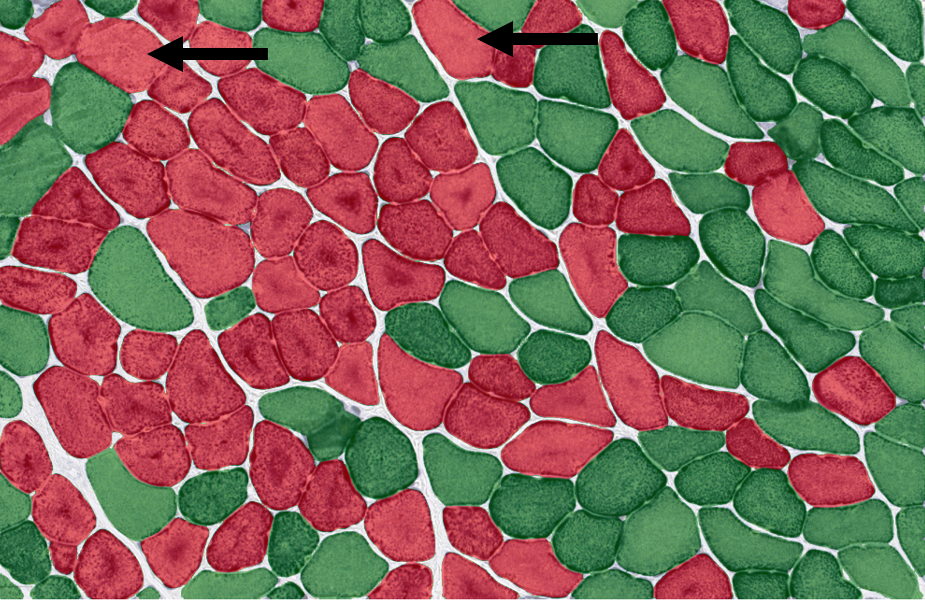
\includegraphics[width=0.8\textwidth]{figures/sdh_paint.png}
 \caption[Exemple de classification de biopsie musculaire de souris à la coloration SDH]{Exemple de classification de biopsie musculaire de souris à la coloration SDH. Colorées en rouge les fibres ayant une répartition mitochondriale anormale, en vert une répartition normale}
 \label{fig:sdh_paint}
\end{figure}
\begin{figure}[!ht]
 \centering
 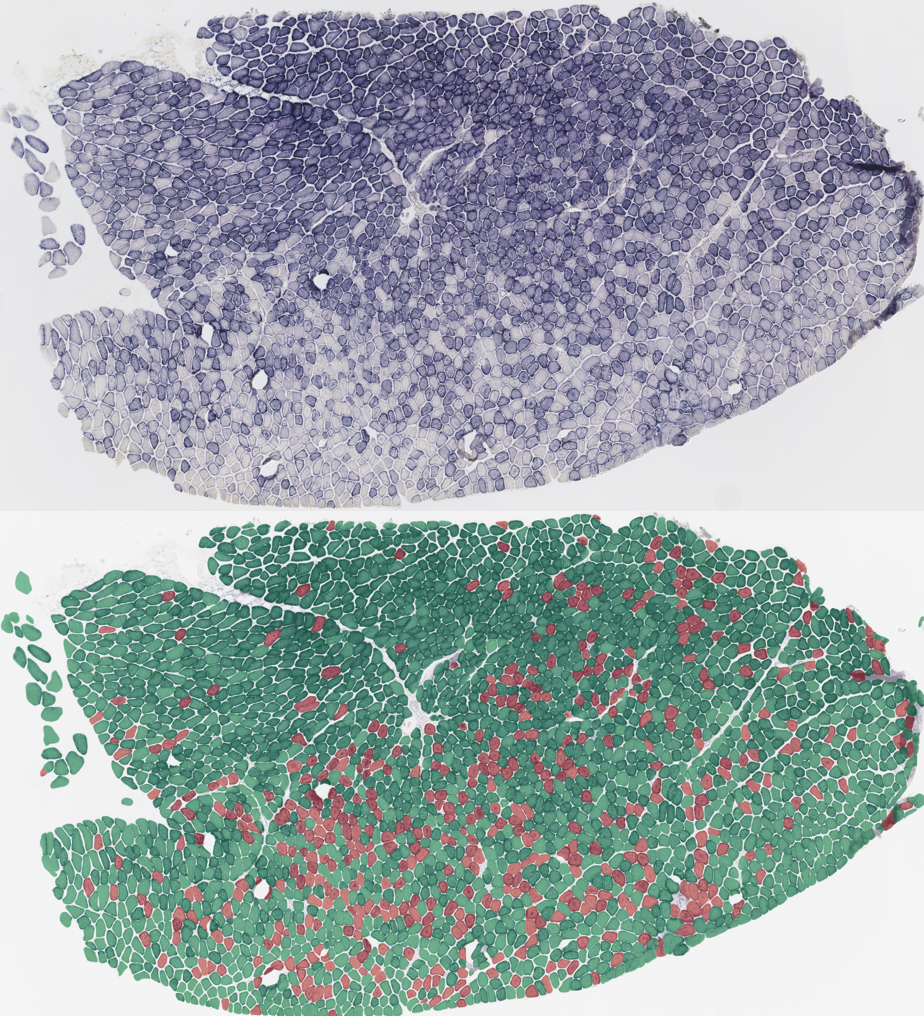
\includegraphics[width=0.8\textwidth]{figures/wsi_sdh.png}
 \caption[Exemple de classification de coupe complète biopsie musculaire de souris à la coloration SDH]{Exemple de classification de coupe complète biopsie musculaire de souris à la coloration SDH. Colorées en rouge les fibres ayant répartition mitochondriale anormale, en vert une répartition normale}
 \label{fig:sdh_wsi_paint}
\end{figure}

Il est aussi possible de classer des \gls{wsi} de biopsies de muscle complet colorées au \gls{sdh}. Par exemple, la figure \ref{fig:sdh_wsi_paint} présente les résultats de classification d'une coupe complète comptant 2 869 fibres musculaires. En termes de ressources de calcul, l'étape limitante reste le modèle Cellpose qui, pour cette image, requiert trop de mémoire pour fonctionner sur notre matériel (\gls{gpu}). Ainsi sur CPU, nous avons eu besoin d'environ 40 minutes pour quantifier la coupe, dont la majorité du temps a servi à Cellpose,  ce qui représente une vitesse d'environ 1 fibre par seconde. Au final sur la coupe présentée, 2371 fibres sont classées comme saines (83\%) et 498 sont classées comme anormales (17\%).

\begin{table}[!ht]
\centering
\caption{Temps de calcul pour l'analyse des fibres d'une coupe complète SDH (2 869 fibres, 11200 x 6300 pixels)}
\label{tab:sdh_wsi_timetable}
\begin{tabularx}{\textwidth}{|l|c|c|X|}
\hline
\textbf{Étape} & \textbf{Temps sur GPU} & \textbf{Temps sur CPU} & \textbf{Fibre par seconde (sur CPU)} \\
\hline
Cellpose & \textit{Mémoire insuffisante} & 2 407 & 1,2 \\
\hline
Classification des fibres & 70 & 66 & 43 \\
\hline
\textbf{Total} & \textbf{>70} & \textbf{2473} & \textbf{1,15} \\
\hline
\end{tabularx}
\end{table}
\begin{table}[!ht]
\centering
\caption{Résultats de quantification des  fibres d'une coupe complète SDH (2 869 fibres, 11200 x 6300 pixels)}
\label{tab:sdh_wsi_resultstable}
\begin{tabular}{|l|c|c|}
\hline
\textbf{Type} & \textbf{Valeur} & \textbf{Proportion (\%)} \\
\hline
Fibres saines & 2371 & 83 \\
\hline
Fibres anormales & 498 & 17 \\
\hline
\end{tabular}
\end{table}


\subsection{Exploration du modèle}
Une fois le modèle entrainé, nous avons voulu explorer le modèle grâce à différentes techniques de visualisation pour nous assurer que ses capacités de classification sont bien réelles et ne sont pas dues à un biais lors de l'apprentissage.

\subsubsection{Explicabilité de la classification}
Afin de vérifier sur quels critères la classification des fibres est réalisée, nous avons utilisé la méthode Grad-Cam (\textit{Gradient-weighted Class Activation Mapping}, \cite{selvaraju_grad-cam_2020}). Cette méthode permet de générer une carte thermique des images pour visualiser les régions importantes pour la classification selon le modèle. Cette carte thermique est réalisée en utilisant les gradients de la sortie par rapport aux cartes de \textit{features} des couches convolutives pour chaque classe, puis une moyenne pondérée est calculée.

\begin{figure}[!ht]
 \centering
 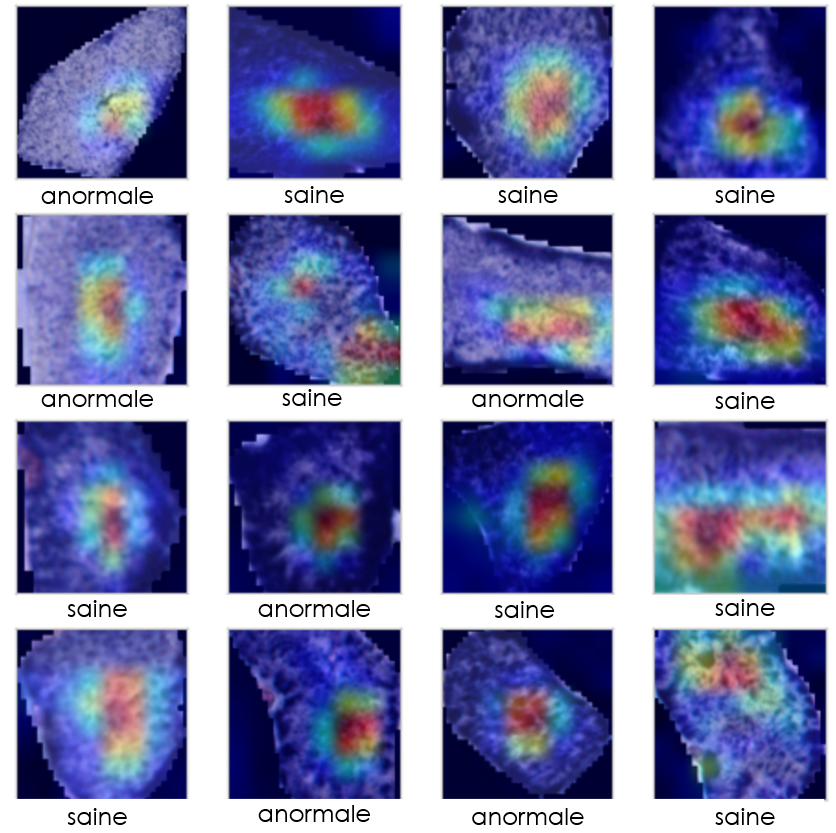
\includegraphics[width=0.8\textwidth]{figures/sdh_gradcam.png}
 \caption[Visualisation par méthode \textit{Grad-Cam} du modèle SDH]{Visualisation par méthode  \textit{Grad-Cam} de la classification de 16 fibres prises au hasard du jeu de test par modèle SDH. Superposition de l'image originale redimensionnée et de la carte thermique générée}
 \label{fig:gradcam_sdh}
\end{figure}
La figure \ref{fig:gradcam_sdh} présente les résultats de cette méthode de visualisation sur 16 fibres musculaires uniques prise au hasard dans le jeu de test. On observe sur cette figure que la zone déterminante pour la classification des fibres selon le modèle est le centre de la fibre musculaire. Cette observation est cohérente, car nous avons observé que dans la majorité des cas, une fibre est dite anormale lorsqu'elle présente une agglutination de coloration au centre de la fibre (agrégats de mitochondries centralisés). Cette résultat/observation... confirme donc que le modèle porte son attention globalement sur la même zone que l'expert lors de la classification manuelle. 

\subsubsection{\textit{Embedding} des images et réduction de dimensionnalité} 
Pour rappel la notion d'\textit{embedding} correspond  à la transformation d'une donnée en un vecteur numérique de grande taille. Dans \gls{nlmyo} nous avons utilisé des techniques d'\textit{embedding} sur des données textuelles. Ici, nous avons réalisé un \textit{embedding} de nos images, non pas pour faire de la classification, mais pour appliquer des techniques de réduction de dimensionnalité (comme une PCA) pour visualiser si notre modèle est bien capable de faire une différence nette entre les deux classes.
Pour cela, nous avons utilisé notre modèle \gls{sdh} et avons retiré la dernière couche de neurones servant à la classification. Ainsi la sortie du modèle correspond à la sortie de la dernière couche convolutive, c'est-à-dire à un vecteur de taille (1, 2048) correspondant aux caractéristiques importantes de l'image extraite par le modèle pour la classification.  En réalisant cette opération pour l'ensemble des images, nous obtenons une matrice (16 787, 2048) sur laquelle nous appliquons une méthode de réduction de dimensionnalité (nommée UMAP (\cite{mcinnes_umap_2020})), donnant ainsi une matrice (16 787, 2) visualisable facilement.
\begin{figure}[!ht]
 \centering
 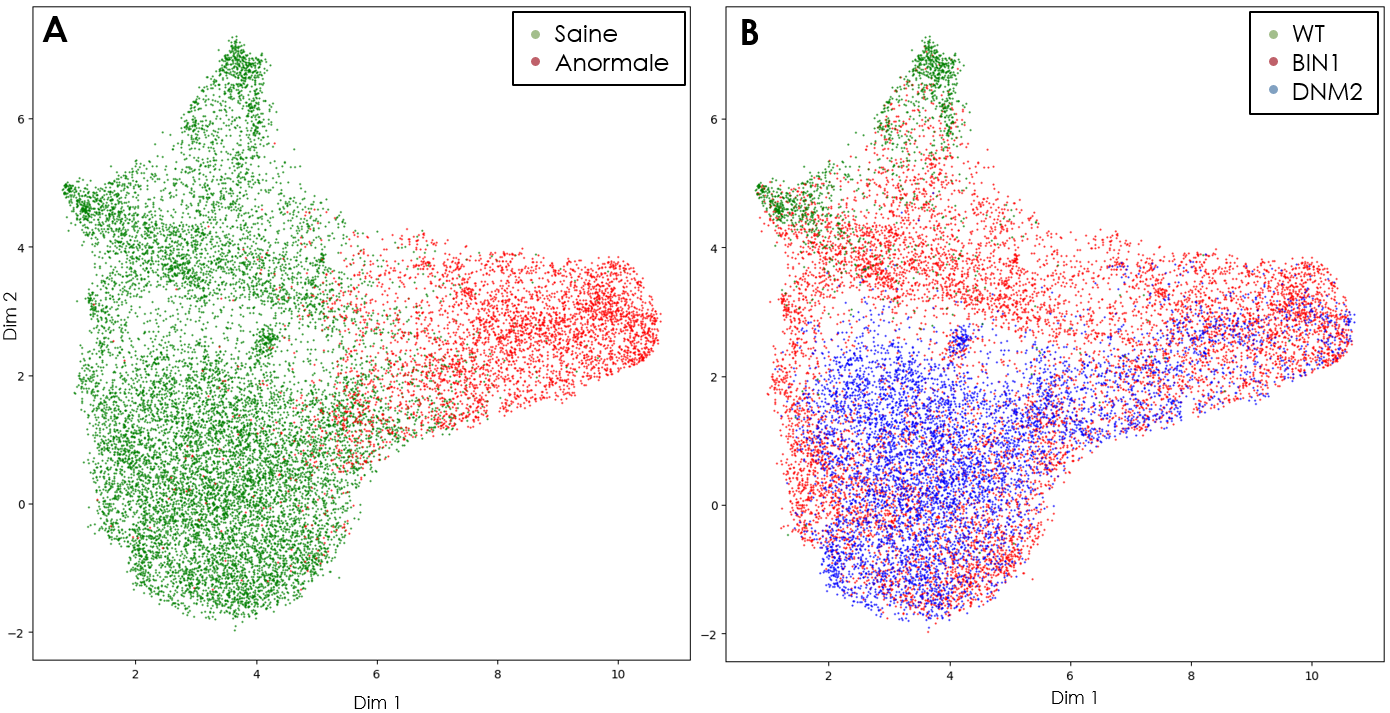
\includegraphics[width=1\textwidth]{figures/umap_sdh.png}
 \caption[Visualisation de l'\textit{embedding} du modèle SDH]{Visualisation de l'\textit{embedding} du modèle SDH des 16 787 images de fibres musculaires après réduction de dimensionnalité par UMAP. À gauche, les fibres sont colorées par label, à droite elles sont colorées par modèle de souris}
 \label{fig:umap_sdh}
\end{figure}

Ainsi, la figure \ref{fig:umap_sdh} présente la visualisation obtenue après \textit{embedding} et réduction de dimensionnalité des 16 787 images du jeu de données. Chaque point représente une image du jeu de données, colorée selon son label (annotation) ou sa provenance (modèle de souris). Globalement on observe que sur le premier (et donc le plus important) axe de variance (en abscisse), le modèle extrait des informations permettant de faire la différence entre les fibres saines et anormales. En effet les deux classes de fibres sont bien séparées avec cependant la présence d'un continuum entre les deux groupes indiquant la présence de fibres avec des profils intermédiaires plus complexes. Le second axe de variance (en ordonné) indique que le modèle extrait aussi des informations permettant d'établir la provenance de la fibre, c'est-à-dire de quel modèle de souris elle est issue. En effet, on voit un cluster de fibres venant de souris \textit{wild-type} assez compact en haut de la figure, puis deux clusters à la fois superposés et séparés de fibres provenant de souris modèle \textit{BIN1} et \textit{DNM2}. L'ensemble des ces résultats confirment que notre modèle extrait et base sa classification des fibres sur les caractéristiques intrinsèques des fibres saines ou anormales et non, sur des biais extérieurs.

\subsubsection{Identification des erreurs d'annotation par le modèle}
Lors de la phase de test, le modèle a obtenu une exactitude de classification de 93.2\%, il existe donc une marge de progression pour le modèle. Les 6.8\% d'erreur peuvent être expliqués par plusieurs raisons. La première est que le modèle n'est peut-être pas assez complexe pour capturer l'ensemble des critères de classification des images et donc a des difficultés pour certains cas complexes. Cependant cette explication a peu de chance d'être fondée car nous utilisons un modèle à l'état de l'art \textit{Resnet50} avec plus de 25 millions de paramètres, ce qui devrait être largement suffisant pour cette tache de classification. Un seconde raison pourrait être la présence de bruit ou d'erreurs dans le jeu de données de base. Nous avons alors exploré comment nous pouvions, grâce au modèle entrainé, le jeu de données initial pour potentiellement trouver des erreurs d'annotation.

La figure \ref{fig:identify_errors} résume la démarche utilisée pour identifier des erreurs dans le jeu de données. À partir de la prédiction de la classe des 16 787 images, nous avons filtré pour ne garder que les images où le label (annotation par l'expert) était discordant avec la prédiction du modèle ET où le modèle avait un fort niveau de confiance dans la prédiction (>85\%). Au total cela représente 228 images, soit 1.66\% du jeu de donnée de base.
\begin{figure}[!ht]
 \centering
 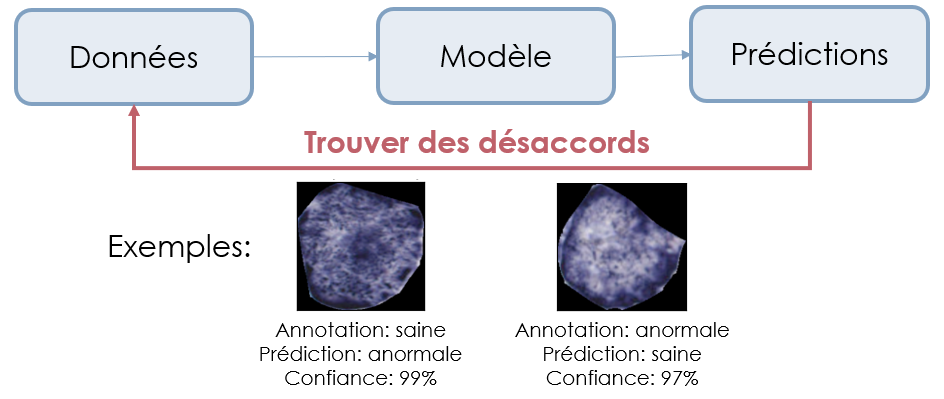
\includegraphics[width=1\textwidth]{figures/identify_errors.png}
 \caption[Méthode d'identification des potentielles erreurs d'annotation]{Méthode d'identification des erreurs d'annotation potentielles }
 \label{fig:identify_errors}
\end{figure}

La figure \ref{fig:list_errors} présente huit exemples pris au hasard parmi les 228 images ayant une prédiction discordante avec l'annotation et un haut niveau de confiance du modèle. On observe par exemple pour la première et la dernière image, qu'elles ont été annotées par l'expert comme saines et prédites comme anormales par le modèle. En regardant l'image de la fibre, on observe une tache centrale caractéristique de fibres ayant une répartition mitochondriale anormale. Ceci laisse donc penser qu'il y a eu une erreur d'annotation pour ces deux fibres, considérée à tort comme saine. De même, pour la seconde image, annotées comme anormale, mais prédite comme saine, on observe la présence d'un marquage homogène sans agglutination caractéristique du marquage au centre, il n'y a donc visiblement pas de raison pour la classer comme anormale.

Ces résultats montrent que le modèle est capable après entrainement d'identifier des erreurs humaines lors de l'évaluation des fibres. Ces erreurs d'annotation peuvent être dues à des inattentions ou des erreurs de clic lors du travail manuel et répétitif d'annotation des  16 787 images par les experts. La détection de potentielles erreurs par le modèle et leur réannotation pourrait permettre d'améliorer le jeu de données utilisé pour l'entrainement du modèle et ainsi obtenir de meilleures performances de classification.
\begin{figure}[!ht]
 \centering
 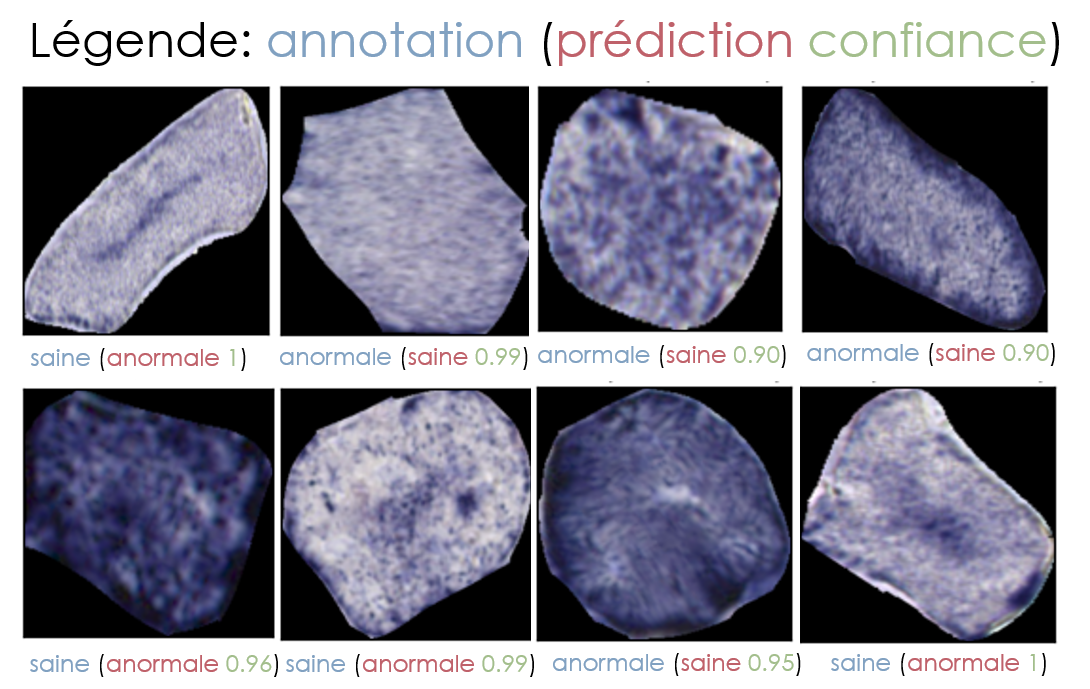
\includegraphics[width=1\textwidth]{figures/list_sdh_errors.png}
 \caption[Exemple de fibres ayant un label prédit contraire a l'annotation avec un haut niveau de confiance du modèle]{Exemple de fibres ayant un label prédit contraire à l'annotation avec un haut niveau de confiance du modèle}
 \label{fig:list_errors}
\end{figure}

\section{Déploiement de la plateforme}
Pour faciliter l'utilisation et la diffusion de \gls{myoquant}, nous avons développé l'outil sous deux formes: un outil en ligne de commande et une version de démonstration en ligne.

\subsection{Outil en ligne de commande}
Sous sa forme d'outil en ligne de commande, \gls{myoquant} est téléchargeable comme bibliothèque Python disponible dans le répertoire officiel PyPI à l'adresse \href{https://pypi.org/project/myoquant/}{https://pypi.org/project/myoquant/}. La version en ligne de commande permet de traiter un grand nombre d'images et/ou des images de coupes complètes trop grandes pour être traitées via une interface en ligne. Ceci permet de traiter les images sur des serveurs de calcul équipés de \gls{gpu} afin d'accélérer le processus d'analyse et de sauvegarder l'ensemble des résultats.

\subsection{Version de démonstration en ligne}
\gls{myoquant} est aussi disponible sous forme d'interface de démonstration en ligne développée grâce à \textit{Streamlit}. Cette interface en ligne est utile pour faire des démonstrations de l'outil de façon visuelle, notamment grâce aux différents graphiques d'explicabilité générés. Cette interface permet aussi de tester l'outil sur des images de petites tailles afin d'évaluer quels seraient les meilleurs paramètres pour obtenir une classification de qualité. \gls{myoquant}-Streamlit est disponible en ligne à l'adresse \href{https://lbgi.fr/MyoQuant/}{https://lbgi.fr/MyoQuant/} ainsi que sur \textit{HuggingFace Space} \href{https://huggingface.co/spaces/corentinm7/MyoQuant}{https://huggingface.co/spaces/corentinm7/MyoQuant}.

\section{Limites et perspectives de développement}
L'outil \gls{myoquant} permet de quantifier des marqueurs pathologiques dans trois des cinq colorations réalisées en routine pour le diagnostic des \gls{mc}. Pour l'instant, \gls{myoquant} n'inclus pas de méthode dédiée à l'analyse des coupes à la coloration \gls{tg} pour détecter les agrégats protéiques, ni de méthode pour la coloration NADH pouvant mettre en évidence la présence de \textit{cores}. Des modèles \gls{ia} suivants la même méthodologie que ce que nous avons développé pour la coloration \gls{sdh} devront être développés en conséquence. Il est aussi nécessaire pour certaines colorations d'élargir le champ des marqueurs pathologiques quantifiés. Par exemple, pour la coloration \gls{he}, la taille des fibres pour  la détection de fibres atrophiques est aussi évaluée en routine lors du diagnostic en complément de la position des noyaux.

De plus, \gls{myoquant} a majoritairement été développé à partir de données issues de biopsies musculaires de souris. Il serait intéressant de tester \gls{myoquant} sur un jeu de données de biopsies humaines quantifiées manuellement par un expert pour évaluer son niveau de performance sur des données humaines. En cas de performance satisfaisante, il serait alors possible d'analyser de façon massive les données de patients afin d'établir de potentiels seuils pour chaque marqueur pathologique pour le diagnostic automatique de \gls{mc}.

 Enfin, sur un plan technique, il serait intéressant de développer une interface en ligne pour \gls{myoquant} liée à des \gls{gpu} pour le traitement de coupes complètes en un temps raisonnable sans avoir à utiliser la ligne de commande, qui est un frein majeur pour un public non expérimenté en programmation, ce qui est typiquement le cas lors du diagnostic.
\part{DISCUSSIONS}
\chapter{Discussions et ouvertures}
Dans les chapitres précédents nous avons présenté les trois outils (\gls{impatient}, \gls{nlmyo} et \gls{myoquant}) que nous avons développé pour exploiter les données multimodales de patients atteints de myopathies congénitales. Bien que ces méthodes soient fonctionnelles, elles présentent des challenges et des perspectives d'amélioration à la fois biologiques et techniques. Au niveau biologique (interprétation des résultats), nous allons discuter de l'intégration des données génomiques comme modalité supplémentaire ainsi que de la question de la mise en relation des différentes modalités entre elle (clinique, histologique et génétique). Au niveau technique, il est important d'aborder la question de l'explicabilité des systèmes \gls{ia}, des ressources nécessaires à la mise en place de système \gls{ia} et des aspectes législatifs de la mise en place de tel système pour le traitement de données de santé. Enfin une dernière perspective de valorisation des travaux sera abordée concernant l'intégration des outils dans un projet de création de produit combinant les outils en un seul point d'accès unique.

\section{Intégration de nouvelles modalités de données: les données génomiques}
Les outils développés se sont concentrés majoritairement sur l'exploitation des comptes rendus médicaux et des données de type imagerie. Le traitement des données génomiques dans le système\gls{impatient} est sommaire: il est possible d'associer un gène muté responsable de la maladie (et une mutation) pour un patient et de filtrer les symptômes en fonction du gène muté d'intérêt. Cependant dans les maladies rares et génétiques, une difficulté majeur est justement de trouver la mutation causant la maladie, pour rappel, 50\% des patients atteint de myopathie congénitale n'ont pas diagnostic génétique à ce jour. Ainsi il serait intéressant d'ajouter au panel d'outils développés ici des outils capable d'analyser des données de séquençage pour détecter et prioriser des mutations potentiellement responsables de maladie génétique. 

Par exemple, la figure \ref{fig:variant_discuss} présente une façon d'intégrer les données génomiques. L'utilisateur pourrait joindre au dossier du patient un fichier VCF listant les variants trouvés dans son génome. A partir de cette liste, il serait possible de filtrer les variants pour ne garder que les variants liés aux gènes des myopathies congénitales puis de classer les variants par niveau de pathogénicité (en intégrant des outils de prédiction de pathogénicité comme MISTIC (\cite{chennen_mistic_2020})). Enfin il serait possible de prioriser les variants de cette liste en croisant la liste avec les données phénotypiques et histologiques. Par exemple dans le cadre des myopathies à némaline, la présence de bâtonnets dans les fibres musculaires est souvent liée à une mutation dans les gènes NEB, TPM2, TPM3 ou ACTA1. Ainsi on pourrait filtrer la liste de variants pour ne conserver que les variants pathogènes dans ces gènes. Cette approche pourrait permettre filtrer rapidement de potentiels variants responsables de la maladie génétique du patient.

Cependant la recherche exhaustive de variants génétiques par séquençage complet du génome n'est pas universellement disponible en France et donc les données sont limitées. Des initiatives comme le Plan France Médecine Génomique 2025 visent à démocratiser la médecine génomique pour le diagnostic des patients.
 \begin{figure}[htbp]
 \centering
 
\includegraphics[width=1\textwidth]{figures/variant_discuss.png}
 \caption[Exemple de méthode d'intégration des données génomiques]{Exemple de méthode d'intégration des données génomiques}
 \label{fig:variant_discuss}
\end{figure}

\section{Mise en relation des modalités}
Jusque ici nous avons traité les différentes modalités des données dans les maladies rares (données cliniques, histologiques et génétiques) séparément, par une approche en silo. Nous avons utilisé cette approche en raison de la nature parcellaire et fragmentée des données que nous avions à disposition et du mélange données humains (rapport de biopsie) et données de souris (coupe histologiques de modèle de \gls{mc}). Cette approche bien qu'utile, limite nos capacités à réaliser des découvertes transversales à partir de données multimodales. En effet chaque type de données ne révèle qu'une facette de la maladie. 

Il est probable que ce n'est que par le croisement des différentes modalités que l'on puisse accéder à une meilleure compréhension des myopathies congénitales. Par exemple, une caractéristique clinique pourrait être observée plus fréquemment chez des patients avec un profil histologique et génétique particulier. La détection de tel interaction pourrait permettre un diagnostic facilité et plus rapide sur la simple base des symptômes cliniques.

Pour cela, il est nécessaire de constituer un jeu de données à haute valeur ajoutée. Ce jeu de données comprendrait une cohorte de patients pour lesquels les informations cliniques, histologiques et génétiques complètes aient été récupérées. L'analyse de ce jeu de données avec les outils développés ici pourrait permettre de découvrir des corrélations de phénotypes entre les modalités, d'établir des seuils pour les marqueurs pathologiques quantifiés et de mettre en évidence des critères discriminants pour le diagnostic des myopathies congénitales.

\section{Explicabilité et exploration des données patient}
L'explicabilité des modèles d'\gls{ia} est un enjeu majeur notamment en médecine quand ces modèles sont employés pour le diagnostic. Parmi les méthodes que nous avons développées, le niveau d'explicabilité est variable.

La plateforme d'annotation et d'exploration\gls{impatient}, qui est relativement coûteuse en travail manuel de mise en forme des données, offre l'avantage de permettre une classification par \gls{ia} transparente et explicable. Comme vu dans le chapitre 5 et 6, l'importance de chaque symptôme dans le cadre d'un modèle de classification peut être évaluée, ce qui permet une confiance accrue dans les prédictions.

\gls{myoquant} utilise des réseaux de neurones profonds pour la quantification, ces réseaux sont en général considérés comme des boites noires. Cependant ici, le réseau de neurones n'est pas utilisé pour faire du diagnostic mais pour extraire et quantifier des marqueurs pathologiques sur lesquels les prédictions peuvent être réalisées. Ainsi on a un système explicable car le système en boite noire n'est utilisé que pour quantifier des symptômes, ce qui est vérifiable à tout moment en comptant manuellement.

Cependant concernant \gls{nlmyo}, qui repose sur les \gls{llms}, l'explicabilité est moindre. En effet le système de classification de \gls{nlmyo} repose sur les modèles \gls{llms} d'\textit{embedding} qui sont des boites noires totales, la signification des valeurs du vecteur issue des modèles d'\textit{embedding} est inconnue. Le système permet donc une classification automatique et instantanée, mais il n'est pas transparent ni explicable: il est impossible de savoir sur quels critères la classification a été réalisée.

Les recherche en terme d'explicabilité doivent se poursuivre, notamment pour envisager l'utilisation de modèles \gls{ia} pour réaliser de l'aide au diagnostic. Dans cette thèse nous avons exploré trois niveaux d'explicabilité via les différentes méthodes développées. Une solution mise en place ici pour utiliser les modèles de réseau de neurones, considéré comme des boites noires, a été de les utiliser pour faire simplement de l'extraction et quantification de marqueurs (\gls{myoquant}). Concernant les modèles de langage, une solution au problème de boite noire serait de ne pas les utiliser pour faire de la classification mais pour faire de l'extraction de symptômes (et donc pour annoter les patients) et réaliser la classification à partir de ces annotations par \gls{xai}.

\section{Ressources informatiques et déploiement de méthodes IA}
Les approches \gls{ia} révolutionnent la façon d'exploiter les données biomédicales. Cependant elles représentent un coût en calcul important qui mis en évidence un challenge technique pour la mise en place de telle approche.

En terme d'analyse d'images, notamment pour les images histologiques, la taille des images à analyser sont particulièrement importantes. Ainsi sur une machine classique, avec un processeur (CPU) et sans\gls{gpu}, l'analyse risque d'être bien trop lente.  De plus, la taille des images histologiques peut souvent être importante au point de dépasser la mémoire disponible sur les \gls{gpu} classiques. Cette grande taille des images histologiques, induit la nécessite de matériel ou de méthode spécifiques, capables de gérer des volumes de données importants.

Pour l'analyse de texte, les \gls{llms} comme leur nom l'indique sont des modèles très grands et lourds à héberger (plus de 170 milliards de paramètres pour \textit{GPT-3}). Ils requièrent donc du matériel spécialisé et coûteux, c'est à dire plusieurs \gls{gpu} haut de gamme. Cependant les efforts d'optimisation en cours comme la \textit{quantisation} sur 4 bits ont permis de réduire les ressources nécessaires pour héberger de tel modèles. En seulement 2 mois après la sortie de grands modèles \textit{open-source} comme \textit{LLaMA}, il est maintenant possible d'héberger ces modèles de langages sur des machines avec seulement 8 GO de RAM. Ces modèles plus petits et optimisés ont cependant un coup: un qualité de résultats réduite et un temps de génération plus long, les rendant difficilement utilisables en routine. Cependant, nous espérons que ces progrès continueront avec un rythme soutenu, rendant ces modèles de plus en plus accessibles.

En règle générale, les modèles \gls{ia} restent difficile à distribuer et à déployer. L'écosystème informatique nécessaire pour héberger et faire tourner des modèles de réseaux de neurones profonds en production reste complexe et peut être difficile à gérer et à maintenir. Plutôt qu'un système distribué où chaque client pourrait faire tourner ses modèles,  un système centralisé qui mutualise une installation des modèles et les ressources nécessaires à leur fonctionnement serait bénéfique et plus viable à long terme en terme de coûts, stabilité et maintenance.

\section{RGPD et traitement de données de santé}
La solution aux difficultés de l'hébergement des modèles IA peut être l'utilisation d'hébergeurs externes. Par exemple, pour les \gls{llms}, des fournisseurs de modèles et d'hébergement comme \textit{OpenAI} via leur \gls{api} permettent d'utiliser ces modèles sans avoir besoin de ressources de calcul, par facturation à la requête. Toutefois cette solutions présentent un challenge majeur: la confidentialité des données.

En particulier dans le domaine de la santé, les données font l'objet d'un traitement spécifique à cause de leur sensibilité. Leur hébergement et traitement demande un haut niveau de confidentialité et de protection. En particulier en Europe, le \gls{rgpd} qui assure la protection de données personnelles, requiert des exigences strictes en termes de sécurité pour le traitement des données de santé. Ces règles ne concernent pas que les données directement identifiantes comme les noms, et dates de naissance mais aussi des données considérées comme potentiellement identifiantes: résultats génétiques, images histologiques, profile phénotypique.

La nécessité de l'application du \gls{rgpd} représente un frein dans la mise en place et l'hébergement de modèles \gls{ia} innovants pour le recherche biomédicale auprès des équipes de recherche. En effet en plus des sécurités de base nécessaires à l'hébergement de données de santé comme le chiffrement, il est nécessaire de pouvoir faire tourner les modèles \gls{ia} de manière locale, ce qui est techniquement difficile. En cas d'utilisation de fournisseurs externes, il faut établir des contrats de conformités au \gls{rgpd} pour garantir le respect de la protection des données, ce qui n'est pas toujours possible ou coûteux en temps et en argent.

Malgré l'ensemble de ces défis, il est donc important de penser une organisation des outils \gls{ia} permettant d'être conforme aux législations pour permettre de tirer parti des bénéfice de l'\gls{ia} appliquée au domaine biomédical.

\section{Valorisation des travaux: intégration des outils en un point d'accès unique}
Dans l'optique de valoriser les travaux présentés dans cette thèse et de démocratiser l'utilisation de l'\gls{ia} pour l'analyse des données biomédicales, il est nécessaire d'intégrer l'ensemble des outils développés en un point d'accès unique. Cette vision a été encouragée par la \textit{SATT Connectus} à travers le challenge \textit{Mature your PhD} visant à transformer les travaux de recherches en produits innovants.

L'objectif principal est de concilier les trois outils \gls{impatient}, \gls{nlmyo} et \gls{myoquant} en une plateforme unique pour faciliter leur utilisation par les chercheurs. Ainsi l'application web et la base de données \gls{impatient} pourrait servir de pilier de base avec l'intégration de \gls{nlmyo} et \gls{myoquant} pour accélérer l'analyse des données.

Ce projet mets en évidence des défis majeurs déjà identifiés dans les sections ci-dessus, notamment concernant les besoins en ressources de calculs des modèles \gls{ia}, la complexité technique de leur maintenance et les questions de confidentialité des données au regard du \gls{rgpd}. Cependant, pour relever ces défis, il serait possible de structurer cette plateforme en deux parties: un client et un point central de calcul.
 \begin{figure}[htbp]
 \centering
 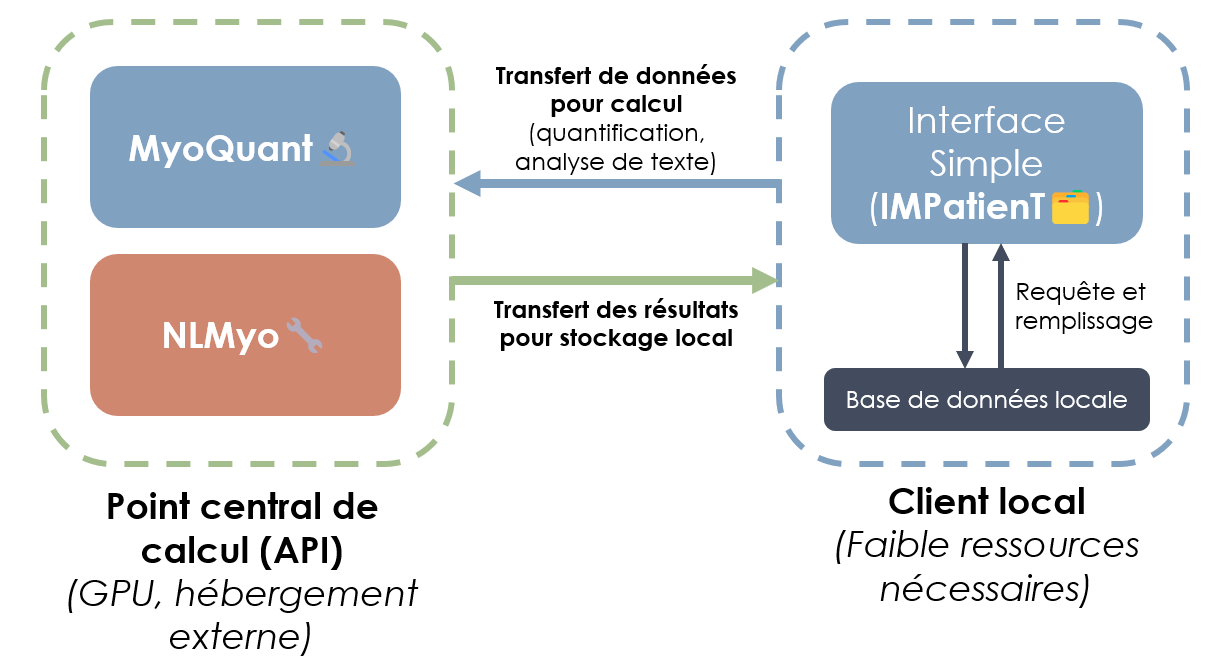
\includegraphics[width=1\textwidth]{figures/perspective_unique.png}
 \caption[Architecture de la plateforme unique en deux parties]{Architecture de la plateforme unique en deux parties. Un client local servant d'interface de hébergeant les donénes et un serveur de calcul disant mutualisé mettant à disposition les modèles IA et les ressources de calculs nécessaires.}
 \label{fig:perspective_unique}
\end{figure}

La figure \ref{fig:perspective_unique} présente l'architecture prévue pour la plateforme unifiée. Le client serait une interface simple permettant d'interagir avec une base de donnée hébergée localement chez le client afin de maintenir la confidentialité et le contrôle des données. A partir de cette interface, il serait possible d'ajouter des patients et de lancer des analyses des données enregistrées (quantification d'images par \gls{myoquant}, ou analyse de texte par \gls{nlmyo}). Ces analyses de données seraient alors déléguées au point central de calcul. Ainsi le client transférerais uniquement les données nécessaires à l'\gls{ia} aux point central de calcul, qui, quant à lui, fournirait les résultats à stocker localement au client.

Cette architecture est adaptée car elle permet à la fois de garantir la confidentialité des données, donnant le contrôle total de leurs données aux chercheurs. Mais aussi elle permet de mutualiser les coûts en ressources informatiques des modèles \gls{ia} avec un point central pour plusieurs clients, dont le déploiement et maintenance serait assurée par notre expertise. Au final cette architecture adaptée en deux parties, qui intègre les trois outils présentés dans cette thèse, permet à la fois de répondre aux challenges techniques tout en facilitant l'utilisation d'\gls{ia} au service de l'analyse des données biomédicales pour les chercheurs.
\printbibliography
\appendix
% \chapter{...}
% ...


\backmatter
\checkoddpage
\ifoddpage
    \mbox{}\newpage % If current page is odd, insert a blank page
\else
    % If current page is even, do nothing
\fi
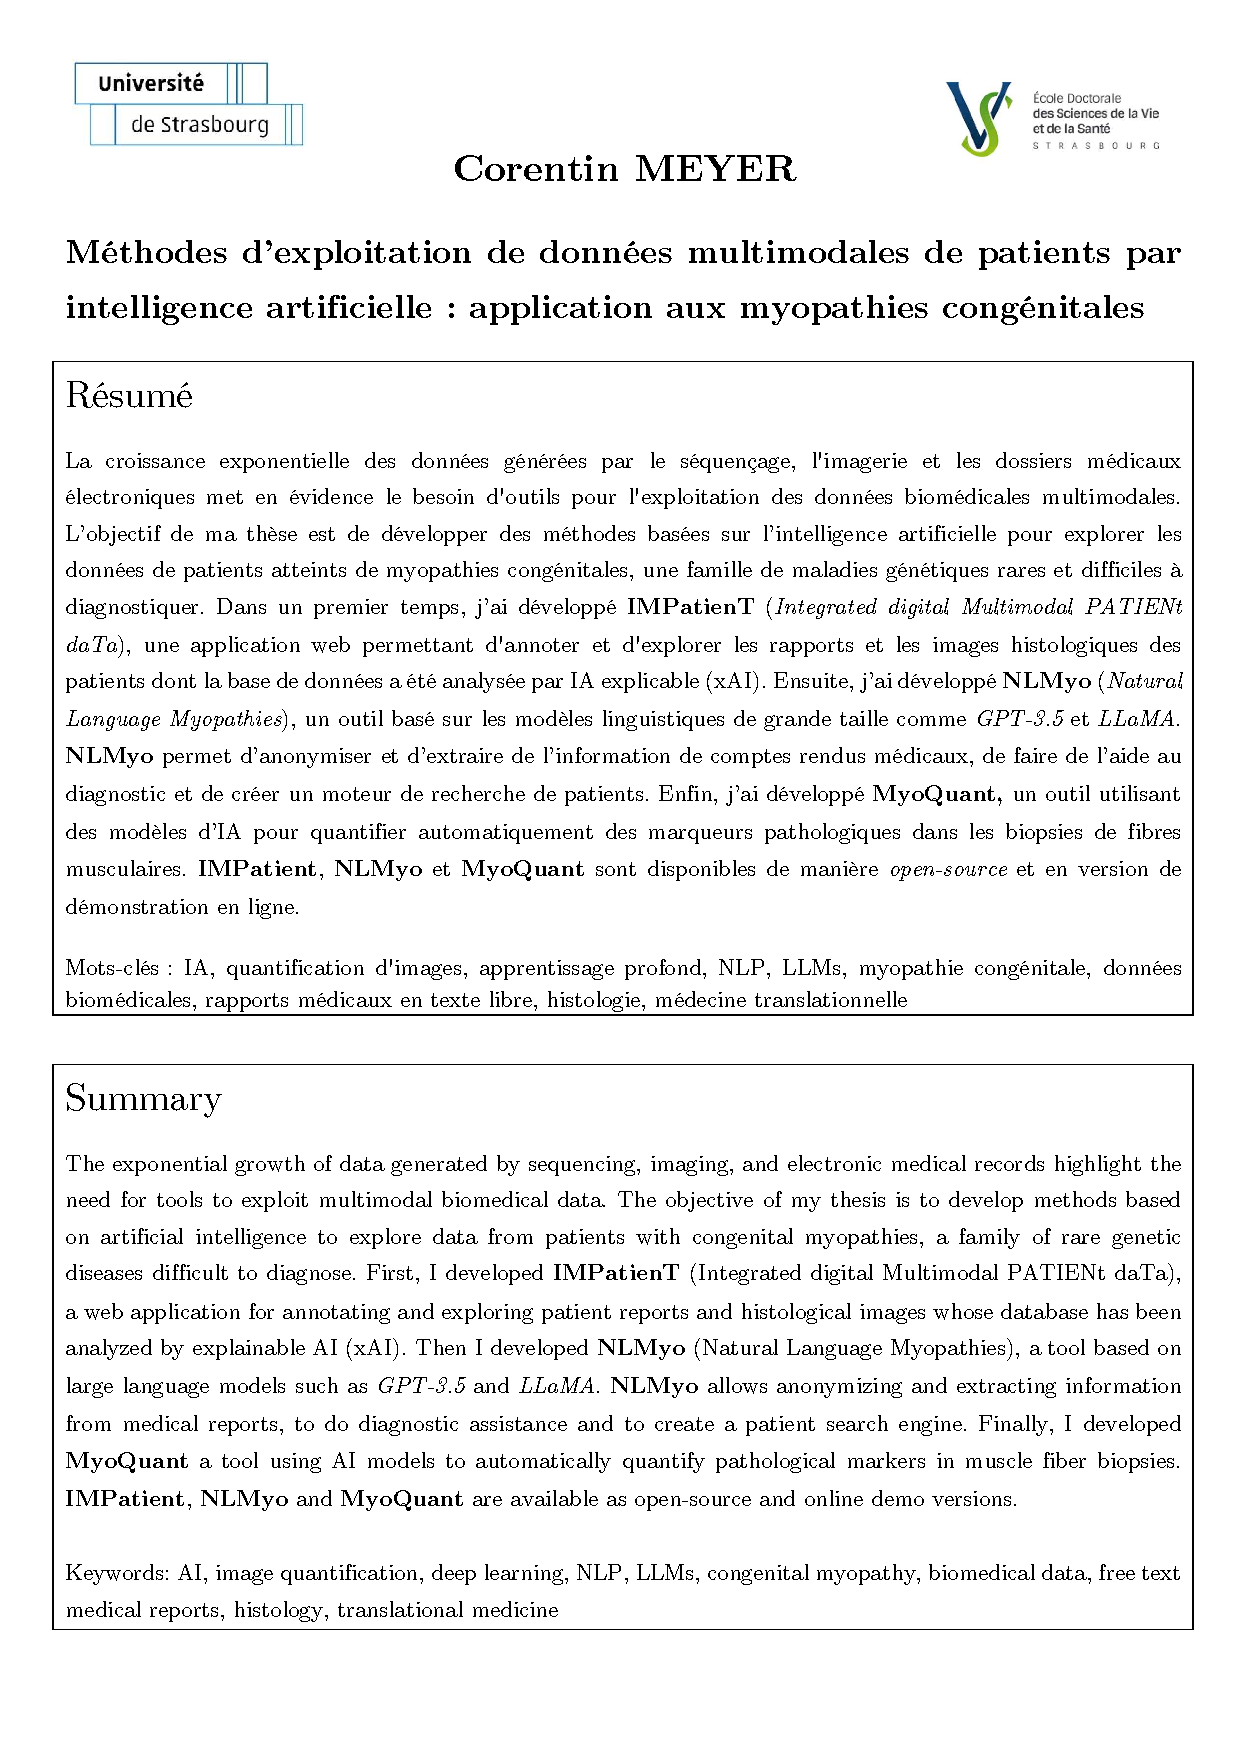
\includepdf[pages={1},scale=1,dpi=300]{corps/4emecouv.pdf}
%\makebackcover
\end{document}